% This is samplepaper.tex, a sample chapter demonstrating the
% LLNCS macro package for Springer Computer Science proceedings;
% Version 2.20 of 2017/10/04
%
\documentclass[runningheads]{llncs}
%
\usepackage{amsmath}
\usepackage{booktabs} % For pretty tables
\usepackage{caption} % For caption spacing
\usepackage{subcaption} % For sub-figures
\usepackage{graphicx}
\usepackage{rotating}
\usepackage{pgfplots}
\usepackage[all]{nowidow}
\usepackage[utf8]{inputenc}
\usepackage[margin=1in]{geometry}
\usepackage{tikz}
\usetikzlibrary{er,positioning,bayesnet}
\usepackage{multicol}
\usepackage{algpseudocode,algorithm,algorithmicx}
\usepackage{minted}
\usepackage{hyperref}
\usepackage{siunitx}
\usepackage{esdiff}
\usepackage{float}
\usepackage[inline]{enumitem} % Horizontal lists
% Used for displaying a sample figure. If possible, figure files should
% be included in EPS format.
%
% If you use the hyperref package, please uncomment the following line
% to display URLs in blue roman font according to Springer's eBook style:
% \renewcommand\UrlFont{\color{blue}\rmfamily}

\newcommand{\card}[1]{\left\vert{#1}\right\vert}
\newcommand*\Let[2]{\State #1 $\gets$ #2}
\definecolor{blue}{HTML}{1F77B4}
\definecolor{orange}{HTML}{FF7F0E}
\definecolor{green}{HTML}{2CA02C}

\pgfplotsset{compat=1.14}

\renewcommand{\topfraction}{0.85}
\renewcommand{\bottomfraction}{0.85}
\renewcommand{\textfraction}{0.15}
\renewcommand{\floatpagefraction}{0.8}
\renewcommand{\textfraction}{0.1}
\setlength{\floatsep}{3pt plus 1pt minus 1pt}
\setlength{\textfloatsep}{3pt plus 1pt minus 1pt}
\setlength{\intextsep}{3pt plus 1pt minus 1pt}
\setlength{\abovecaptionskip}{2pt plus 1pt minus 1pt}

\begin{document}

\title{AER303 Aerospace Laboratory - Aerodynamic Forces on an Airfoil}
%\titlerunning{Add subtitle}

\author{Eric Dai\inst{1} \and Jai Willems\inst{2} \and Mingde Yin\inst{3}}
%\authorrunning{F. Author et al.}

\institute{Division of Engineering Science, University of Toronto, Toronto, Canada \email{eric.dai@mail.utoronto.ca}\\ \and Division of Engineering Science, University of Toronto, Toronto, Canada \email{jai.willems@mail.utoronto.ca}\\ \and Division of Engineering Science, University of Toronto, Toronto, Canada\\ \email{mingde.yin@mail.utoronto.ca}}

\maketitle


% -----------------------------------------------------------------------------
%   Abstract
% -----------------------------------------------------------------------------


\begin{abstract}

In this report, the properties of the Clark Y airfoil are empirically explored at varying angles of attack by measuring airfoil surface and wake pressure distributions in a subsonic wind tunnel. The coefficient of pressure distributions, a momentum balance to determine the total drag, and numerical methods for the coefficients of lift, (pressure) drag, and moment are calculated. Empirical data measurements for these calculations are collected using two separate methods, and their comparative effectiveness is evaluated.\newline

Through analysis, it was found that the Clark Y airfoil appeared to stall at $\alpha\approx 13^\circ$. This conclusion was supported by the $C_P$ curves which showed a large plateau region for $\alpha\geq13^\circ$ indicating significant flow separation. For the same region, the $C_L$ curve experienced a significant drop in the lift slope and the $C_D$ curve had a sudden increase. No useful information could be extracted from the $C_M$ curve which remained relatively constant regarding the angle of attack.\newline

The empirically attained airfoil characteristics reflected the general trends and magnitudes of the values calculated from XFOIL and reported in the literature. This suggests that the results, within an experimental error, accurately reflect the true behaviour of a Clark Y airfoil in uniform flow at varying angles of attack.

\keywords{Airfoil \and Stall \and Inclined Manometer \and Scanivalve}
\end{abstract}


% -----------------------------------------------------------------------------
%   Nomenclature
% -----------------------------------------------------------------------------


\section{Nomenclature}

Refer to Table \ref{tab:nomenclature} for definitions and symbols common to this report.

\begin{table}[h]
    \centering
    \begin{tabular}{p{4.5cm}p{11cm}}
        \toprule
        Symbol/Term & Description \\
        \midrule
        $A'$ & Axial force per unit span. \\
        $C$ & Chord length. \\
        $C_D$ & Coefficient of Drag. \\
        $C_{D,p}$ & Coefficient of Drag based only on pressure drag. \\
        $C_L$ & Coefficient of lift. \\
        $C_M$ & Coefficient of Moment. \\
        $D'$ & Drag per unit span. \\
        $L'$ & Lift per unit span.\\
        $LE$ & Airfoil leading Edge. \\
        $M'$ & Moment of the airfoil around the leading edge per unit span. \\
        $N'$ & Normal force per unit span. \\
        $P_\ell$ & The pressure exerted on the airfoils lower surface. \\
        $P_u$ & The pressure exerted on the airfoils upper surface. \\
        $q_\infty$ & Free stream dynamic pressure. \\
        $Re$ & Reynolds number. \\
        $TE$ & Airfoil trailing edge. \\
        $U_\infty$ & Free stream velocity. \\
        Voltage-Pressure Measurement & A measurement of the pressure calculated at a point in the wind tunnel in the voltage space as returned by the data acquisition card. \\
        $\alpha$ & Angle of attack. \\
        $\Delta P$ & Dynamic pressure measurement. \\
        $\rho_\infty$ & Free stream density. \\
        $\theta$ & The angle made between the airfoils surface normal and the airfoils chord normal. \\
        \bottomrule
    \end{tabular}
    \caption{Commonly used symbols and terms.}
    \label{tab:nomenclature}
\end{table}


% -----------------------------------------------------------------------------
%   Introduction and Background
% -----------------------------------------------------------------------------


\section{Introduction and Background}\label{sec:introduction_and_background}

\noindent
This report aims to explore the experimental performance of a Clark Y airfoil at varying angles of attack, $\alpha$, to understand the characteristic dependency on the angle of attack. A secondary goal of the report is to evaluate the comparative effectiveness of two methods of measuring pressure distributions, and compare these methods to simulations and literature.\newline

\noindent
Airfoils are two-dimensional, wing cross-sections that produce lift by accelerating flow over their contour which result in a surface pressure distribution that can cause a net lifting action. At the same time, airfoils produce drag forces through skin friction and fluid viscosity. The combination of both the lift and drag forces impart a pitching moment on the airfoil which, in aircraft design, must be balanced by the horizontal stabilizer. Since the lift, drag, and moment forces depend on the airfoil's pressure distribution which varies with the angle of attack, the performance of the airfoil in producing sufficient lift to sustain flight will thusly depend on the angle the airfoil makes with the relative airflow. Gaining insight into the angle of attack evolution of the airfoil's lift, drag, and moment is necessary for learning the stall and performance characteristics of the airfoil which are necessary in aircraft design.\newline

\subsection{Normal, Axial, and Moment Forces}

\noindent
Ignoring viscous effects, the normal and axial forces on an airfoil describe the net effect of a pressure distribution over the airfoil. The normal force is the net pressure force exerted normal to the aircraft's chord. In contrast, the axial force is the net pressure force acting parallel to the aircraft's chord. These forces yield lift and pressure drag forces when combined with the angle of attack as will be discussed in section \ref{sec:LDC}.\newline

\noindent
With an airfoil in a uniform flow, let $P_u$ and $P_\ell$ be the pressure distributions over the airfoil's top and bottom surfaces respectively. Additionally, let $\theta$ be the angle between the chord normal and the airfoil surface normal measured clockwise. From these measures, the normal and axial forces acting on the airfoil can be calculated using equations \ref{eq:normal_force} and \ref{eq:axial_force} where the normal and axial components are summed over the airfoil's surface to yield the net normal and net axial component. The normal and axial definitions can be represented pictorially in figure \ref{fig:airfoil_directions} where the expressed forces define their positive orientations. In a similar approach, the moment around the leading edge of the airfoil is given by equation \ref{eq:leading_edge_moment} which integrates the product of the moment arm and force acting in both the normal and axial direction. A positive moment value is defined to be the angular direction that increases the angle of attack.\newline

\begin{align}
    N' &= \int_{LE}^{TE} -P_u\cos\theta ds_u + \int_{LE}^{TE} P_\ell\cos\theta ds_\ell
    \label{eq:normal_force}\\
    A' &= \int_{LE}^{TE} -P_u\sin\theta ds_u + \int_{LE}^{TE} P_\ell\sin\theta ds_\ell
    \label{eq:axial_force}\\
    M' &= \int_{LE}^{TE} \left[(P_u\cos\theta)x - (P_u\sin\theta)y\right]ds_u + \int_{LE}^{TE} \left[(-P_\ell\cos\theta)x + (P_\ell\sin\theta)y\right]ds_\ell
    \label{eq:leading_edge_moment}
\end{align}

\subsection{Calculating Lift, Drag and Dimensionless Coefficients}\label{sec:LDC}

\noindent
The lift of an airfoil is defined as the net force exerted on the airfoil normal to the relative airflow, whereas the drag is the net force parallel to the relative airflow. These forces per unit span can be calculated using equations \ref{eq:lift} and \ref{eq:drag} where the angle of attack, $\alpha$, is the angle between the airfoil's chord line and the relative airflow. The lift and drag definitions can be represented pictorially in figure \ref{fig:airfoil_directions} where the expressed forces define their positive orientations.\newline

\begin{align}
    L' &= N'\cos\alpha - A'\sin\alpha \label{eq:lift} \\
    D' &= N'\sin\alpha + A'\cos\alpha \label{eq:drag}
\end{align}

%% TEST: Does a diagram like this look good?
\begin{figure}
    \centering
    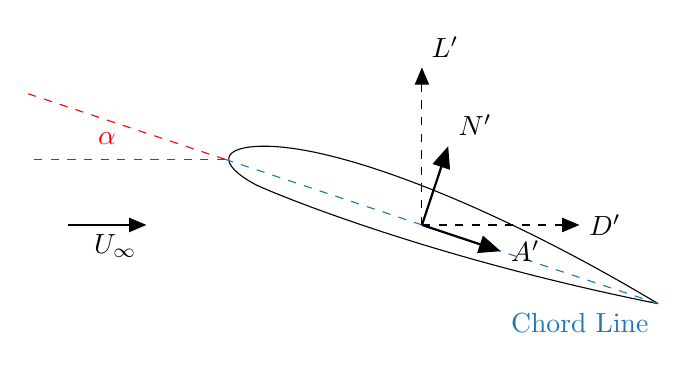
\begin{tikzpicture}
        \draw[rounded corners = 1cm] (6,-2)  .. controls (4, -0.8) and (2,0)  .. (0, 0) .. controls (1, -0.55) and (3, -1.4) .. (6,-2);
        \draw[dashed, blue] (0.5,-0.1666) -- (6,-2) node[anchor=north east] {Chord Line};
        \draw[dashed, red] (0.5,-0.1666) -- (-2,0.666);
        \draw[dashed, red] (0.5,-0.1666) -- (-2, -0.1666);
        \draw[red] (-1, 0.1) node {$\alpha$};
        \draw[->] (-1.5,-1) -- (-0.5,-1) node[anchor=north east] {$U_\infty$};
        \draw[thick,->] (3, -1) -- (3.3333, 0) node[anchor=south west] {$N'$};
        \draw[thick,->] (3, -1) -- (4, -1.333) node[anchor=west] {$A'$};
        \draw[dashed, ->] (3, -1) -- (3, 1) node[anchor=south west] {$L'$};
        \draw[dashed, ->] (3, -1) -- (5, -1) node[anchor=west] {$D'$};
    \end{tikzpicture}
    \caption{Definition of variables related to forces on an airfoil}
    \label{fig:airfoil_directions}
\end{figure}

\noindent
To express the performance of an airfoil in a manner that is quasi-decoupled from the flow properties, the lift, drag, moment, and pressure distributions are often expressed in nondimensionalized form.

\noindent
The nondimensionalized pressure can be found using using equation \ref{eq:cp} where $q_\infty\equiv\frac{1}{2}\rho_\infty U_\infty^2$ is the freestream dynamic pressure. and $\Delta P$ is the difference between the local and freestream static pressures.\newline

\begin{equation}
    C_p = \frac{\Delta P}{q_\infty}
    \label{eq:cp}
\end{equation}

\noindent
Lift, drag, and moment can also be nondimensionalized using equations \ref{eq:cl}, \ref{eq:cd}, and \ref{eq:cm} respectively, where $C$ is the airfoil's chord length.\newline

\begin{multicols}{3}
\begin{equation}
    C_L = \frac{L'}{q_\infty C}
    \label{eq:cl}
\end{equation}
\begin{equation}
    C_D = \frac{D'}{q_\infty C}
    \label{eq:cd}
\end{equation}
\begin{equation}
    C_M = \frac{M'}{q_\infty C^2}
    \label{eq:cm}
\end{equation}
\end{multicols}

\subsection{Calculating Total Drag from Wake Velocity}

\noindent
The drag force formulation stated earlier (equation \ref{eq:drag}) ignores viscous effects because this experiment cannot directly measure the shear force distribution over the surface of the airfoil. That means the force in equation \ref{eq:drag} only gives pressure drag. The total drag, typically a value of interest is calculated by performing a momentum balance in a control volume containing the airfoil, to determine how much the airfoil has decelerated the flow around it. The equation to calculate the total drag per unit span is given in equation \ref{eq:wake_drag}.\newline

\begin{align}
    D' &= \rho\int_{\text{rake}} u (U_\infty - u) dy \label{eq:wake_drag}
\end{align}

\subsection{Stall}

\noindent
An airfoil stall is characterized by a significant separation of flow from the airfoil surface resulting in several effects that can be observed in the dimensionless curves.

\begin{itemize}

    \item When flow separation occurs, the $C_P$ distribution plateaus in the region of separation as separation will occur in the presence of non-favourable pressure gradients.
    
    \item As $\alpha$ increases, $C_L$ increases linearly until it reaches a peak and then falls sharply. The peak and fall of the $C_L$ curve is a result of flow separation causing the pressure distribution to plateau, reducing the pressure difference needed to generate lift.
    
    \item The flow separation associated with an impending stall incurs higher drag from viscous effects, resulting in a dramatically increasing $C_D$ for all angles of attack above the minimum stall angle (critical angle of attack).
    
    \item $C_{M, LE}$ remains a nearly constant negative value. Even when the airfoil stalls, the pitching moment at the leading edge is not affected as the pressure gradient happens most drastically at the leading edge, which does not affect the moment at the leading edge.
    
\end{itemize}

\noindent
Stalled conditions lead to unpredictable behaviour of an airfoil and reduced aircraft controllability as the lack of airflow over control surfaces cause a slow and sloppy control response. It is important to understand the behaviour of varying the angle of attack on the lift, drag, and moment characteristics of an airfoil to understand its limitations.


% -----------------------------------------------------------------------------
%   Experimental Set-Up
% -----------------------------------------------------------------------------


\section{Experimental Set-Up}

\noindent
This section details the lab setup and procedure used in the experiment.

\subsection{Apparatus}

\noindent
The Clark Y airfoil specimen used in the experiment is a 3D printed model, with 19 holes along the centerline of the span allowing pressure measurements over the surface. The pressure tap locations are presented in table \ref{tab:pressure_taps}.\newline

\begin{table}
    \centering
    \begin{tabular}{|c||c|c|c|c|c|c|c|c|c|c|}\hline
        x/c & 0 & 0.03 & 0.06 & 0.10 & 0.15 & 0.20 & 0.30 & 0.40 & 0.55 & 0.70 \\\hline
        Tap Number & 1 & 2 & 3 & 4 & 5 & 6 & 7 & 8 & 9 & 10\\\hline \hline
        x/c & 0.85 & 1.00 & 0.90 & 0.60 & 0.40 & 0.30 & 0.20 & 0.10 & 0.05&\\\hline
        Tap Number & 11 & 12 & 13 & 14 & 15 & 16 & 17 & 18 & 19&\\\hline
    \end{tabular}
    \caption{Static pressure tap locations for the test model. Taps 1 through 12 are located on the top surface, while 13 thought 19 are located on the bottom surface.}
    \label{tab:pressure_taps}
\end{table}

\noindent
The tests on the airfoil are conducted in an ELD Model 402B subsonic open-return wind tunnel, with a 304.8 x 304.8 x 610 mm  square prismatic test section. The airfoil is shown installed in the wind tunnel in figure \ref{fig:wind_tunnel_setup}. The airfoil is secured using a rotary mechanism to vary the angle of attack across trials and can be seen in figure \ref{fig:aoa_select}.\newline

\begin{figure}
    \centering
    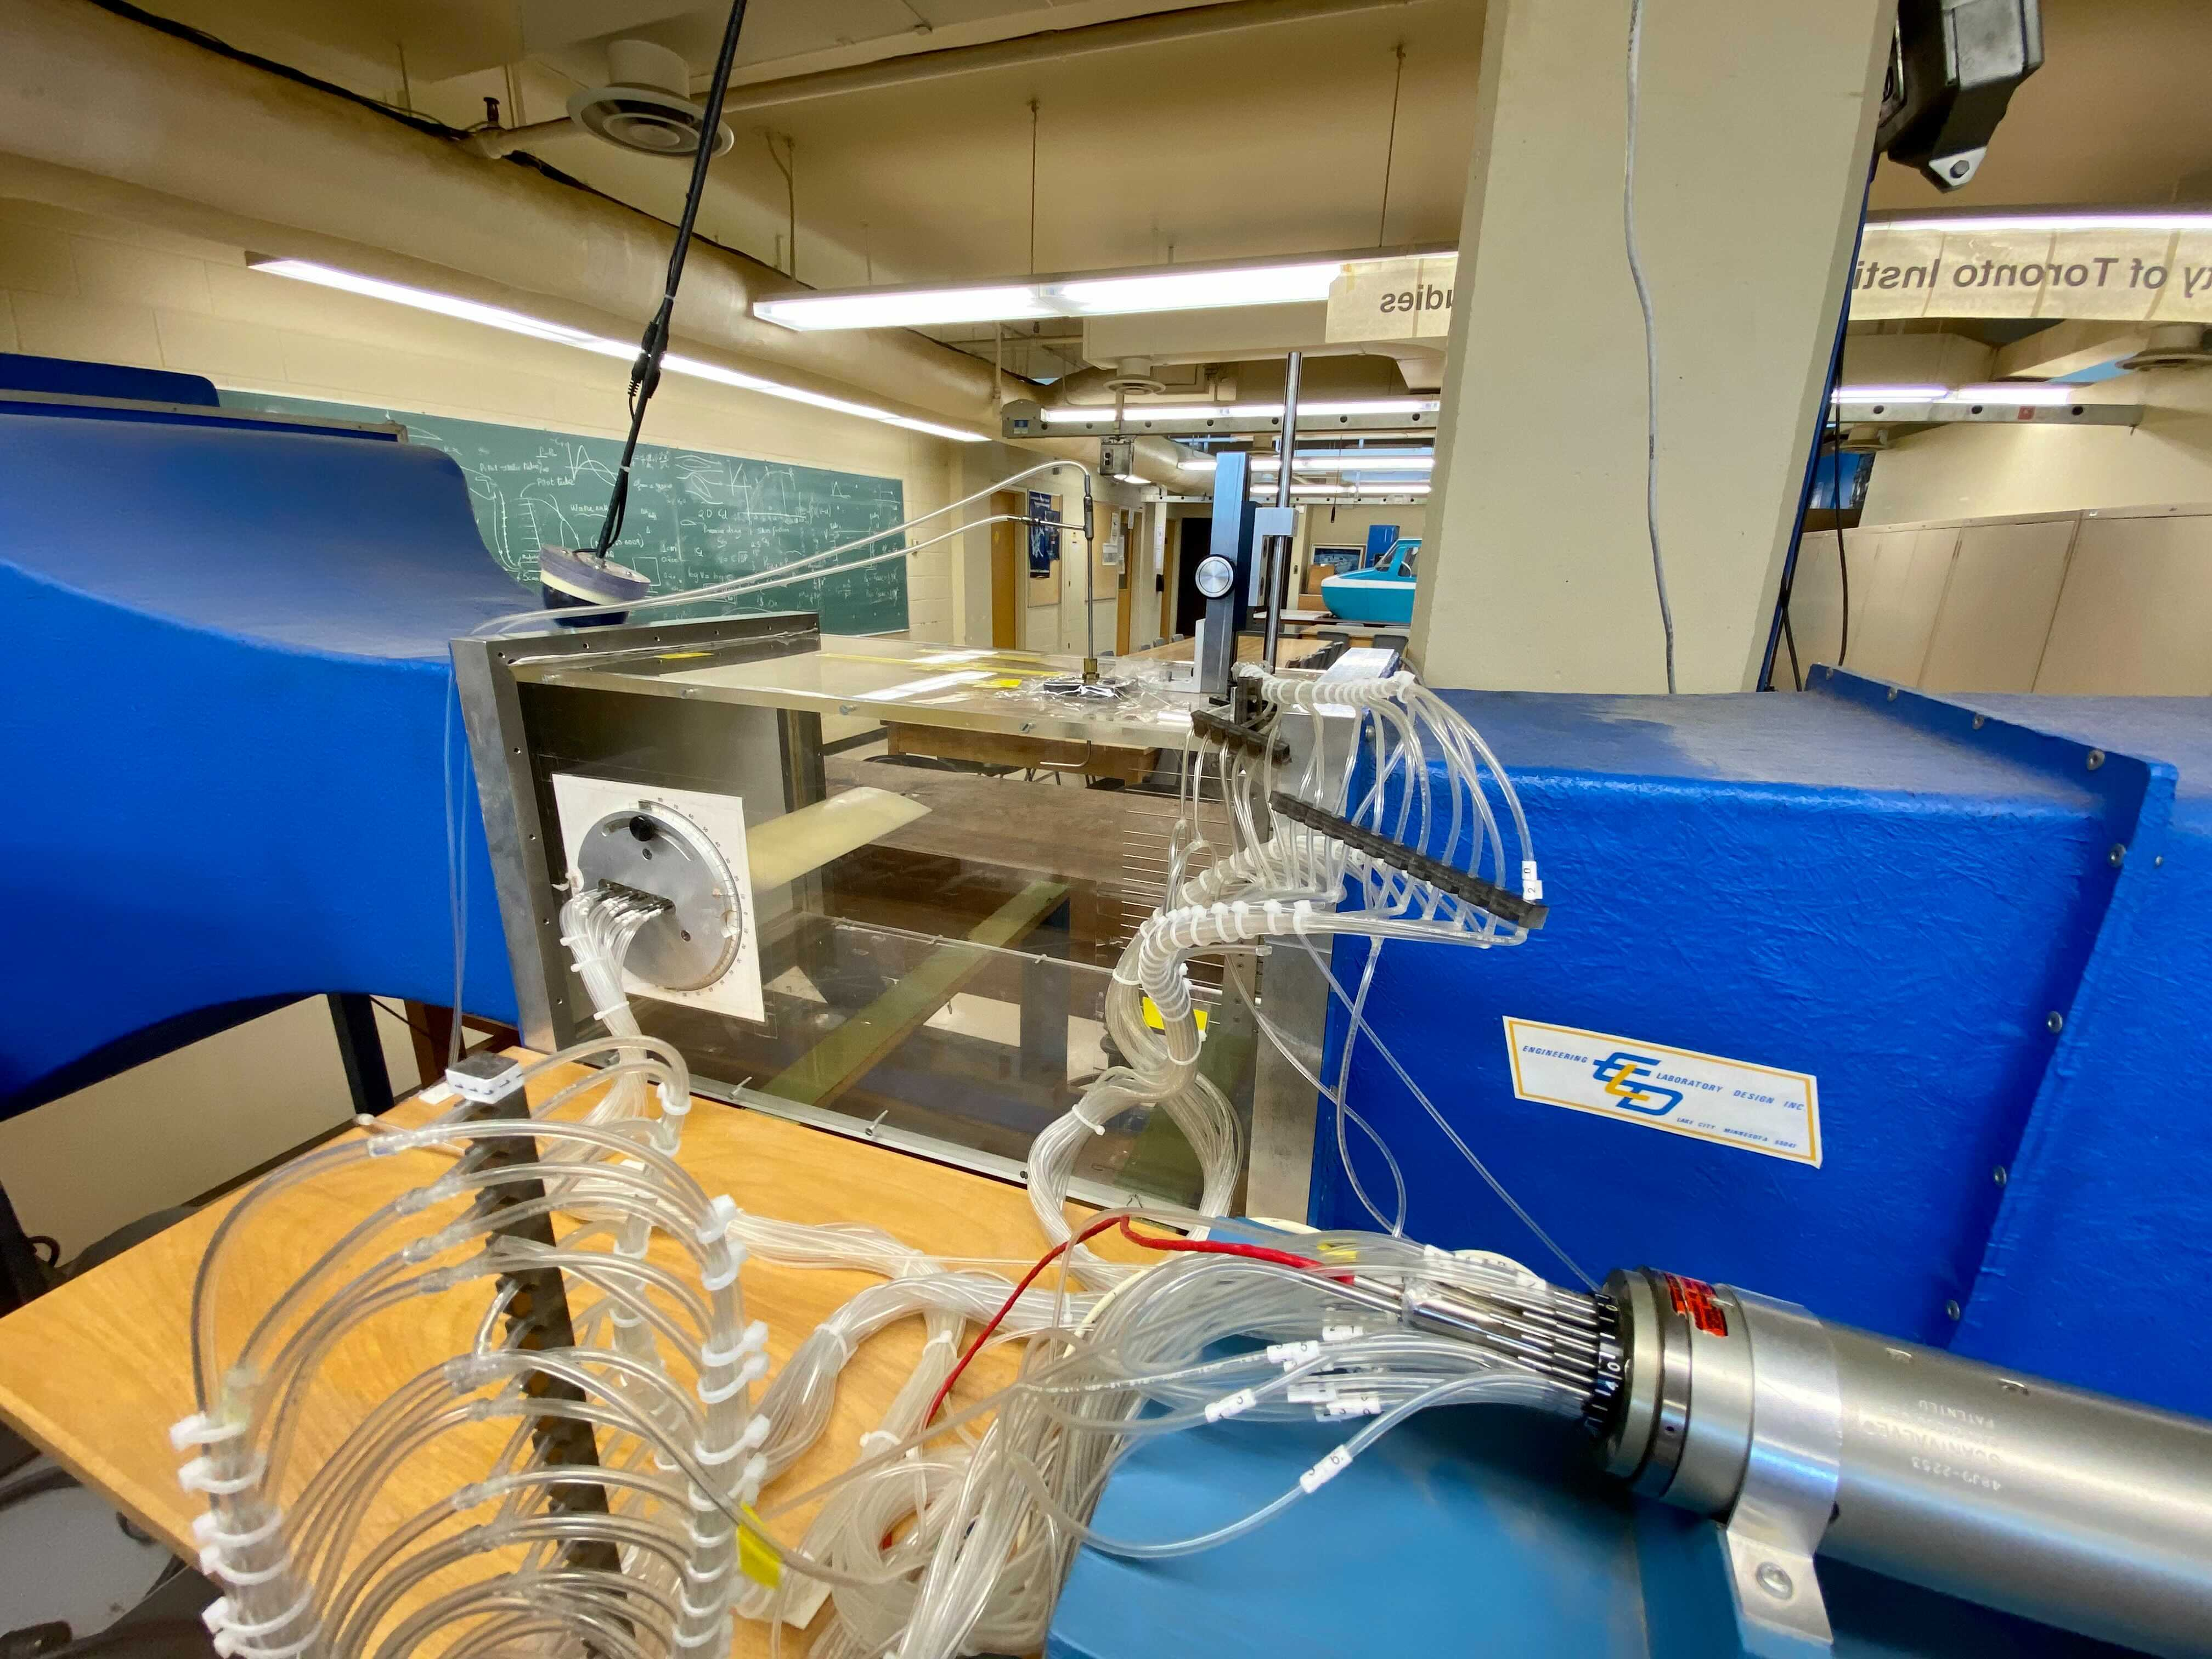
\includegraphics[width=0.6\textwidth]{Apparatus Pictures/wind_tunnel_setup.jpg}
    \caption{The wind tunnel section, with the 3D printed test model installed.}
    \label{fig:wind_tunnel_setup}
\end{figure}

\begin{figure}
    \centering
    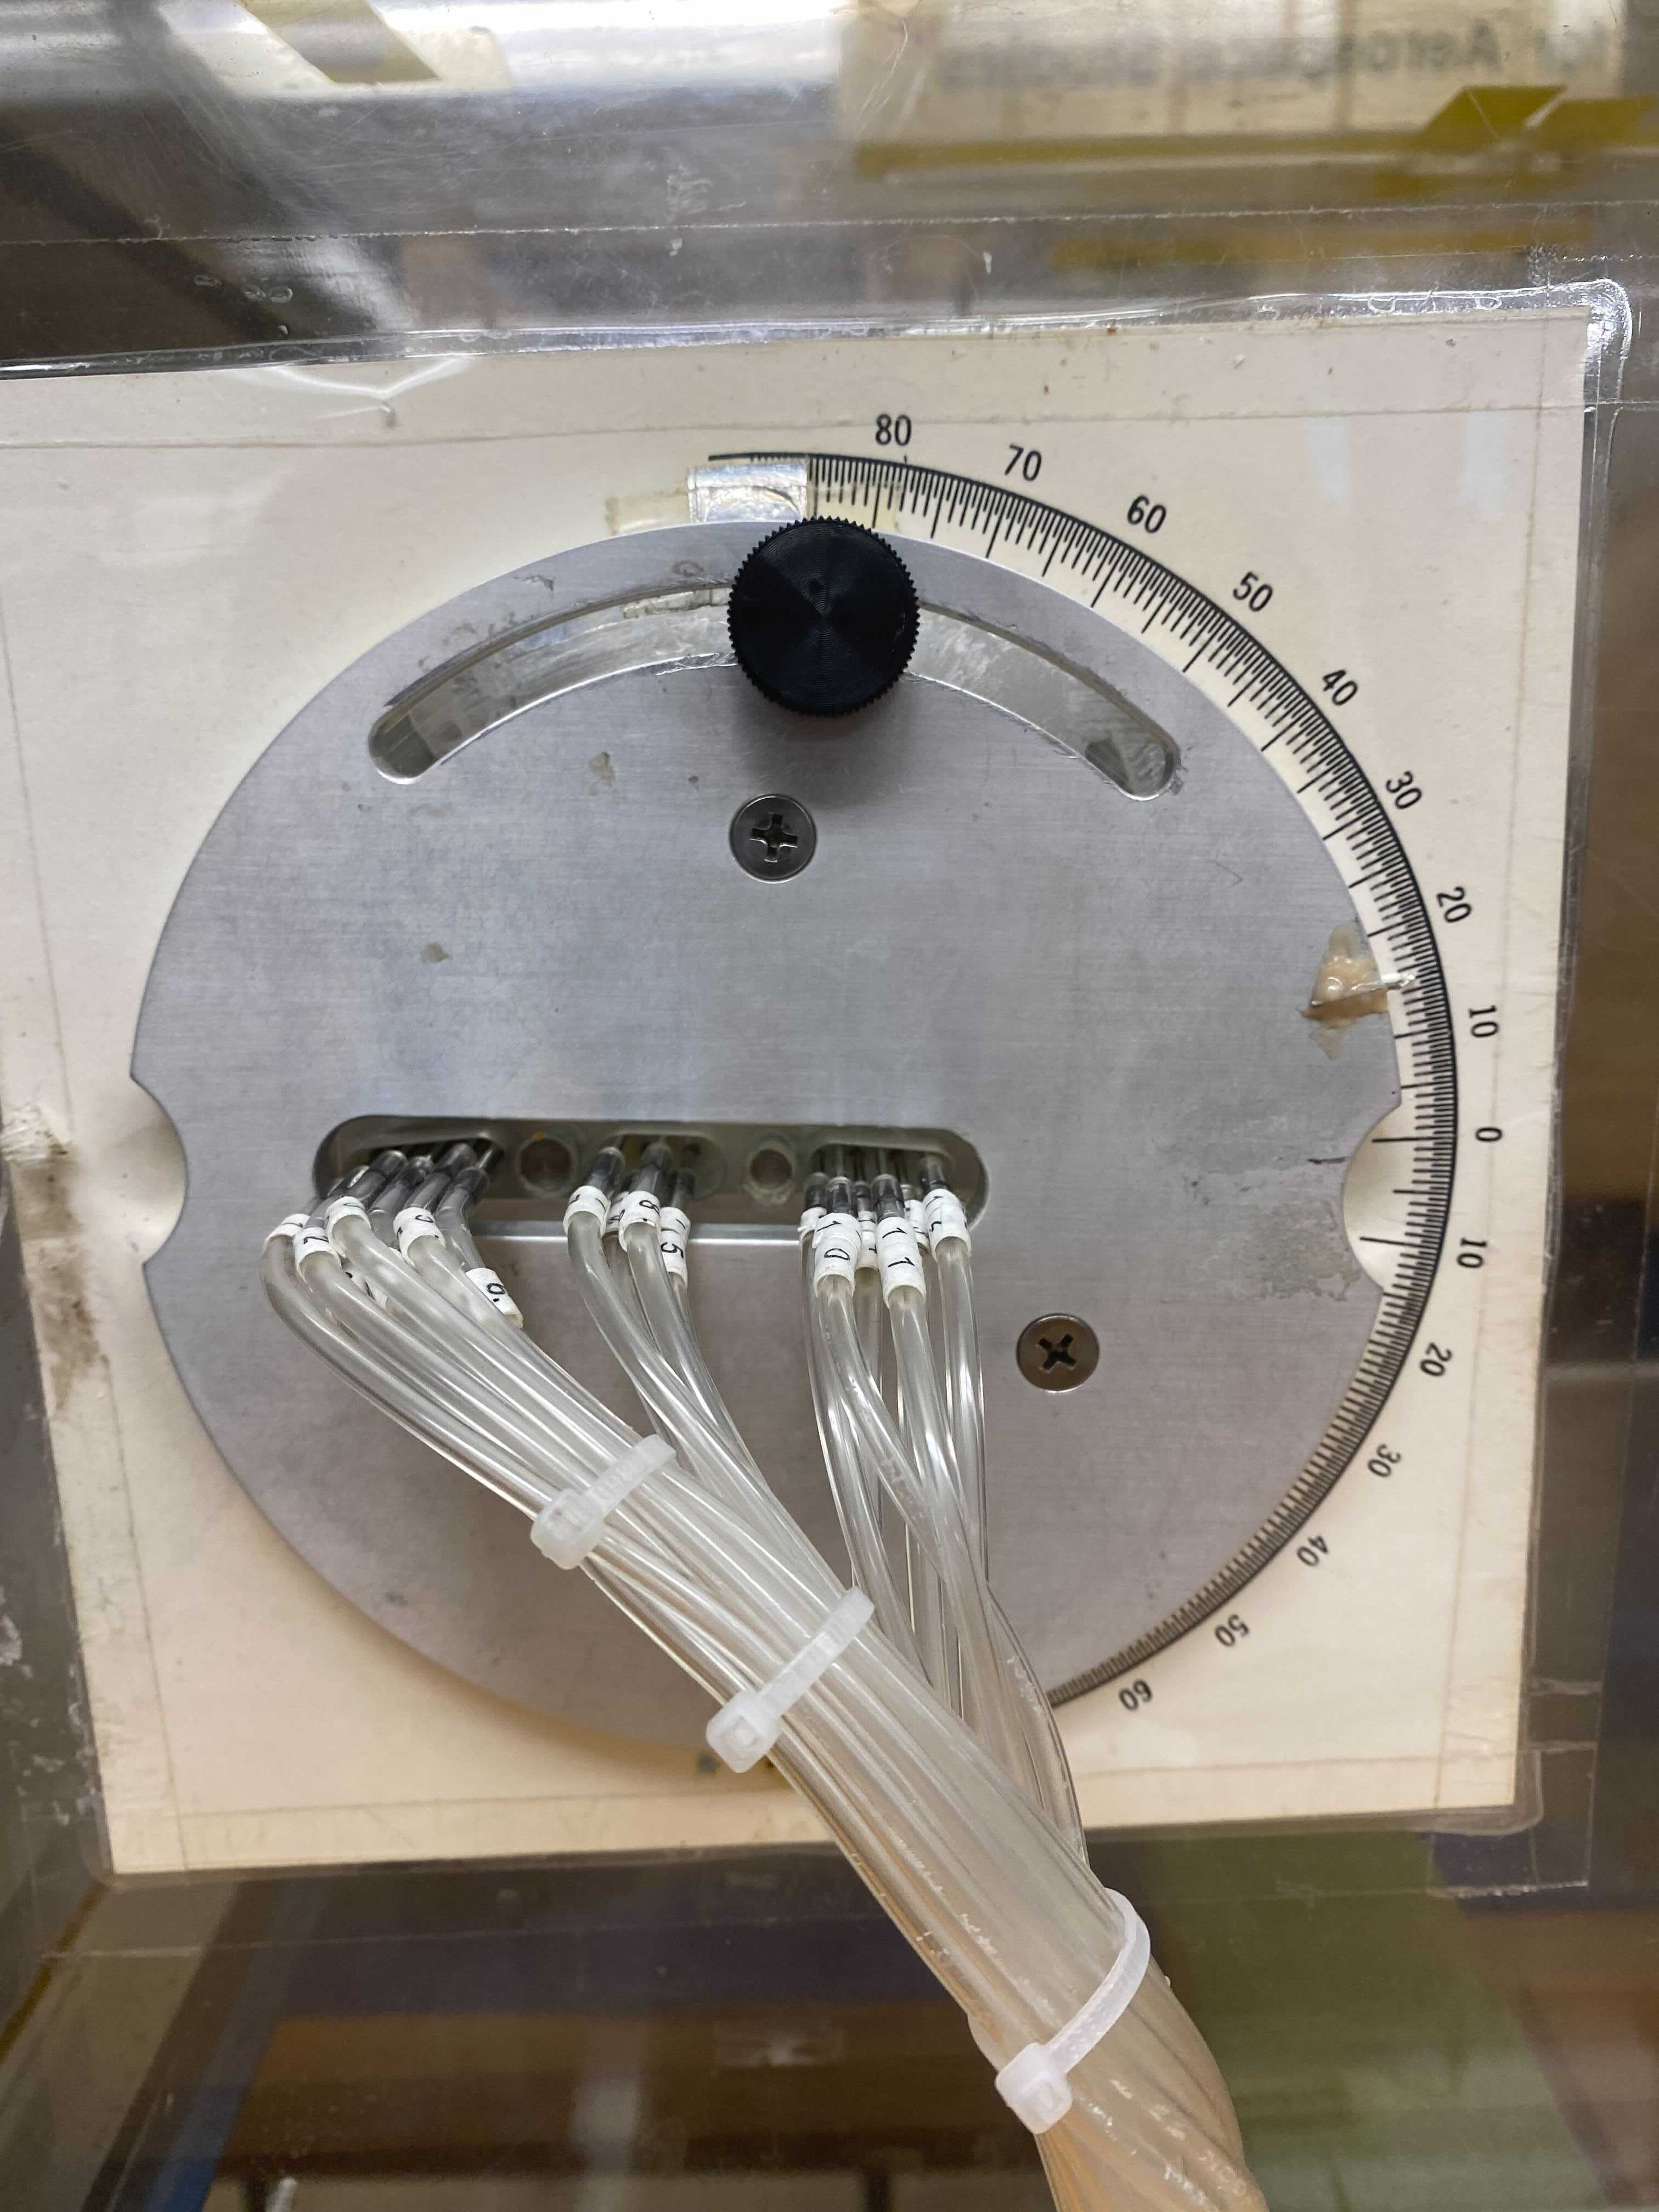
\includegraphics[width=0.4\textwidth]{Apparatus Pictures/aoa_selector.jpg}
    \caption{Adjustable rotary mechanism to hold the airfoil at different angles of attack.}
    \label{fig:aoa_select}
\end{figure}

\noindent
In addition to the 19 static pressure taps on the airfoil, there are 17 pitot tubes arranged as a rake, placed $27\si{cm}$ downstream of the airfoil's trailing edge. A pitot-static tube placed upstream of the airfoil is used for wind tunnel speed measurements, with the pitot tube connected to a Betz manometer and the static tube used as the reference pressure in the two measurement devices.\newline

\noindent
A total of 38 pressure tubes exit the wind tunnel; one is the upstream pitot tube connecting to the Betz manometer while the other 37 connect to the measurement devices. The latter 37 tubes are bifurcated to feed into both a multi-channel Scanivalve-transducer system and an inclined manometer.\newline

\noindent
The Scanivalve system is pictured in figure \ref{fig:scanivalve} and is responsible for redirecting a specific pressure tube to an output measuring device. The analog pressure transducer is connected to the sampling and reference outputs of the Scanivalve. The connected Scanivalve rapidly switches between the 36 pressure tubes such that the pressure transducer measures the pressure difference between the sampled pressure and the reference pressure from the upstream static tube. The analog signal from the pressure transducer is fed into a data acquisition card connected to a computer running MATLAB to collect the data.\newline

\begin{figure}[h]
    \centering
    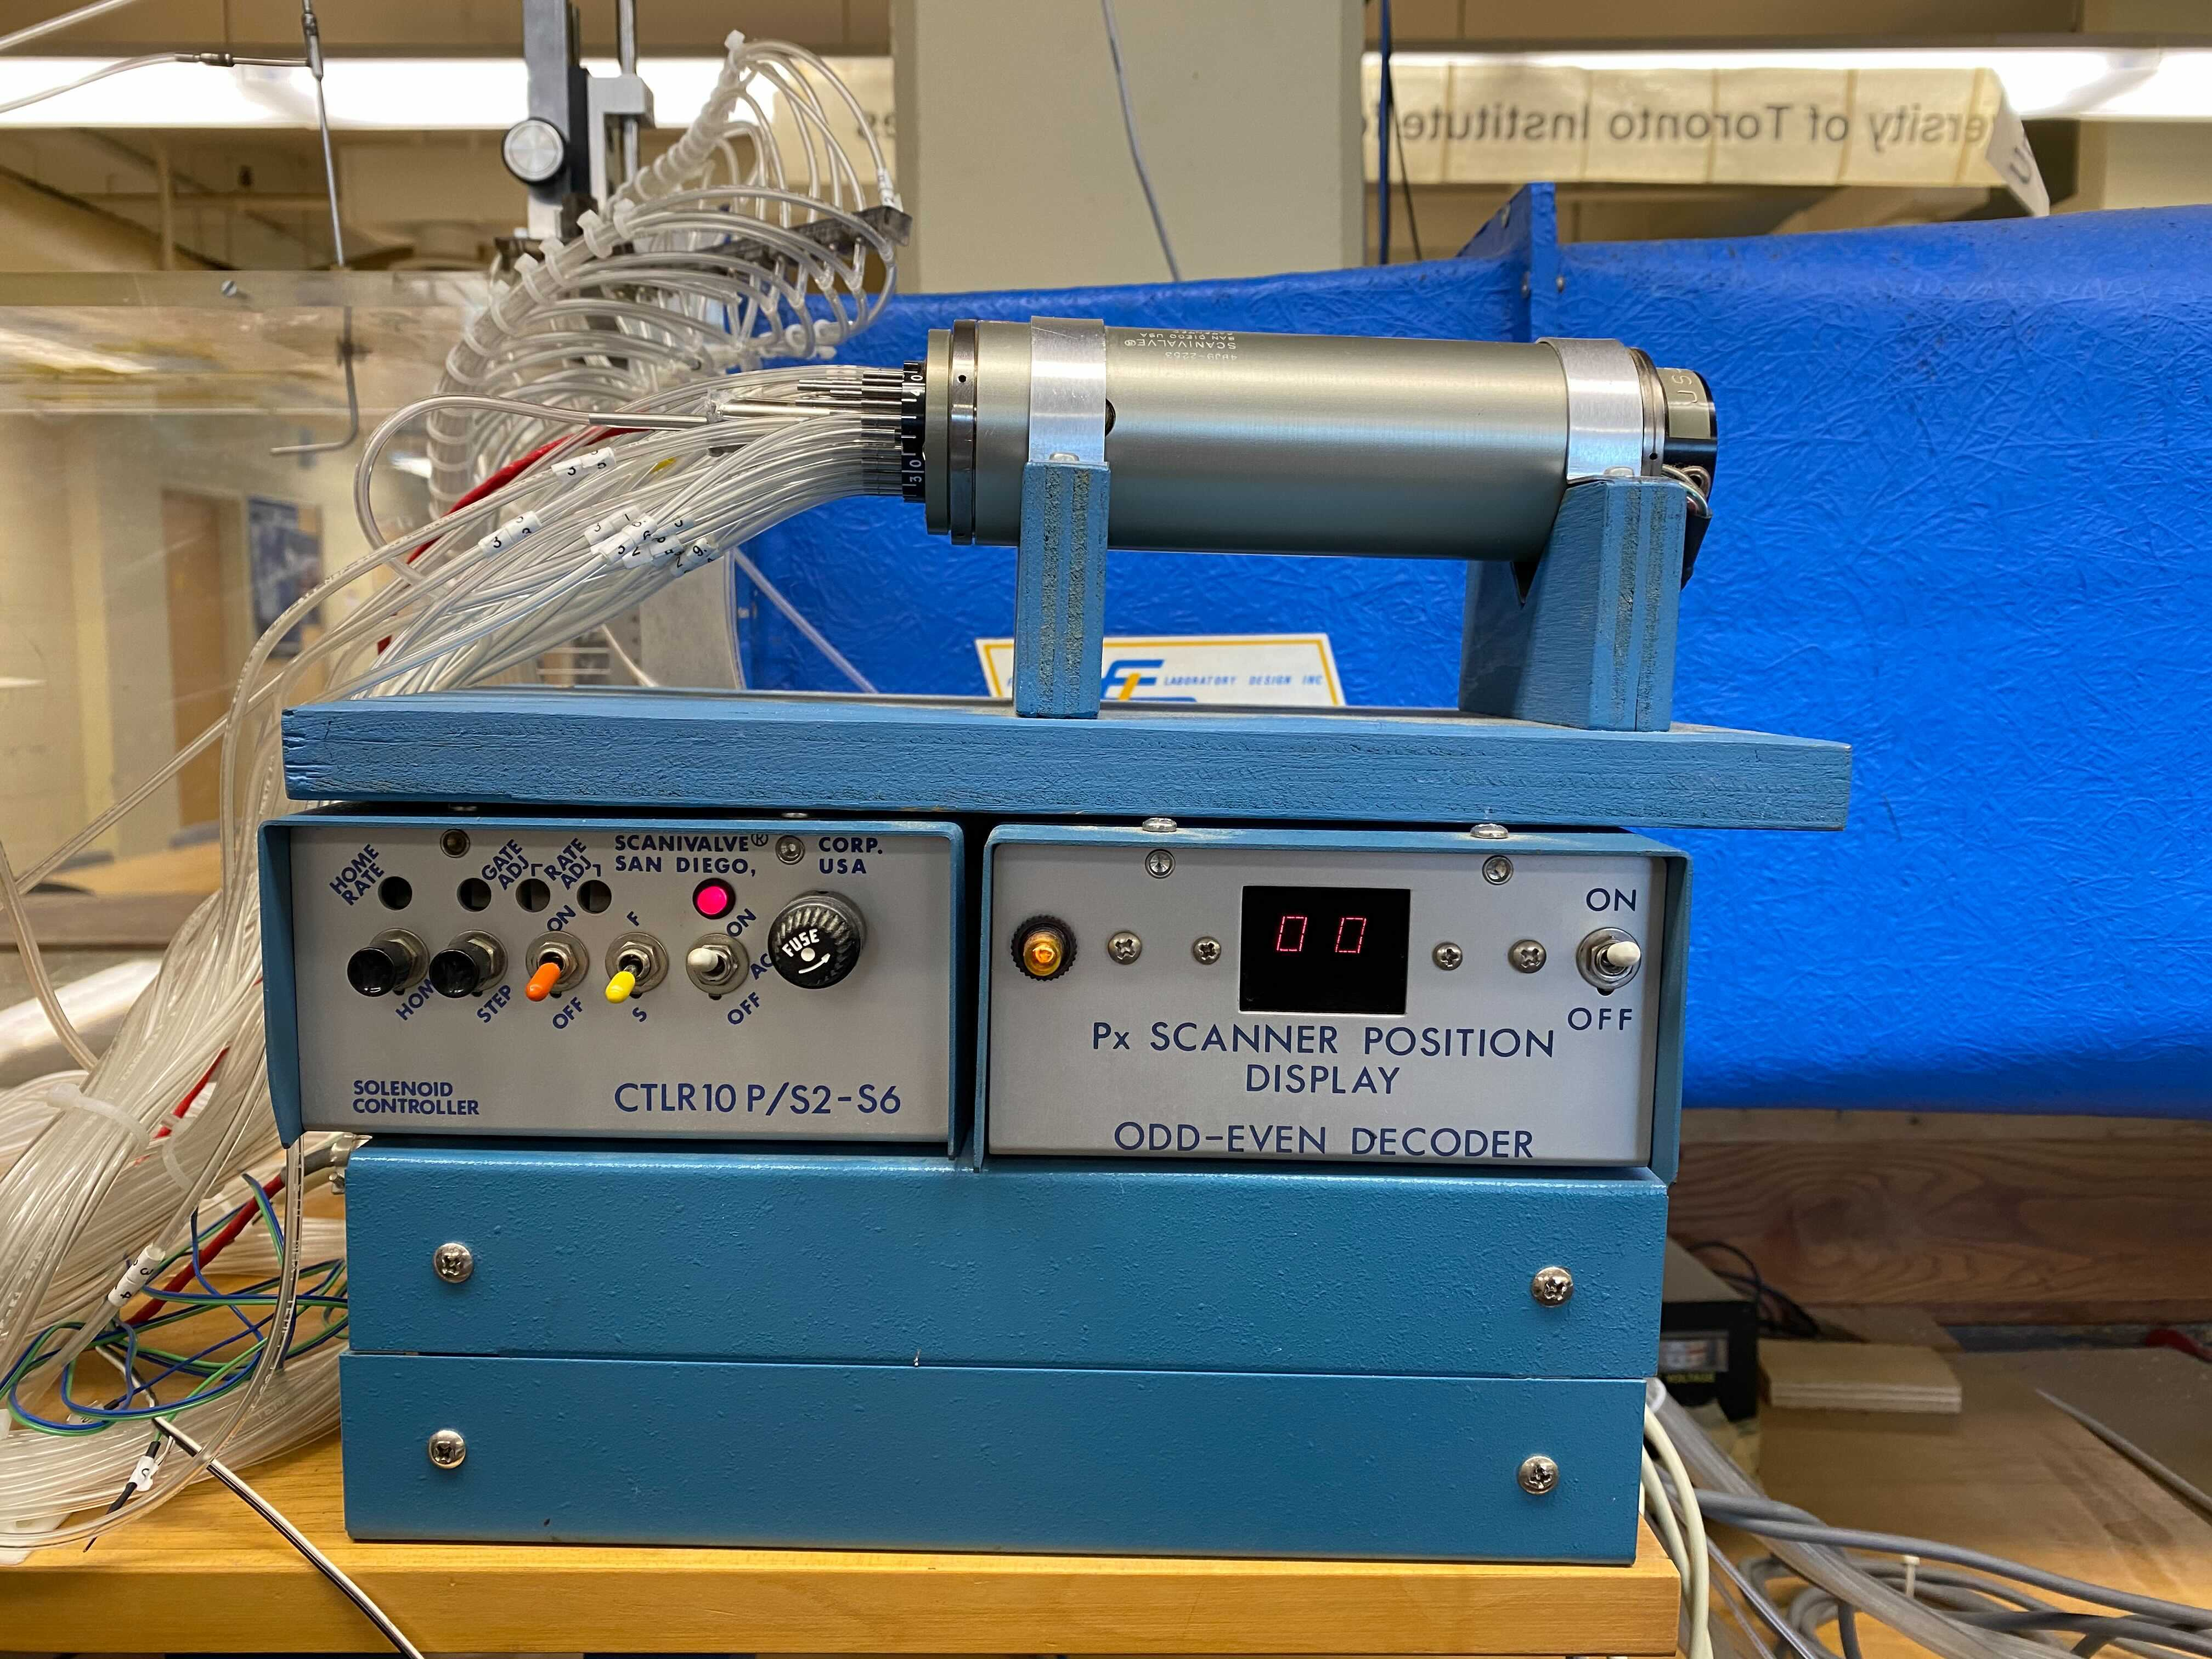
\includegraphics[width=0.4\textwidth]{Apparatus Pictures/scanivalve.jpg}
    \caption{Scanivalve system, connected to a pressure transducer. The system allows for rapid switching between the 36 channels to allow the transducer to sweep through all pressure inputs.}
    \label{fig:scanivalve}
\end{figure}

\noindent
The inclined manometer takes in 36 input channels and one reference channel to measure the pressure difference between each of the 36 inputs compared to the reference pressure which is set to that of the upstream static tube.

\begin{figure}[h]
    \centering
    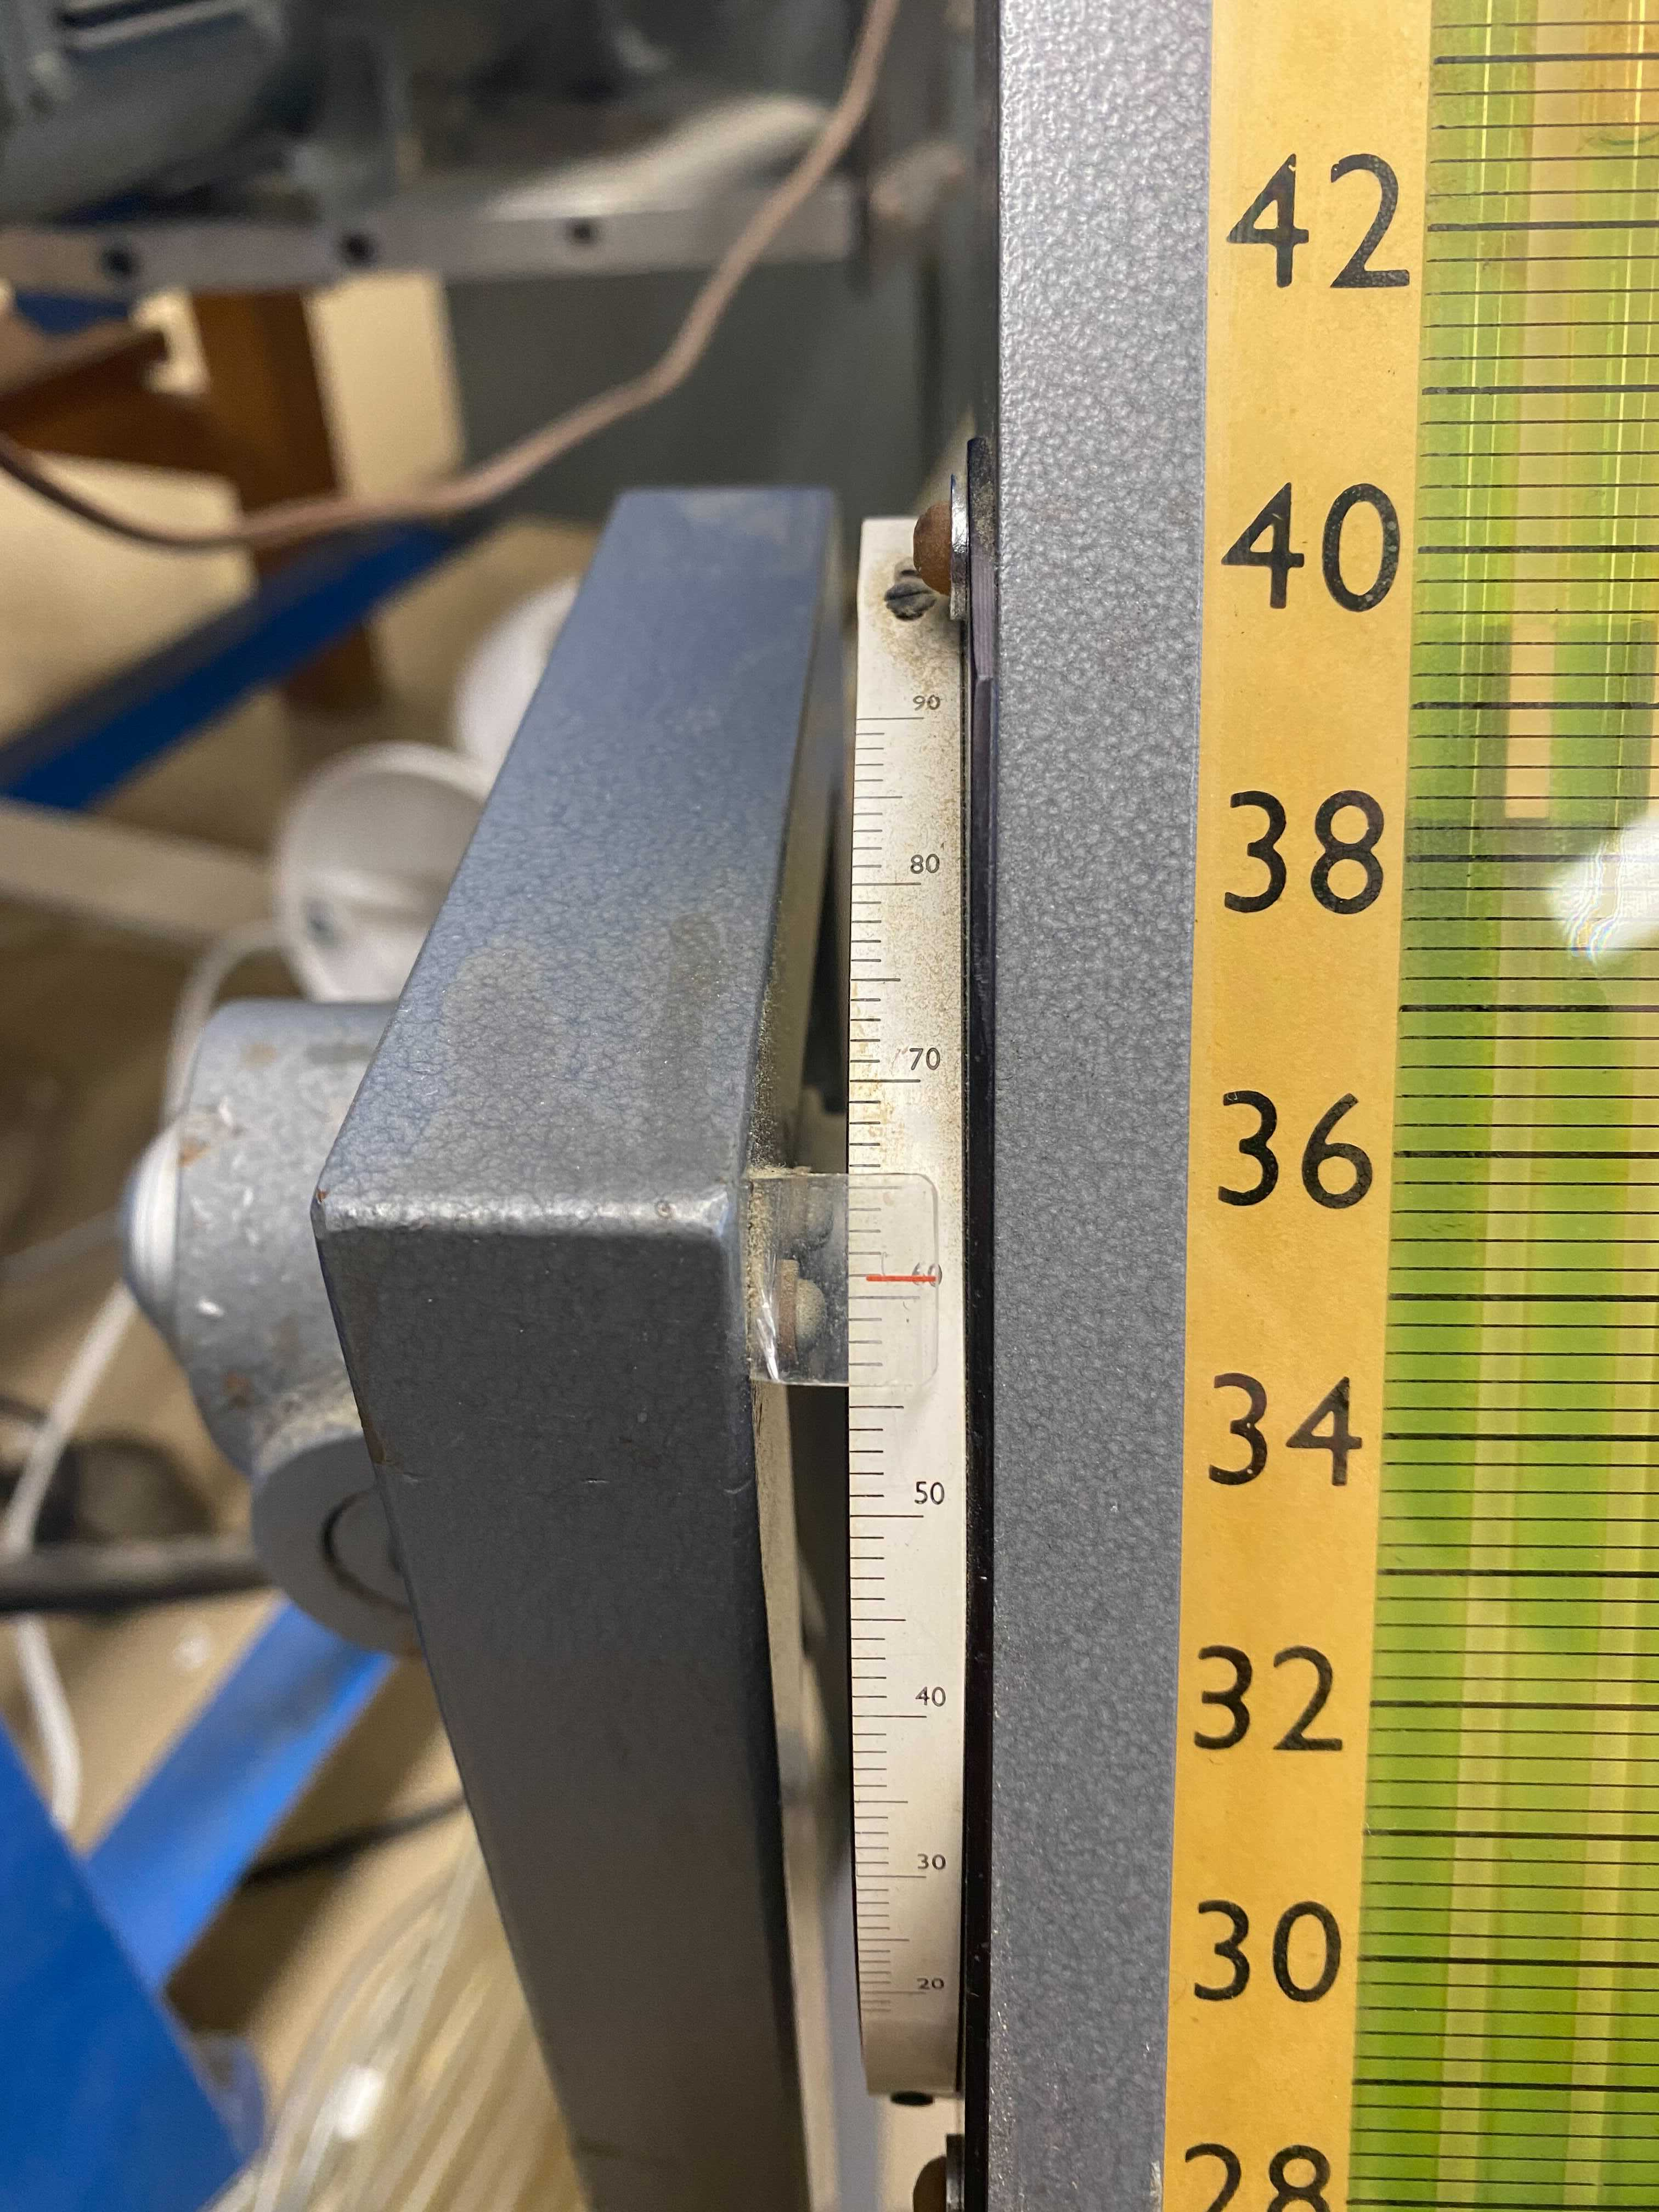
\includegraphics[width=0.4\textwidth]{Apparatus Pictures/inclined_manometer_slope_graduations.jpg}
    \caption{Inclined manometer slope graduations.}
    \label{fig:manometer}
\end{figure}

\subsection{Procedure}\label{sec:procedure}

% What is measured and how it is acquired.

\noindent
The procedure used for acquisition of pressure measurements is as follows:

\begin{enumerate}

    \item The sample frequency and data acquisition time are determined such that the pressure transducer measurements admit a $\pm 1\%$ accuracy. The wind tunnel speed is set to $110\si{km.h^{-1}}$. A series of representative measurements from the pressure transducer output are then taken and autocorrelated to determine the sample frequency and data acquisition time required for $\pm 1\%$ accuracy.
    
    \item The calibration curve for the pressure transducer is constructed next. This allows interpolated conversion from voltage-pressure representations of pressure transducer measurements into equivalent pressure values. The curve is constructed by taking ten different voltage-pressure measurements at varying wind tunnel speeds using scanivalve readings while finding the corresponding pressure measurements using the Betz manometer. This correspondence between representations is used to calibrate the pressure-voltage curve of the transducer.
    
    \item The wind tunnel speed is set back to $110\si{km.h^{-1}}$ and wind tunnel's pitot-static pressure difference is measured to calculate the actual wind speed experienced in the wind tunnel.
    
    \item Next, the angle of attack is changed in the positive and negative directions to determine the angle of attack associated with the airfoil stall. Using this information, it is determined what angles of attack would be useful to measure to accurately represent the airfoil properties up to and past stall conditions. The angle of attack values chosen were \numlist{0;3;6;8;10;11;13;15;16;17;20} degrees.

    \item Cycling through each angle of attack, the pressure distribution is measured along the top and bottom surfaces of the airfoil in addition to the pressure distribution in the airfoils wake. These values are measured by reading the fluid height changes from the inclined manometer. To get greater precision in the wake measurements, the wake rake is displaced by $5\si{mm}$ for a second round of measurements to fill the gaps between each rake tube. Pressure measurements are taken using two methods: (1) the pressure transducer fed by the scanivalve device and (2) the inclined manometer.

\end{enumerate}

\noindent
Due to equipment malfunction with the Betz manometer, steps 1 and 2 are not performed, and instead a pre-made calibration curve for the pressure transducer is provided ($P = 115V - 5$, where $V$ is the voltage reading from the transducer).

\noindent
Following the acquisition of pressure measurements, the data is pre-processed to obtain pressure distributions as well as pressure coefficients over the airfoil and in its wake. This pre-processing follows the following procedure depending on the measurement method.

\begin{enumerate}

    \item For data calculated using the pressure transducer, the calibration curve for the pressure transducer is used to convert raw data into equivalent pressure readings, using an interpolation script.

    \item For the inclined manometer approach, the data is captured in images which were annotated using a web based data extraction tool for converting image embedded data into csv files \cite{Rohatgi2020}. In this annotation stage, the graph boundaries and the scale of the graph were specified. The peaks of each manometer tube were selected on the image. The program then interpolated between the boundaries to get a measure of the selection. Distortions in the image can cause nonlinear length scales that can introduce error into the data acquisition as discussed in section \ref{sec:non_quantifiable_sources_of_error}. From the csv data, the change in static pressure is determined from the change of fluid height for each manometer tube compared to an "at-rest" state and using Bernoulli's relation.

\end{enumerate}

\noindent
After the data is pre-processed, the data is analyzed to determine the lift, moment, and drag coefficients as well as a measure of the lift, moment, and pressure drag of the airfoil up to and past the point of stall. The analysis is done using the methods described in section \ref{sec:introduction_and_background}.\newline

%% TODO: mention image analysis process

% -----------------------------------------------------------------------------
%   Results and Discussion
% -----------------------------------------------------------------------------


\section{Results and Discussion}

\subsection{XFOIL Reference}

\noindent
Results in this section will be compared to data obtained from \textit{XFOIL}, a free airfoil analysis software. The results generated from XFOIL were specified to the Clark Y airfoil using a \verb|.dat| file obtained from \href{http://airfoiltools.com/airfoil/details?airfoil=clarky-il}{airfoiltools.com}. For the setup, 240 panel nodes were used in the viscous solver mode, with a Reynolds number of $Re = 200000$. Pressure distributions, and the dimensionless coefficients were determined for all $\alpha$ values used in the experiment.\newline

\subsection{Pressure Visualization and Coefficient of Pressure}

\noindent
Pressure distributions were obtained using the pre-processing procedure described in section \ref{sec:procedure}, and further normalized using equation \ref{eq:cp}. The freestream velocity $U_\infty$ is taken to be the mean between the measured velocity at the upper-most (port 20) and bottom-most (port 36) rakes. Figure \ref{fig:cp} illustrates the $C_p$ distributions at each angle of attack. \newline

\newpage
\begin{figure}[h]
    \centering
    \begin{subfigure}[b]{0.3\textwidth}
        \centering
        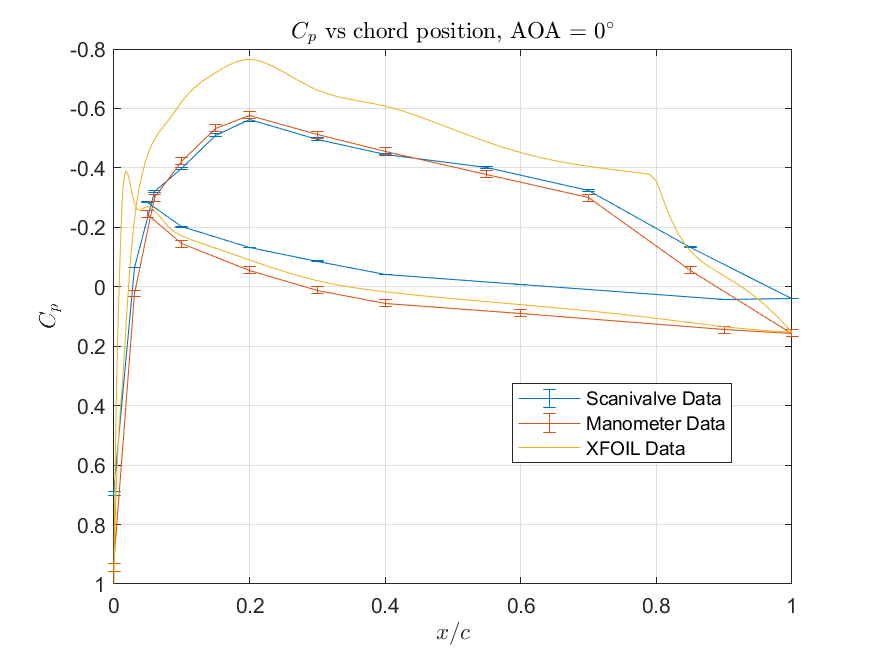
\includegraphics[width=\textwidth]{figures/AOA0.png}
        \caption{$C_p$ distribution at $\alpha = 0^\circ$}
        \label{fig:cp_0}
    \end{subfigure}
    \begin{subfigure}[b]{0.3\textwidth}
        \centering
        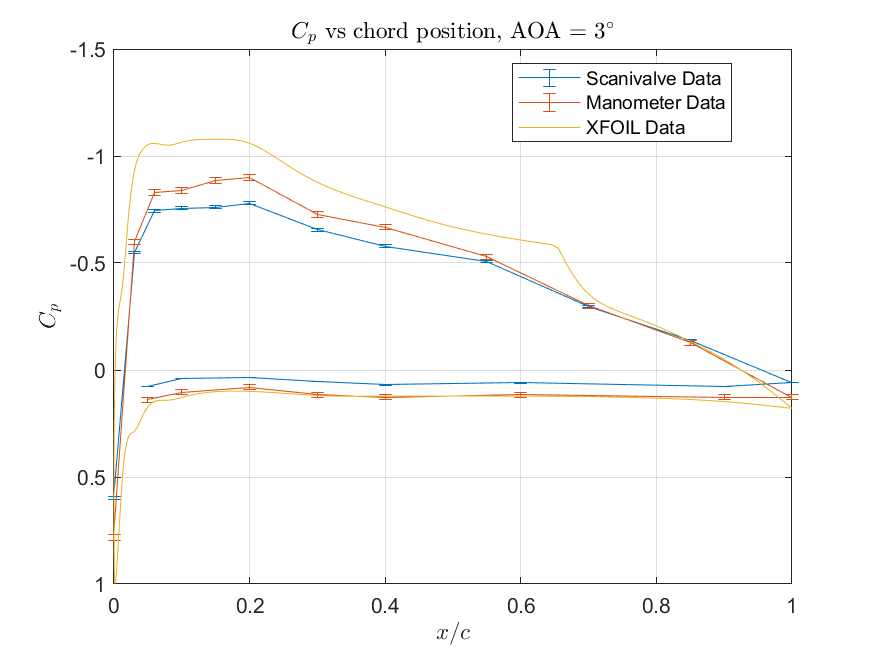
\includegraphics[width=\textwidth]{figures/AOA3.png}
        \caption{$C_p$ distribution at $\alpha = 3^\circ$}
        \label{fig:cp_3}
    \end{subfigure}
    \begin{subfigure}[b]{0.3\textwidth}
        \centering
        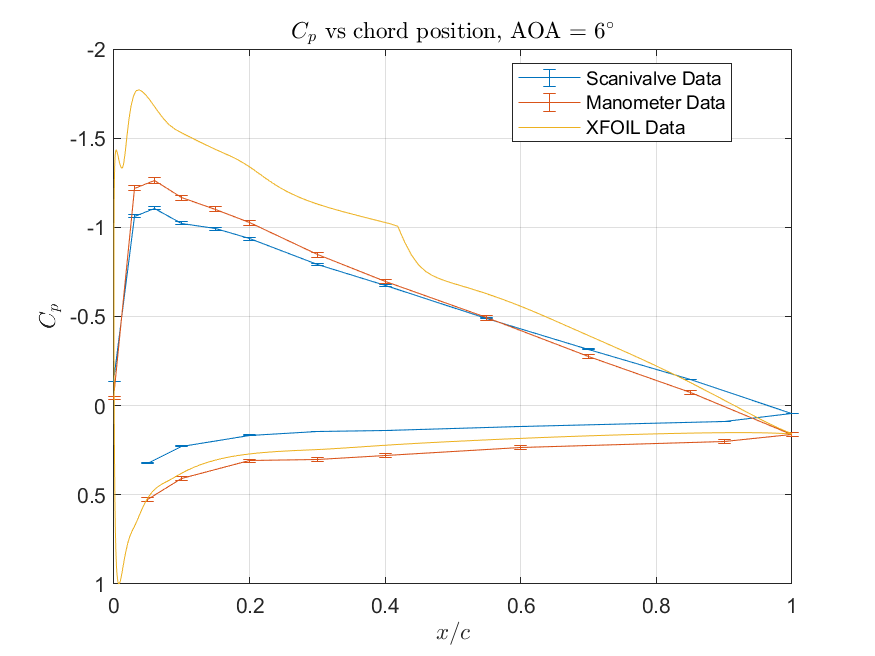
\includegraphics[width=\textwidth]{figures/AOA6.png}
        \caption{$C_p$ distribution at $\alpha = 6^\circ$}
        \label{fig:cp_6}
    \end{subfigure}
    \begin{subfigure}[b]{0.3\textwidth}
        \centering
        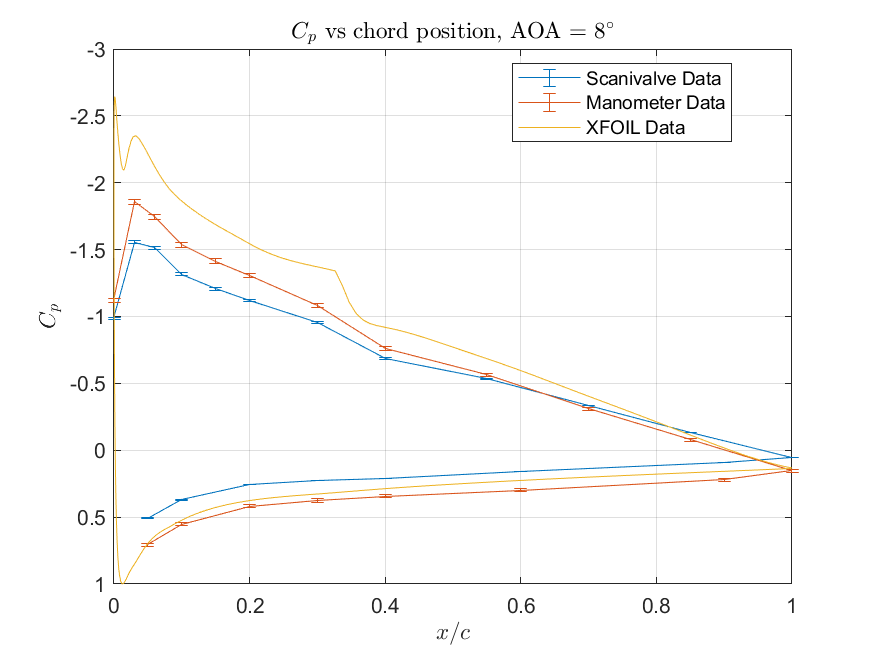
\includegraphics[width=\textwidth]{figures/AOA8.png}
        \caption{$C_p$ distribution at $\alpha = 8^\circ$}
        \label{fig:cp_8}
    \end{subfigure}
    \begin{subfigure}[b]{0.3\textwidth}
        \centering
        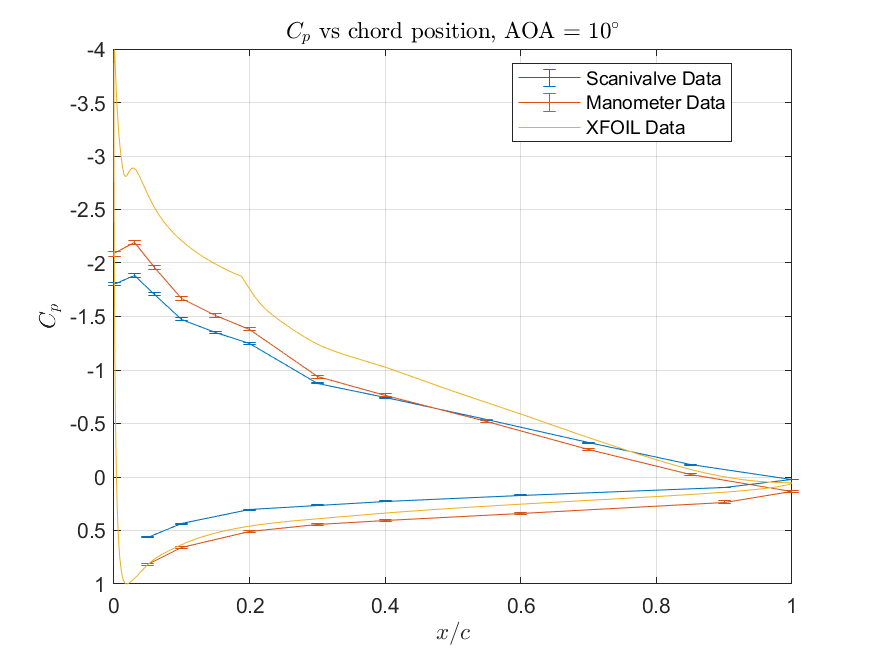
\includegraphics[width=\textwidth]{figures/AOA10.png}
        \caption{$C_p$ distribution at $\alpha = 10^\circ$}
        \label{fig:cp_10}
    \end{subfigure}
    \begin{subfigure}[b]{0.3\textwidth}
        \centering
        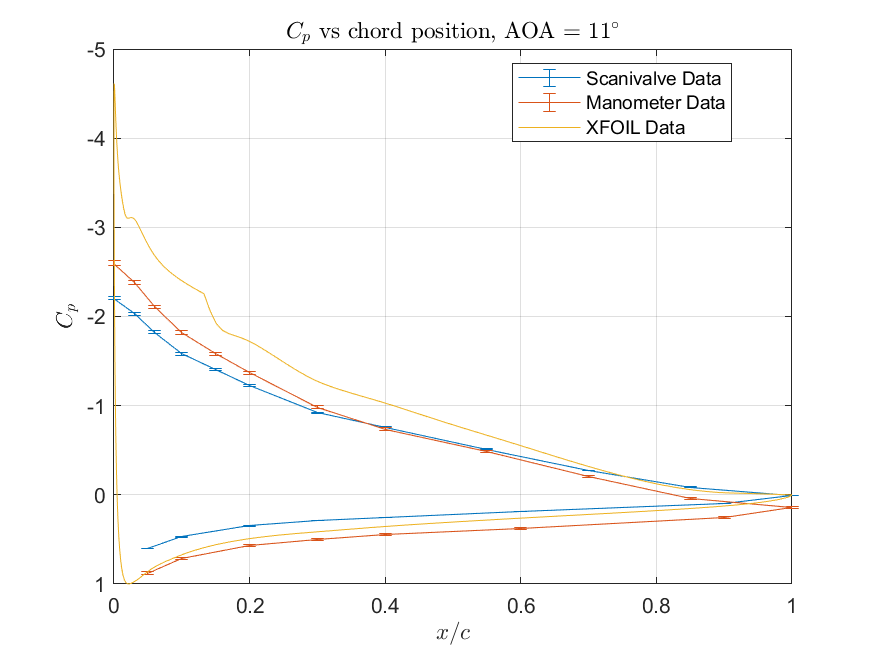
\includegraphics[width=\textwidth]{figures/AOA11.png}
        \caption{$C_p$ distribution at $\alpha = 11^\circ$}
        \label{fig:cp_11}
    \end{subfigure}
    \begin{subfigure}[b]{0.3\textwidth}
        \centering
        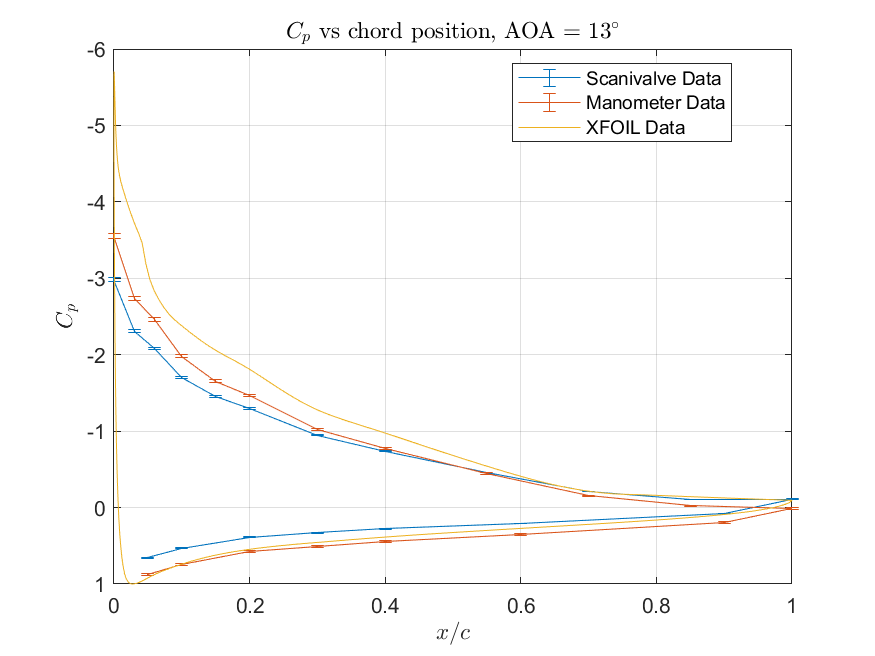
\includegraphics[width=\textwidth]{figures/AOA13.png}
        \caption{$C_p$ distribution at $\alpha = 13^\circ$}
        \label{fig:cp_13}
    \end{subfigure}
    \begin{subfigure}[b]{0.3\textwidth}
        \centering
        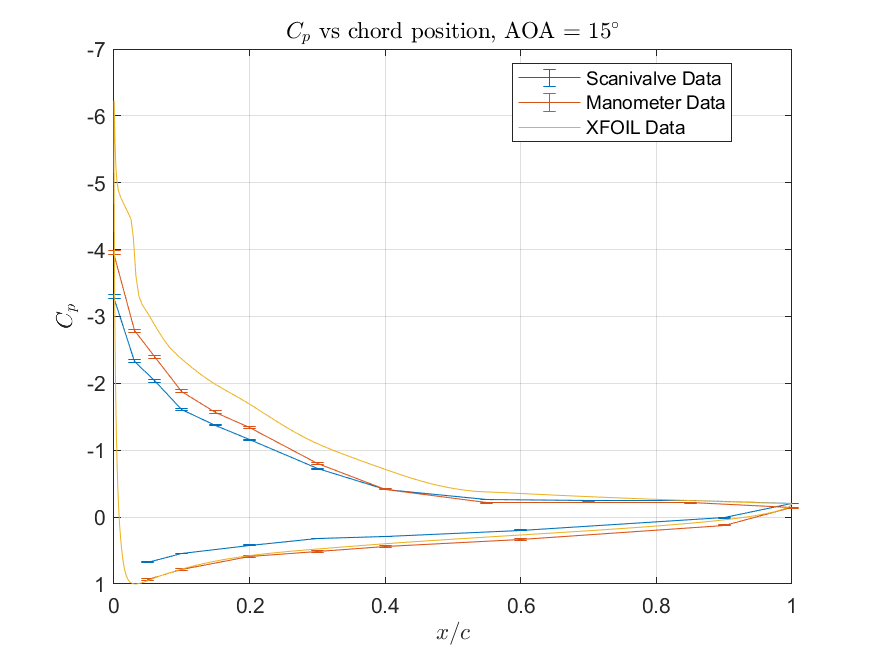
\includegraphics[width=\textwidth]{figures/AOA15.png}
        \caption{$C_p$ distribution at $\alpha = 15^\circ$}
        \label{fig:cp_15}
    \end{subfigure}
    \begin{subfigure}[b]{0.3\textwidth}
        \centering
        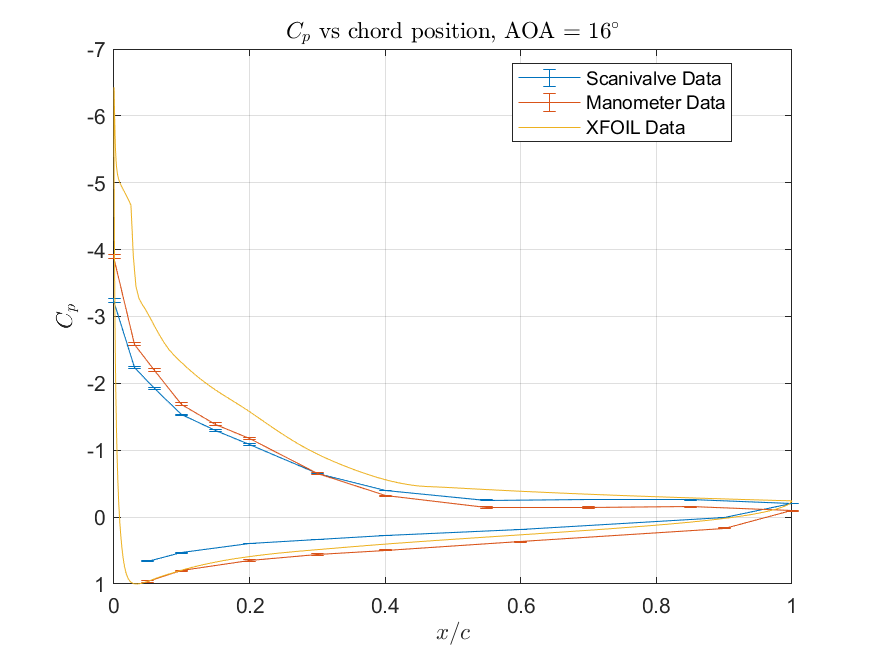
\includegraphics[width=\textwidth]{figures/AOA16.png}
        \caption{$C_p$ distribution at $\alpha = 16^\circ$}
        \label{fig:cp_16}
    \end{subfigure}
    \begin{subfigure}[b]{0.3\textwidth}
        \centering
        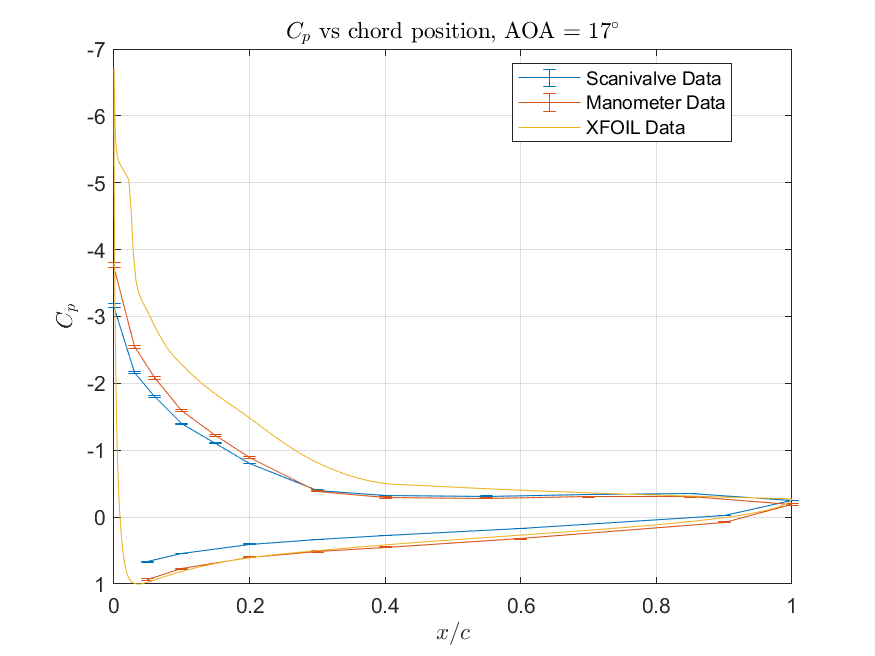
\includegraphics[width=\textwidth]{figures/AOA17.png}
        \caption{$C_p$ distribution at $\alpha = 17^\circ$}
        \label{fig:cp_17}
    \end{subfigure}
    \begin{subfigure}[b]{0.3\textwidth}
        \centering
        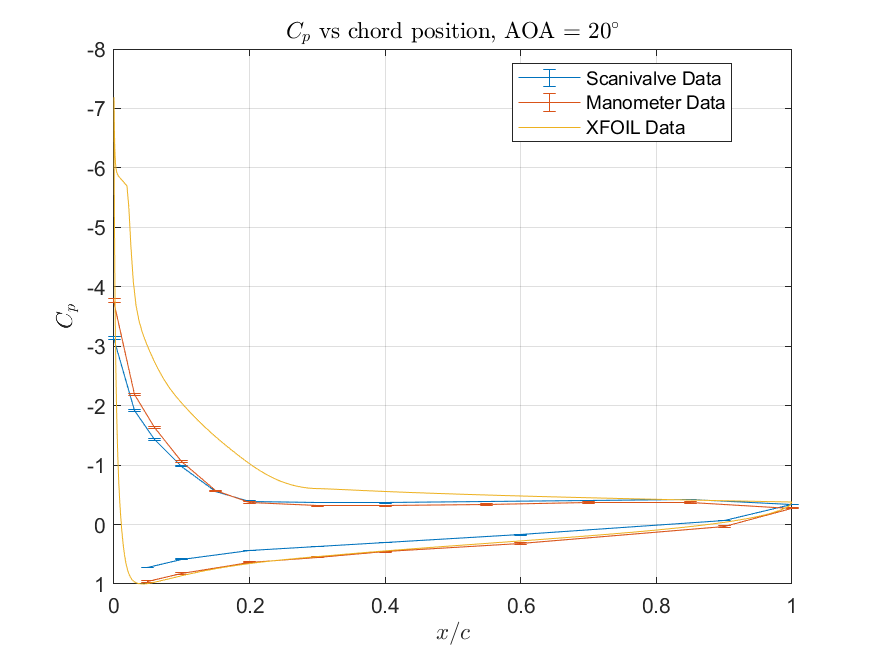
\includegraphics[width=\textwidth]{figures/AOA20.png}
        \caption{$C_p$ distribution at $\alpha = 20^\circ$}
        \label{fig:cp_20}
    \end{subfigure}
    \caption{$C_p$ distribution of all angles of attack.}
    \label{fig:cp}
\end{figure}

\noindent
Overall, the trend of the $C_p$ distribution fits the theoretical prediction. The upper wing has a more negative pressure distribution than the lower wing, which in turn provides lift. The $C_p$ changes drastically in the small region directly succeeding the leading edge due to the static pressure. The upper surface of the airfoil has a negative pressure peak around the leading edge, whose magnitude is directly proportional to the angle of attack.For lower angles of attack, the $C_p$ changes gradually after the leading edge, but for higher angles of attack, due to viscous effects, a pressure plateau becomes significant for $\alpha \ge 13^\circ$, which is associated with the stalling of the airfoil.\newline 

\noindent
The plateau of the upper airfoil surface $C_p$ distribution reduces the pressure gradient between the top and bottom airfoil surfaces, which results in a loss of lift. Aircraft designers must consider stalling effects, and optimize the stall angles. Pilots also should be reminded about stall angles to prevent accidents during flight (specifically when making abrupt pitching actions).\newline

\noindent
The general pattern of the $C_p$ distribution, as well as the stall angle is verified with XFOIL. Experimental results deviate slightly at the leading edge with XFOIL, which likely originates from the assumptions XFOIL employs (despite having a separate viscous solver). Such errors between representations can alert aerodynamicists where a model differs from real life thereby highlighting where experiments must be conducted in order to see the full picture. Furthermore, the $C_p$ distribution is consistent with the literature\cite{lyon_broeren_giguere_gopalarathnam_selig_1997} which reports the $C_p$ distribution as seen in figure \ref{fig:lit_cp} and agrees with the overall pattern seen in the experiment.

\begin{figure}[h]
    \centering
    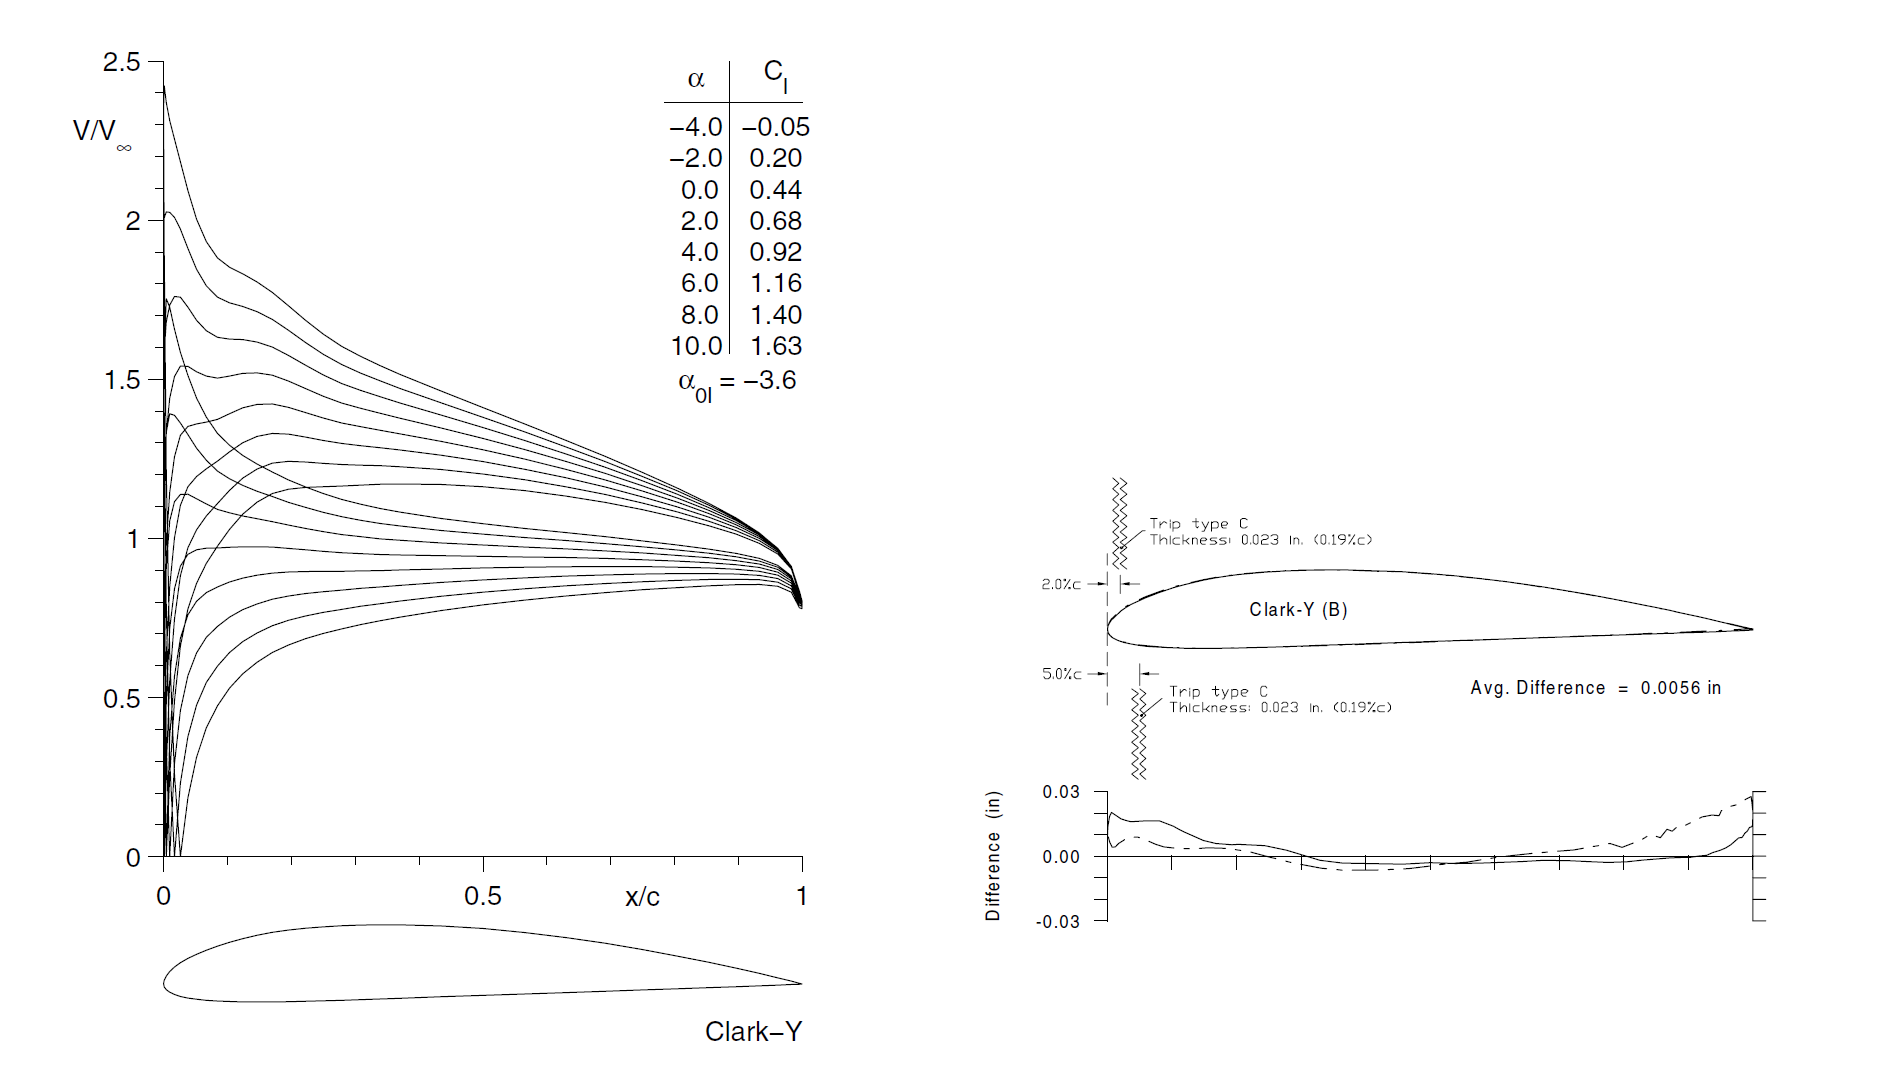
\includegraphics[width=\textwidth]{figures/reference_cp.png}
    \caption{Reference $C_p$ distribution with various AOA.}
    \label{fig:lit_cp}
\end{figure}

\subsection{Wake Velocity Profile}

\noindent
Wake velocities are obtained from total pressure measurements in the wake to determine the flow velocity distribution over the height of the pressure rake. Resulting total drag is computed numericall using equation \ref{fig:total_drag_coefficient} and \verb|trapz| in MATLAB. The drag coefficient $C_D$ is obtained using equation \ref{eq:cd}. Wake velocity and $C_D$ results are shown in Figures \ref{fig:wake_velocities} and \ref{fig:total_drag_coefficient}.\newline

\noindent
The shape of the wake velocity distributions are consistent with theory, indicating that the airfoil only disturbs flow near it, and that the velocity profile going off to infinity approaches the freestream velocity. It should be noted that the wake velocity profiles, especially for $\alpha$ near and around stall, exhibit time-varying effects such as vortex shedding not captured by the static measurements of this experiment. The large jagged fluctuations in the observed data are artifacts of the measurement process. The wake velocity distributions should be collected using a time-averaging method of many measurements over a long period of time if the experiment were to be repeated with more time allotted.\newline

\noindent
In both sets of plots, a dramatic change occurs between $\alpha = 13^\circ$ and $\alpha = 15 ^\circ$. The peak velocity deficit increases in magnitude, and shifts downward in position. The downwards movement of the peak is due to the increasing angle of attack deflecting more flow downward, and is not related to stall. The dramatically large peak is indicative of stall as separated flow produces much more drag than well-attached flow. Additionally, the $C_D$ jumps up dramatically between $\alpha = 13^\circ$ and $\alpha = 15 ^\circ$. This is indicative of stall occurring and producing more drag. Based on these measurements, the stall angle appears to be about $13^\circ$.\newline

\noindent
Both sets of measurements agree with XFOIL in terms of predicting stall angle, as well as the general shape of the $C_D$ curve. Error bars overlap the simulation data for most of the datapoints, suggesting good measurements and a good estimation of error. The manometer error bars are larger than those of the scanivalve, due to many sources of error in the scanivalve not being accounted for.\newline

\begin{figure}
    \centering
    \begin{subfigure}[b]{0.45\textwidth}
         \centering
         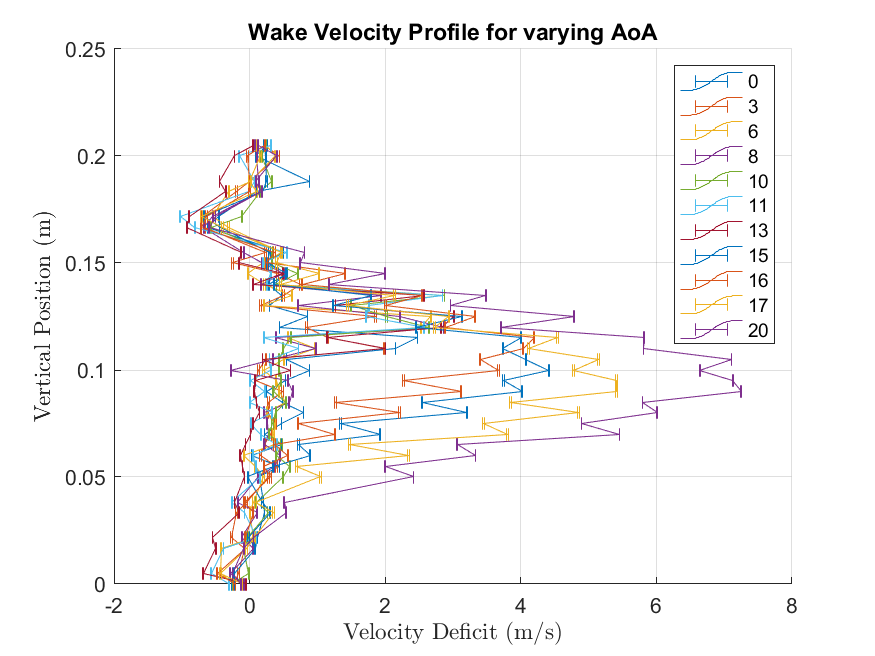
\includegraphics[width=\textwidth]{figures/scanivalve_wake_velocities.png}
          \caption{Scanivalve wake deficit.}
         \label{fig:scanivalve_wake_velocity}
     \end{subfigure}
     \begin{subfigure}[b]{0.45\textwidth}
         \centering
         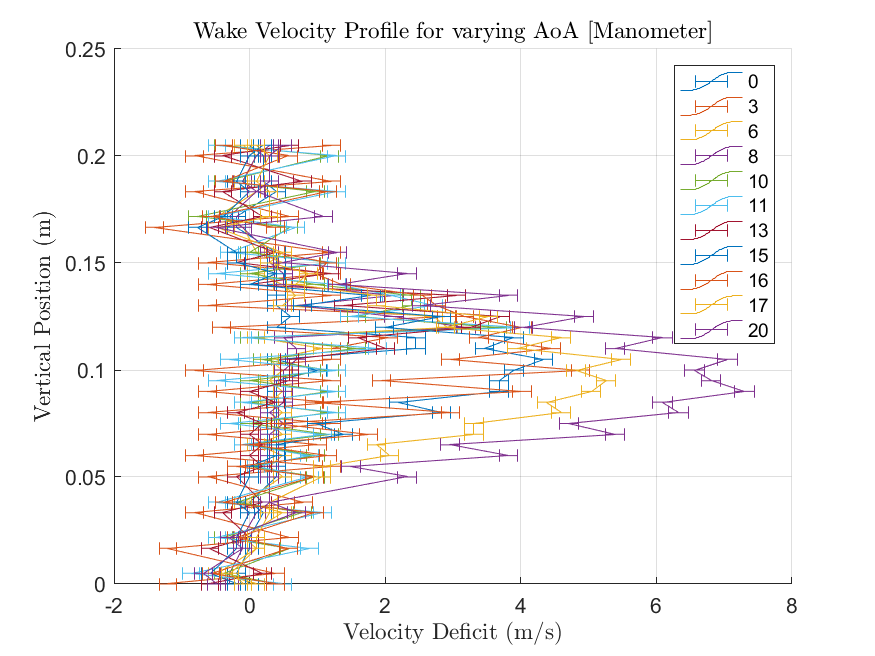
\includegraphics[width=\textwidth]{figures/manometer_wake_velocities.png}
         \caption{Manometer wake deficit.}
         \label{fig:manometer_wake_velocity}
     \end{subfigure}
    \caption{Velocity deficit, $U_\infty - u$, in the wake for each $\alpha$, from both the scanivalve and manometer data.}
    \label{fig:wake_velocities}
\end{figure}

\begin{figure}
    \centering
    \begin{subfigure}[b]{0.45\textwidth}
         \centering
         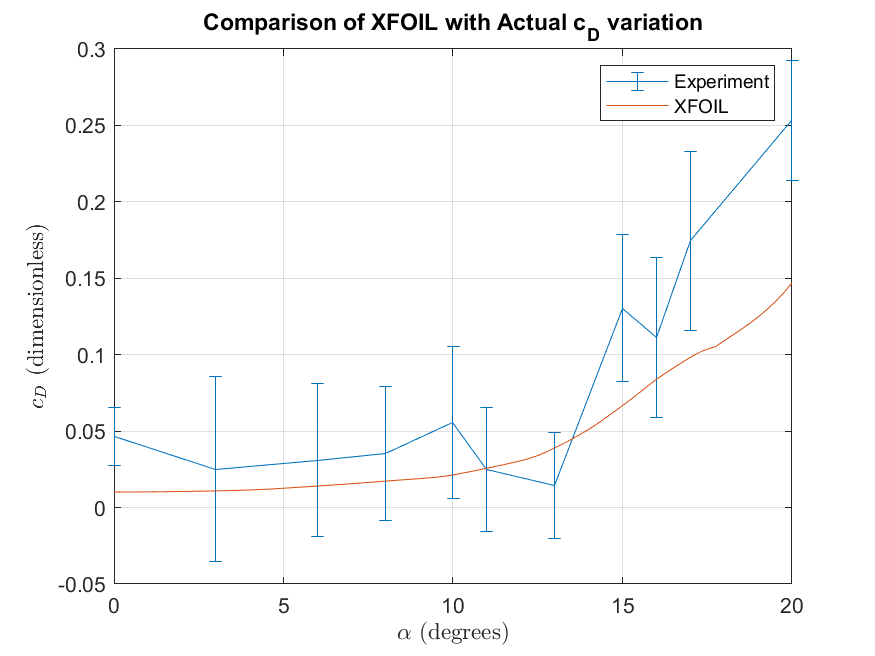
\includegraphics[width=\textwidth]{figures/scanivalve_cd.png}
         \caption{}
         \label{fig:scanivalve_drag_coef}
     \end{subfigure}
     \begin{subfigure}[b]{0.45\textwidth}
         \centering
         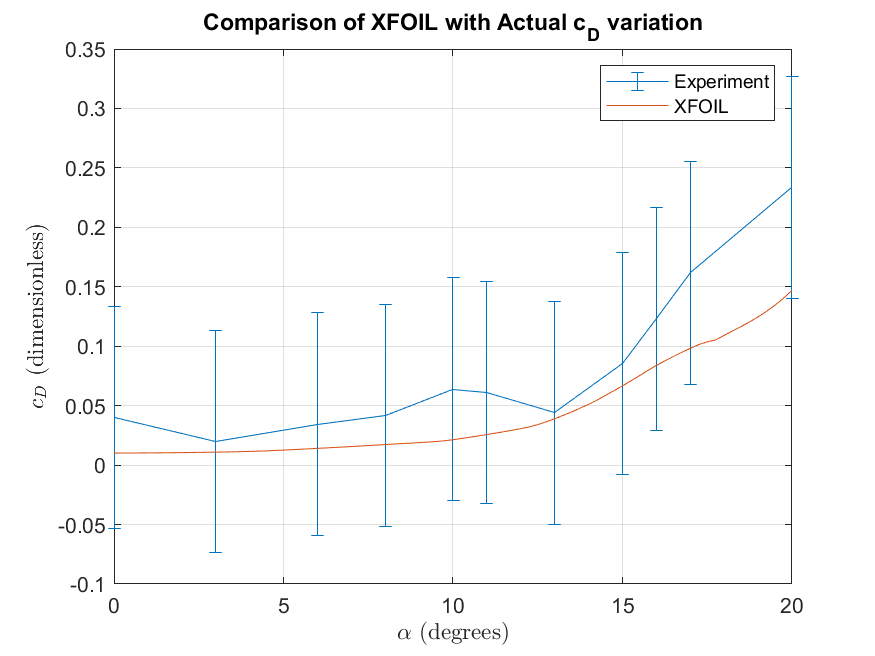
\includegraphics[width=\textwidth]{figures/manometer_cd.png}
         \caption{}
         \label{fig:manometer_drag_coef}
     \end{subfigure}
    \caption{Total drag coefficient versus XFOIL.}
    \label{fig:total_drag_coefficient}
\end{figure}

\subsection{Coefficient of Lift, Pressure Drag, and Moment}

\begin{figure}
    \centering
    \begin{subfigure}[b]{0.45\textwidth}
         \centering
         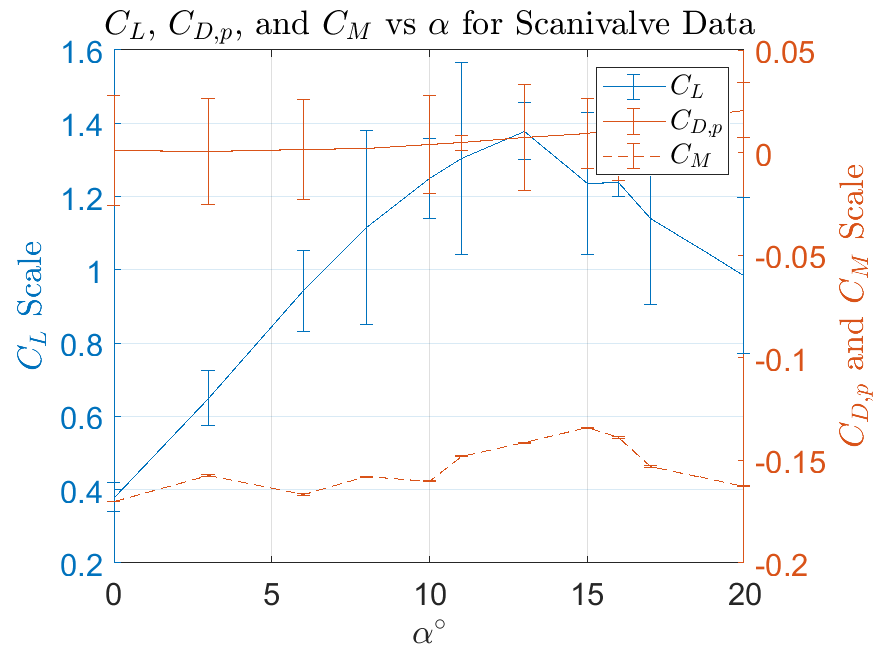
\includegraphics[width=\textwidth]{figures/scanivalve_cl_cd_cm.png}
         \caption{Coefficients calculated from scanivalve data.}
         \label{fig:scani_coeff}
     \end{subfigure}
     \begin{subfigure}[b]{0.45\textwidth}
         \centering
         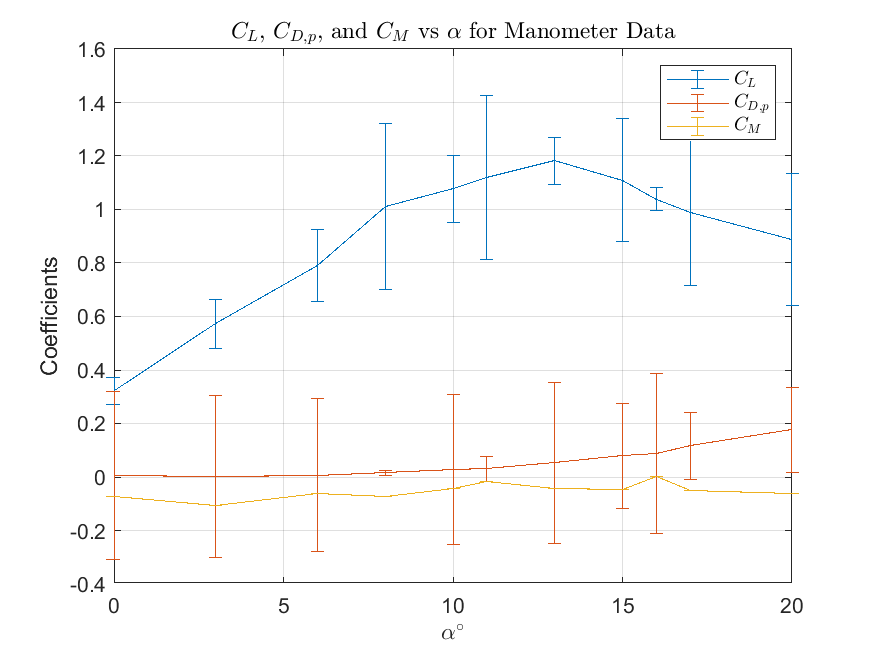
\includegraphics[width=\textwidth]{figures/manometer_cl_cd_cm.png}
         \caption{Coefficients calculated from manometer data.}
         \label{fig:mano_coeff}
     \end{subfigure}
    \caption{Empirically determined coefficients of lift, pressure drag, and moment.}
    \label{fig:coeffs}
\end{figure}

\noindent
Both the scanivalve and manometer data were calibrated and then processed according to the methods detailed in section \ref{sec:procedure} to yield the lift, (pressure) drag, and  moment coefficients for the Clark Y airfoil. The coefficient relationship with the angle of attack is displayed pictorially in figures \ref{fig:scani_coeff} and \ref{fig:mano_coeff} as well as in tabular form in tables \ref{tab:scani_coeff} and \ref{tab:mano_coeff}.\newline

\begin{table}[h]
\centering
\begin{tabular}{p{3cm}p{3cm}p{3cm}p{3cm}}
    % THE FOLLOWING IS THE PRE-SKETCHY TABLE
% \toprule
% $\alpha^\circ$ & $C_L$ & $C_{D,p}$ & $C_M$ \\
% \midrule
%  $0.00\pm0.25$ & $0.380\pm0.039$ & $0.0100236\pm0.27$ &  $-0.170094\pm0.000050$ \\
%  $3.00\pm0.25$ & $0.650\pm0.076$ & $0.01\pm0.26$ & $-0.15733\pm0.00051$ \\
%  $6.00\pm0.25$ & $0.94\pm0.11$ & $0.01\pm0.24$ &  $-0.16652\pm0.00035$ \\
%  $8.00\pm0.25$ & $1.12\pm0.26$ &  $0.02068\pm0.00082$ & $-0.15797\pm0.00026$ \\
% $10.00\pm0.25$ & $1.25\pm0.11$ & $0.04\pm0.24$ & $-0.16007\pm0.00033$ \\
% $11.00\pm0.25$ & $1.30\pm0.26$ & $0.05\pm0.037$ &  $-0.14797\pm0.00022$ \\
% $13.00\pm0.25$ & $1.379\pm0.077$ &  $0.07\pm0.26$ & $-0.14144\pm0.00016$ \\
% $15.00\pm0.25$ & $1.24\pm0.19$ & $0.09\pm0.17$ & $-0.13417\pm0.00032$ \\
% $16.00\pm0.25$ & $1.238\pm0.038$ & $0.12\pm0.26$ & $-0.13876\pm0.00037$ \\
% $17.00\pm0.25$ &  $1.14\pm0.23$ & $0.14\pm0.11$ &  $-0.15305\pm0.00048$ \\
% $20.00\pm0.25$ & $0.99\pm0.21$ &  $0.21\pm0.13$ & $-0.16259\pm0.00021$ \\
% \bottomrule
% \end{tabular}
\toprule
$\alpha^\circ$ &                   $C_L$ &               $C_{D,p}$ &                    $C_M$ \\
\midrule
 $0.00\pm0.25$ & $0.380\pm0.039$ & $0.001\pm0.027$ &  $-0.170094\pm0.000050$ \\
 $3.00\pm0.25$ & $0.650\pm0.076$ & $0.001\pm0.026$ & $-0.15733\pm0.00051$ \\
 $6.00\pm0.25$ & $0.94\pm0.11$ & $0.001\pm0.024$ &  $-0.16652\pm0.00035$ \\
 $8.00\pm0.25$ & $1.12\pm0.26$ &  $0.002068\pm0.000082$ & $-0.15797\pm0.00026$ \\
$10.00\pm0.25$ & $1.25\pm0.11$ & $0.004\pm0.024$ & $-0.16007\pm0.00033$ \\
$11.00\pm0.25$ & $1.30\pm0.26$ &  $0.0047\pm0.0037$ &  $-0.14798\pm0.00022$ \\
$13.00\pm0.25$ & $1.379\pm0.077$ & $0.007\pm0.026$ & $-0.14144\pm0.00016$ \\
$15.00\pm0.25$ & $1.24\pm0.19$ & $0.009\pm0.017$ & $-0.13417\pm0.00032$ \\
$16.00\pm0.25$ & $1.238\pm0.038$ & $0.012\pm0.026$ & $-0.13876\pm0.00037$ \\
$17.00\pm0.25$ &  $1.14\pm0.23$ & $0.014\pm0.011$ &  $-0.15305\pm0.00048$ \\
$20.00\pm0.25$ & $0.99\pm0.21$ & $0.021\pm0.013$ & $-0.16259\pm0.00021$ \\
\bottomrule
\end{tabular}
\caption{Coefficients of lift, pressure drag, and moment for the scanivalve data.}
\label{tab:scani_coeff}
\end{table}

\begin{table}[h]
\centering
\begin{tabular}{p{3cm}p{3cm}p{3cm}p{3cm}}
% THE FOLLOWING IS THE PRE-SKETCHY TABLE
% \toprule
% $\alpha^\circ$ & $C_L$ & $C_{D,p}$ & $C_M$ \\
% \midrule
%  $0.00\pm0.25$ & $0.322\pm0.050$ & $0.01\pm0.32$ &  $-0.072506\pm0.000050$ \\
%  $3.00\pm0.25$ & $0.573\pm0.092$ &   $0.00\pm0.30$ & $-0.10605\pm0.00051$ \\
%  $6.00\pm0.25$ & $0.79\pm0.13$ &  $0.0074\pm0.28$ &  $-0.06257\pm0.00035$ \\
%  $8.00\pm0.25$ & $1.01\pm0.31$ & $0.0153\pm0.0086$ & $-0.071424\pm0.00026$ \\
% $10.00\pm0.25$ & $1.08\pm0.13$ & $0.03\pm0.28$ & $-0.04364\pm0.00033$ \\
% $11.00\pm0.25$ & $1.12\pm0.31$ & $0.032\pm0.047$ & $-0.01843\pm0.00022$ \\
% $13.00\pm0.25$ & $1.181\pm0.087$ &  $0.05\pm0.30$ & $-0.04153\pm0.00016$ \\
% $15.00\pm0.25$ & $1.11\pm0.23$ & $0.08\pm0.20$ & $-0.04825\pm0.00032$ \\
% $16.00\pm0.25$ & $1.038\pm0.042$ & $0.09\pm0.30$ &  $0.00178\pm0.00037$ \\
% $17.00\pm0.25$ & $0.99\pm0.27$ & $0.12\pm0.13$ &  $-0.05075\pm0.00048$ \\
% $20.00\pm0.25$ & $0.89\pm0.25$ & $0.18\pm0.16$ & $-0.06027\pm0.00021$ \\
% \bottomrule
% \end{tabular}
\toprule
$\alpha^\circ$ & $C_L$ & $C_{D,p}$ & $C_M$ \\
\midrule
 $0.00\pm0.25$ & $0.322\pm0.050$ &  $0.001\pm0.032$ &  $-0.072506\pm0.000050$ \\
 $3.00\pm0.25$ & $0.573\pm0.092$ &  $0.000\pm0.030$ & $-0.10605\pm0.00051$ \\
 $6.00\pm0.25$ & $0.792\pm0.13$ & $0.001\pm0.028$ &  $-0.06257\pm0.00035$ \\
 $8.00\pm0.25$ & $1.01\pm0.31$ & $0.00153\pm0.00085$ & $-0.07142\pm0.00026$ \\
$10.00\pm0.25$ & $1.08\pm0.13$ & $0.0027\pm0.028$ & $-0.04364\pm0.00033$ \\
$11.00\pm0.25$ & $1.12\pm0.31$ & $0.0032\pm0.0047$ & $-0.01843\pm0.00022$ \\
$13.00\pm0.25$ & $1.181\pm0.087$ &  $0.005\pm0.030$ & $-0.04153\pm0.00016$ \\
$15.00\pm0.25$ & $1.11\pm0.23$ & $0.008\pm0.020$ & $-0.04825\pm0.00032$ \\
$16.00\pm0.25$ & $1.038\pm0.042$ & $0.009\pm0.030$ &  $0.00178\pm0.00037$ \\
$17.00\pm0.25$ & $0.99\pm0.27$ & $0.012\pm0.013$ &  $-0.05075\pm0.00048$ \\
$20.00\pm0.25$ & $0.89\pm0.25$ & $0.018\pm0.016$ & $-0.06027\pm0.00021$ \\
\bottomrule
\end{tabular}
\caption{Coefficients of lift, pressure drag, and moment for the manometer data.}
\label{tab:mano_coeff}
\end{table}

\noindent
In both plots, the coefficient of lift increases with the angle of attack until $\alpha\approx13^\circ$ at which the coefficient of lift begins decreasing for all higher angles of attack. There are various features within the lift curve to discuss.

\begin{itemize}

    \item The first feature to discuss is the non-zero coefficient of lift produced at $\alpha=0^\circ$. This signifies a degree of camber inherent to the airfoil indicating that the Clark Y airfoil is not symmetric which is in line with our understanding.
    
    \item A linear $C_L$-$\alpha$ dependency exists for angles of attack within the approximate range from $0^\circ$ to $8^\circ$. This region is characterized by a very minimal boundary layer that does not significantly hinder lift production.
    
    \item For the approximate range from $8^\circ$ to $13^\circ$, there is a diminishing lift slope. As the angle of attack increases, the point of separation moves forward on the leading edge as seen by the beginning of the plateau on the $C_p$ plots in figure \ref{fig:cp}. The growing boundary layer inhibits lift production thereby reducing the rate of $C_L$ increase.
    
    \item For $\alpha\approx13^\circ$, we have the critical angle of attack (where $C_L$ is a maximum) where the increased flow separation dominates causing diminishing lift. The critical angle of attack is a significant characteristic of an airfoil as it sets a lower bound on the speed at which an aircraft can fly. As an aircraft slows down, a higher angle of attack is necessary to produce sufficient lift to counterbalance the aircraft's weight. Although increasing the angle of attack, as seen in the $C_L$ plots will only be met with increasing lift until this critical angle is met at which the aircraft can no longer sustain flight.
    
    \item For the remainder of the $C_L$ curve, increasing the angle of attack emphasizes the domination of flow separation and the continual decrease in lift production.
\end{itemize}

\noindent
The coefficient of drag plots decrease initially but as they begin nearing the critical angle of attack, they begin to increase indicating an increased pressure drag force applied to the airfoil. The increasing nature of the $C_{D,p}$ curve around and past the critical angle is due to the increasing boundary layer thickness which results in higher viscous effects and consequently more drag experienced.\newline

\noindent
Lastly, the coefficient of moment curves follow a behaviour that is weakly inverse to that of the (pressure) drag coefficient where it increases with an increasing angle of attack until the critical angle is reached before becoming more negative with a further increase in the angle of attack. With this in mind, the general trend of the $C_M$ curve weak and no significant results can be extracted. This result vaguely resembles the trends of XFOIL but are in line with the literature which describes the $C_M$ curve becoming positive at the onset of a stall. These discrepancies could be the result of experimental error or analysis error and deem further investigation. \newline

\noindent
The coefficients calculated from the experimental data can be compared to the results from XFOIL as seen in figures \ref{fig:scani_comp} and \ref{fig:mano_comp} for the Scanivalve and manometer data respectively.\newline

\noindent
The experimental results are a better match for the $C_L$ and $C_D$ curve for the scanivalve data where the majority of the XFOIL data falls within the uncertainty of the experimental data. Since the experimental procedure did not calculate viscous effects, the experimental $C_D$ curve begins to deviate from the XFOIL $C_D$ curve at higher angles of attack when viscous effects become significant. XFOIL's viscous solver makes it a more accurate descriptor of the real flow in high viscous conditions. \newline

\noindent
For the manometer data, there is a larger deviation between the lift and drag coefficient curves compared to the XFOIL data. These discrepancies are emphasized by the greater sources of error associated with manometer measurements described in section \ref{sec:source_of_error}. The relationships between the lift and drag coefficient curves for the manometer data compared to the XFOIL data are similar to that of the scanivalve-to-XFOIL relationships stated earlier.

\begin{figure}[h]
    \centering
    \begin{subfigure}[b]{0.45\textwidth}
         \centering
         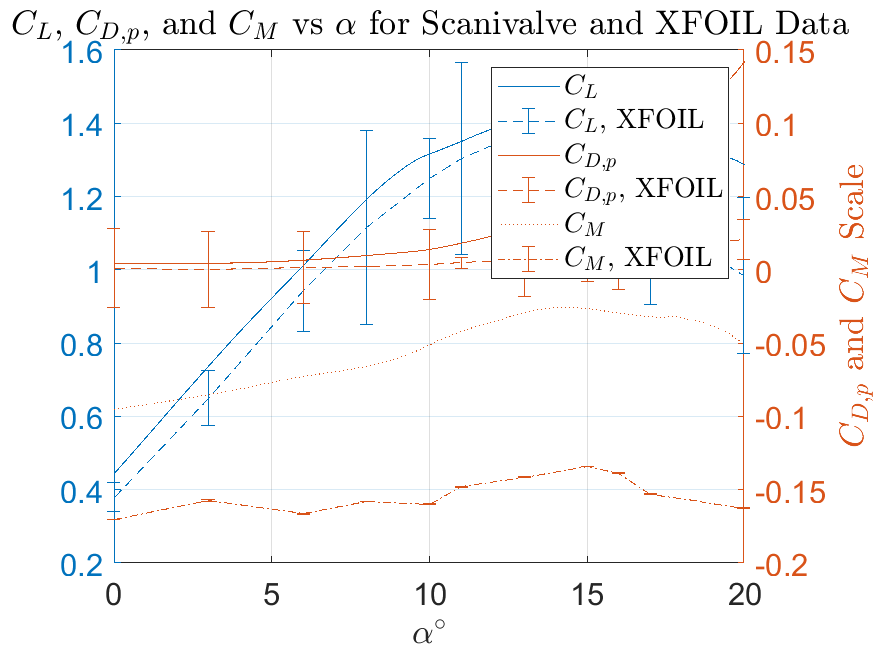
\includegraphics[width=\textwidth]{figures/scanivalve_XFOIL_cl_vs_cd.png}
         \caption{$C_L$, $C_{D,p}$, and $C_M$ scanivalve data compared to XFOIL.}
         \label{fig:scani_comp}
     \end{subfigure}
     \begin{subfigure}[b]{0.45\textwidth}
         \centering
         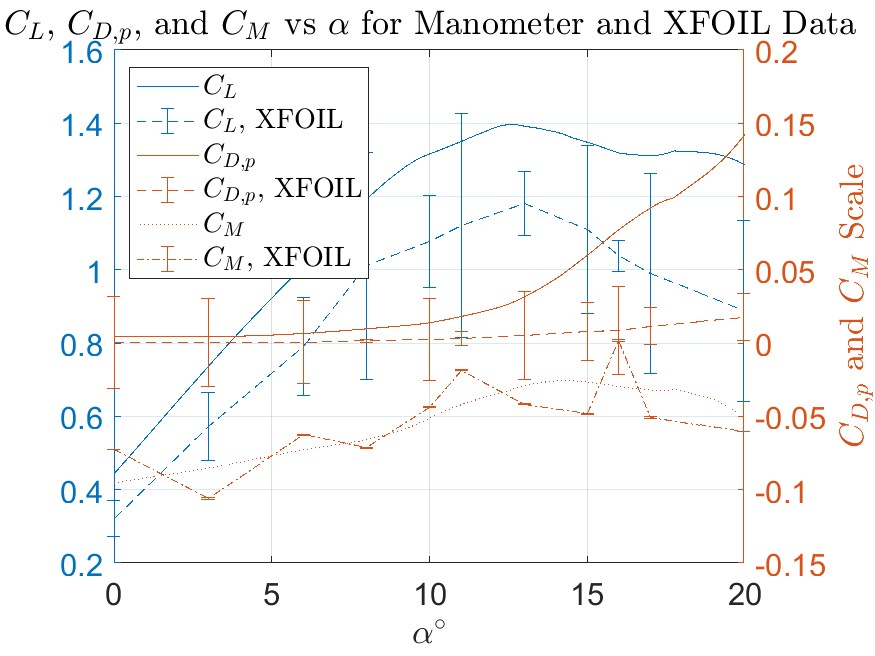
\includegraphics[width=\textwidth]{figures/manometer_XFOIL_cl_vs_cd.png}
         \caption{$C_L$, $C_{D,p}$, and $C_M$ manometer data compared to XFOIL.}
         \label{fig:mano_comp}
     \end{subfigure}
    \caption{Comparing $C_L$, $C_{D,p}$, and $C_M$ curves to XFOIL.}
    \label{fig:curve_comp}
\end{figure}

\begin{figure}[h]
    \centering
    \begin{subfigure}[b]{0.45\textwidth}
         \centering
         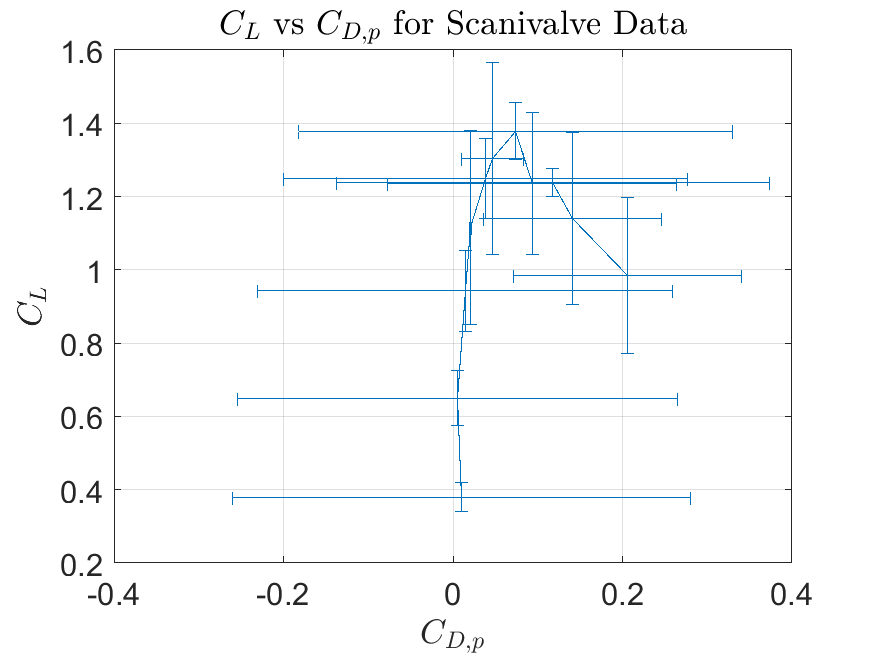
\includegraphics[width=\textwidth]{figures/scanivalve_cl_vs_cd.png}
         \caption{$C_L$ vs $C_{D,p}$ from scanivalve data.}
         \label{fig:scani_cL_cD}
     \end{subfigure}
     \begin{subfigure}[b]{0.45\textwidth}
         \centering
         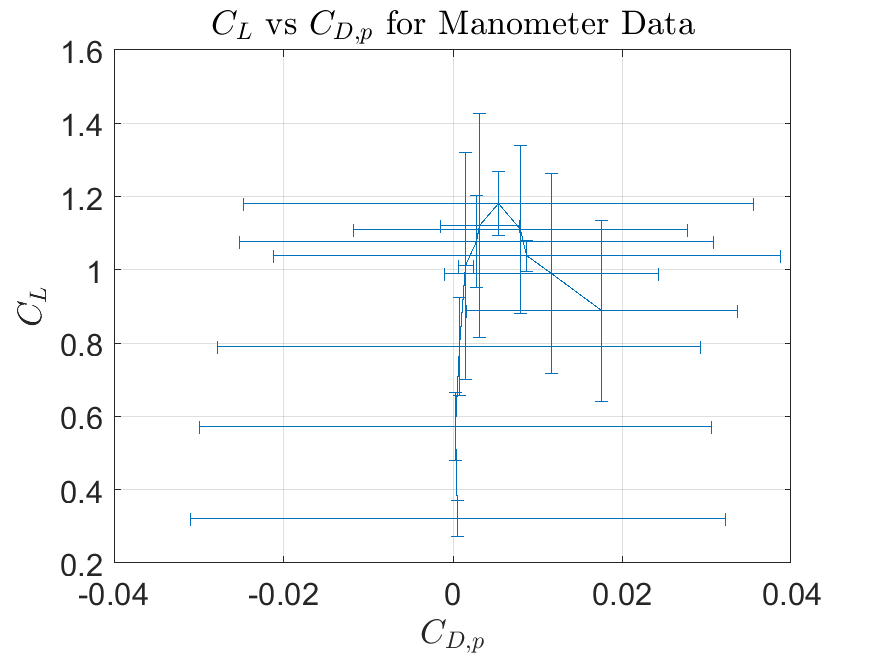
\includegraphics[width=\textwidth]{figures/manometer_cl_vs_cd.png}
         \caption{$C_L$ vs $C_{D,p}$ from manometer data.}
         \label{fig:mano_cL_cD}
     \end{subfigure}
    \caption{Empirically determined $C_L$ vs $C_{D,p}$ curves.}
    \label{fig:cL_vs_cD}
\end{figure}

\noindent
Experimental performance data of a Clark Y airfoil is available in literature
\cite{lyon_broeren_giguere_gopalarathnam_selig_1997}. The relevant plots on page 81 and 83 give experimental results for dimensionless coefficients measured in a more professional manner. These are shown in Figure \ref{fig:clark_y_reference}.\newline

\noindent
The shape of the $C_L$ vs $\alpha$ plot in Figure \ref{fig:coeffs} agrees well with the reference experiment in terms of stall angle, as well as the plateau behaviour around 10 degrees.

\begin{figure}[h]
    \centering
    \begin{subfigure}[b]{0.45\textwidth}
         \centering
         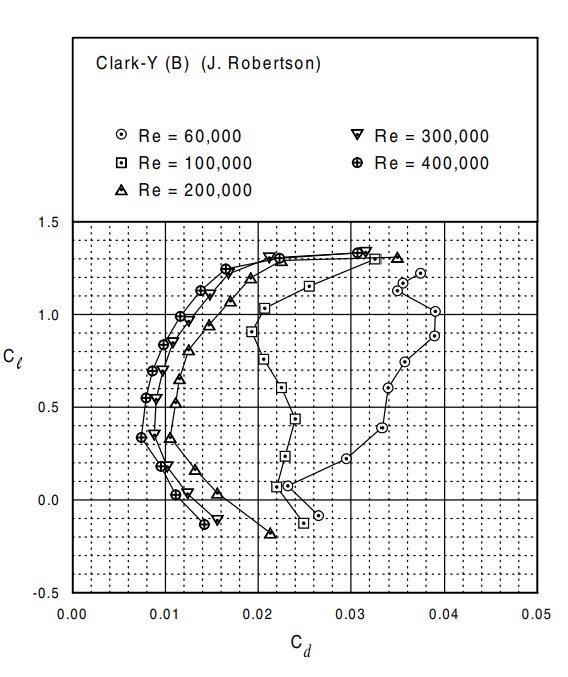
\includegraphics[width=\textwidth]{figures/clark_y_reference_cl_cd.jpg}
         \caption{}
         \label{fig:reference_cl_cd}
     \end{subfigure}
     \begin{subfigure}[b]{0.45\textwidth}
         \centering
         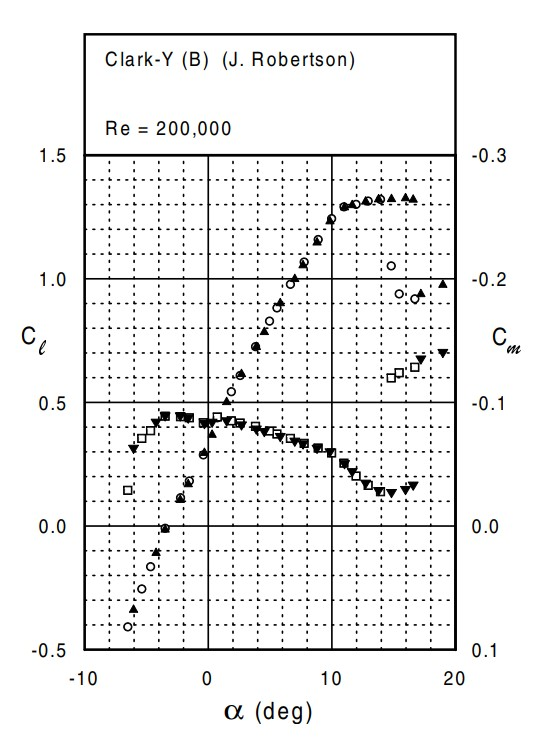
\includegraphics[width=\textwidth]{figures/clark_y_reference_cl_cm.jpg}
         \caption{}
         \label{fig:reference_cl_cm}
     \end{subfigure}
    \caption{Reference data for the Clark Y airfoil at $Re = 200000$.}
    \label{fig:clark_y_reference}
\end{figure}

\subsection{Pressure Drag and Total Drag Comparison}

\begin{table}[h]
\centering
\begin{tabular}{p{3cm}p{3cm}p{3cm}p{3cm}p{3cm}}
\toprule
$\alpha^\circ$ & $D'_p$ (Scanivalve) & $D'_p$ (Manometer) & $D'$ (Scanivalve) & $D'$ (Manometer) \\
\midrule
 $0.0\pm0.25$ &     $0.056\pm1.503$ &    $0.043\pm1.755$ &   $2.584\pm0.782$ &   $3.121\pm6.09$ \\
 $3.0\pm0.25$ &     $0.028\pm1.458$ &    $0.024\pm1.699$ &   $1.416\pm2.495$ &  $1.488\pm6.095$ \\
 $6.0\pm0.25$ &     $0.083\pm1.383$ &    $0.059\pm1.609$ &   $1.742\pm2.064$ &  $2.763\pm6.113$ \\
 $8.0\pm0.25$ &     $0.119\pm0.005$ &    $0.118\pm0.049$ &   $2.041\pm1.809$ &  $3.247\pm6.084$ \\
$10.0\pm0.25$ &     $0.223\pm1.379$ &     $0.221\pm1.62$ &   $3.222\pm2.052$ &  $5.152\pm6.061$ \\
$11.0\pm0.25$ &      $0.269\pm0.21$ &    $0.253\pm0.268$ &   $1.424\pm1.673$ &  $4.895\pm6.062$ \\
$13.0\pm0.25$ &     $0.419\pm1.455$ &    $0.425\pm1.707$ &   $0.821\pm1.425$ &  $3.468\pm6.076$ \\
$15.0\pm0.25$ &     $0.548\pm1.001$ &    $0.635\pm1.157$ &   $7.675\pm1.994$ &   $6.81\pm5.974$ \\
$16.0\pm0.25$ &     $0.694\pm1.502$ &    $0.724\pm1.759$ &   $6.537\pm2.159$ & $10.239\pm5.926$ \\
$17.0\pm0.25$ &     $0.832\pm0.622$ &    $0.951\pm0.745$ &  $10.323\pm2.421$ & $13.252\pm5.813$ \\
$20.0\pm0.25$ &     $1.242\pm0.811$ &    $1.379\pm0.965$ &  $15.284\pm1.619$ & $18.301\pm5.583$ \\
\bottomrule
\end{tabular}
\caption{Comparison of pressure and total drag force per unit span.}
\label{tab:pressure_comparison}
\end{table}

\noindent
Pressure drag makes up only a small portion of total drag for all measurements taken, consistent with theory from AER307 on airfoils at low speed. Total drag jumps sharply at stall $\alpha \approx 13^\circ$, indicative of a large viscous wake forming from separated flow. Pressure drag increases with $\alpha$ due to the airfoil itself pitching up. \newline

\noindent
The relative errors in the drag calculations are large, particularly for the pressure drag values. Therefore, trends observed in the pressure drag values are unreliable.


% -----------------------------------------------------------------------------
%   Sources of Error
% -----------------------------------------------------------------------------


\section{Sources of Error}\label{sec:source_of_error}

\subsection{Quantifiable Sources of Errors}
\begin{table}[H]
\begin{center}
    \begin{tabular}{ll}
        \toprule
        \multicolumn{2}{c}{Quantifiable Error}\\
        \midrule
        Manometer Uncertainty Reading & $\pm 1 \si{mm}$\\
        Manometer Angle Uncertainty & $\pm 0.5^\circ$ \\
        Angle of Attack Uncertainty & $\pm 0.25^\circ$ \\
        Scanivalve Precision & Acquired from autocorrelation using port 36 in each trial. See table (x)\\
        Scanivalve Bias & Assume to be 0 \\
        Calibration Coefficients & Assume to be 0\\
        \bottomrule
\end{tabular}
\end{center}
\caption{Quantifiable Sources of Error, Tabulated}
\label{tab:quant_error}
\end{table}

The precision error for the Scanivalve reading is acquired via an autocorrelation analysis. The autocorrelation formula is:
\begin{align}\label{eq:autocorrelation}
    T &= \int_{0}^{\infty} \frac{\overline{(x(t)-\bar{x})\cdot(x(t-\tau)-\bar{x})}}{\overline{(x(t) - \bar{x})^2}} d\tau = \int_{0}^{\infty} B_{xx} d\tau
\end{align}

where $T$ is the integral time scale between two individual samples. We can then infer the precision uncertainty on the measurement to be
\begin{align}\label{eq:scanivalve_err}
    P = 1.96 \frac{\sigma}{\sqrt{N}}
\end{align}
where $\sigma$ is the standard deviation of the time series acquired by 
\begin{equation*}
    \sigma = \sqrt{\sum_{x = 1}^{N}\frac{(x_i - \bar{x})^2}{N}}
\end{equation*}
and N is the number of independent samples within the time series $$N = \frac{1}{2T}$$

The autocorrelation error for each angle of attack is shown in table \ref{tab:auto_err}
\newline
\begin{table}[h]
\centering
\begin{tabular}{||l|l||}
\toprule
$\alpha$ & error\\
\midrule
$0^\circ$ & $\pm$ 0.00062 \\
$3^\circ$ & $\pm$ 0.0063 \\
$6^\circ$ & $\pm$ 0.0043\\
$8^\circ$ & $\pm$ 0.0033 \\
$10^\circ$ & $\pm$ 0.0043	\\
$11^\circ$ & $\pm$ 0.0028 \\
$13^\circ$ & $\pm$ 0.0021 \\
$15^\circ$ & $\pm$ 0.0042 \\
$16^\circ$ & $\pm$ 0.0049 \\
$17^\circ$ & $\pm$ 0.0063	\\
$20^\circ$ & $\pm$ 0.0029\\
\bottomrule
\end{tabular}
\caption{Autocorrelation error on each angle of attack}
\label{tab:auto_err}
\end{table}

\subsection{Non-Quantifiable Sources of Error}
\label{sec:non_quantifiable_sources_of_error}

\noindent
The experimental setup contained various areas of non-quantifiable sources of error such as the low frequency response in the pressure tubes, the precision error of the manometer, the turbulence in the airfoil wake, and the distortion effect in image acquisition.\newline

\noindent
For the pressure experienced in the wind tunnel to be measured by the scanivalve or manometer, the pressure changes had to travel down a series of long tubes before reaching the measuring devices. This long transit will cause a damping in the strength of pressure gradients and thus the extent or pressure changes at the manometer and scanivalve ends. This effect will result in a low frequency response of our measurements.\newline

\noindent
Two other sources of error arise from the unpredictable fluctuations in pressure information. Specifically, the imaging method of data acquisition from the manometer took a snapshot of the measurements in time. Not gaining a time series of the data prevents us from knowing the precision error of our measurements which would allow us to quantify the probability of getting the measurements we received from the distribution from all possible fluctuations. Another aspect of pressure fluctuations was seen in the airfoil's wake whose turbulent flow created random undulations in the measured pressure. The snapshot of this unsteady flow as measured by the rake device failed to capture the time series of these fluctuations, again, preventing the quantification of such oscillations in the airfoil wake velocity.\newline

\noindent
The last source of a non-quantifiable source of error is the the effect of image distortion on data annotation. In the data annotation workflow, we would mark upon the manometer images reference points and the length scale in between the reference points. The program then linearly interpolated this scale to measure the coordinates of points placed on the image. Although, angular distortions in an image cause a non-linear length scale which skews the measurements gained from the program thus adding to the error of the experiment. This error could be reduced through more direct manometer images, providing an image correction, or determining by hand, each manometer tube height.


% -----------------------------------------------------------------------------
%   Conclusion
% -----------------------------------------------------------------------------


\section{Conclusion}
The pressure distribution and nondimensional coefficients of flow around a Clark Y airfoil were determined at 11 different angles of attack. Measurements were taken separately using a scanivalve pressure transducer system and an inclined manometer. Both sets of measurements agree well with simulations from XFOIL and literature \cite{lyon_broeren_giguere_gopalarathnam_selig_1997}, and suggest a stall angle of $\alpha \approx 13^\circ$. The variation of the dimensionless coefficients with $\alpha$ is summarized:
\begin{itemize}
    \item The $C_P$ distribution very clearly shows a large plateau region for $\alpha \ge 13^\circ$, indicating onset of stall.
    \item $C_L$ increases linearly with $\alpha$ up to around 13 degrees, at which point it rounds off and drops sharply at stall.
    \item This is supported by a sharp rise in $C_D$ at $\alpha \approx 13^\circ$, owing to the strong viscous wake induced from separated flow.
    \item $C_M$ remains relatively constant throughout all measurements, with no clear trend. Literature and simulations have a similarly shaped relatively constant $C_M$ curve, only increasing mildly with $\alpha$ . Further work is needed to better understand the variation of $C_M$ with $\alpha$, as this experiment does not clearly yield any trends.
\end{itemize}

\noindent
The overall uncertainties of measurements made with the Scanivalve pressure transducer system are smaller than those of the inclined manometer, both in terms of quantifiable and non-quantifiable errors. However, both measurement techniques result in comparable values for quantifiable errors. Overall, both measurement techniques produce reaults of similar quality, with the Scanivalve being slightly better in terms of uncertainty.

\noindent
For future experiments, there are several improvements which can be made:
\begin{itemize}
    \item Multiple measurements at each angle of attack could be used to provide a better estimate of precision error.
    \item Bias errors of instrumentation in the experiment could be determined from references or by other experiments to better estimate the bias error of the pressure transducer, data acquisition card, and other components excluded.
    \item Perform better measurements of the manometer data, using a tripod-mounted camera to eliminate parallax error.
    \item Take time-average measurements of the pressure distribution for higher angles of attack to better capture the time-varying behaviour.
\end{itemize}

\noindent
Overall, this experiment was successful in characterizing a Clark Y airfoil up to and around stall, and comparing the two measurement techniques used for performance characterization.


% -----------------------------------------------------------------------------
%   Bibliography
% -----------------------------------------------------------------------------


\bibliographystyle{ieeetr}
\bibliography{biblio}


% -----------------------------------------------------------------------------
%   Appendix
% -----------------------------------------------------------------------------


\appendix

\section{Pressure Measurements}

\subsection{Scanivalve Measurements}

\noindent
Refer to table \ref{tab:pressure_scanivalve_airfoil} for the airfoil pressure data for each tap and angle of attack recorded during the lab. Table \ref{tab:pressure_scanivalve_rake_a} contains the pressure data associated with the rake in position a. Table \ref{tab:pressure_scanivalve_rake_b} contains the pressure data associated with the rake in position b.

\begin{sidewaystable}
\begin{center}
\begin{tabular}{rrrrrrr}
\toprule
{}Tap\textbackslash$\alpha$ &              0.0  &              3.0  &             6.0  &               8.0  &              10.0 &    
           11.0 \\
\midrule
1  &   $536.256\pm0.072$ &   $445.95\pm0.73$ &  $-107.73\pm0.5$ &   $-765.99\pm0.38$ &  $-1451.65\pm0.5$ &  $-1767.31\pm0.33$ \\
2  &   $-50.092\pm0.072$ &  $-409.08\pm0.73$ &  $-851.37\pm0.5$ &  $-1207.65\pm0.38$ &  $-1517.95\pm0.5$ &  $-1628.68\pm0.33$ \\
3  &  $-247.506\pm0.072$ &  $-555.22\pm0.73$ &  $-887.56\pm0.5$ &  $-1174.93\pm0.38$ &  $-1375.91\pm0.5$ &  $-1461.13\pm0.33$ \\
4  &  $-306.934\pm0.072$ &  $-564.04\pm0.73$ &  $-821.41\pm0.5$ &  $-1021.81\pm0.38$ &  $-1189.49\pm0.5$ &  $-1266.93\pm0.33$ \\
5  &  $-393.639\pm0.072$ &  $-566.48\pm0.73$ &  $-794.62\pm0.5$ &   $-937.63\pm0.38$ &  $-1087.49\pm0.5$ &  $-1127.79\pm0.33$ \\
6  &  $-433.874\pm0.072$ &  $-580.75\pm0.73$ &  $-750.87\pm0.5$ &    $-869.8\pm0.38$ &  $-1007.76\pm0.5$ &   $-982.86\pm0.33$ \\
7  &  $-383.682\pm0.072$ &  $-487.72\pm0.73$ &  $-633.38\pm0.5$ &   $-741.58\pm0.38$ &   $-706.83\pm0.5$ &   $-737.44\pm0.33$ \\
8  &  $-343.591\pm0.072$ &  $-431.66\pm0.73$ &  $-540.94\pm0.5$ &   $-532.73\pm0.38$ &   $-597.27\pm0.5$ &   $-608.81\pm0.33$ \\
9  &  $-310.807\pm0.072$ &  $-377.18\pm0.73$ &  $-393.79\pm0.5$ &   $-413.83\pm0.38$ &   $-430.25\pm0.5$ &    $-411.1\pm0.33$ \\
10 &  $-249.865\pm0.072$ &  $-221.24\pm0.73$ &  $-254.19\pm0.5$ &   $-259.92\pm0.38$ &   $-257.66\pm0.5$ &   $-220.27\pm0.33$ \\
11 &  $-103.175\pm0.072$ &  $-104.01\pm0.73$ &  $-118.75\pm0.5$ &   $-103.31\pm0.38$ &    $-91.28\pm0.5$ &    $-69.96\pm0.33$ \\
12 &    $30.323\pm0.072$ &    $43.22\pm0.73$ &    $35.34\pm0.5$ &     $40.93\pm0.38$ &     $17.95\pm0.5$ &      $2.77\pm0.33$ \\
13 &    $32.944\pm0.072$ &    $57.49\pm0.73$ &    $71.73\pm0.5$ &     $69.23\pm0.38$ &      $77.1\pm0.5$ &     $75.19\pm0.33$ \\
14 &    $-5.931\pm0.072$ &    $44.55\pm0.73$ &    $92.74\pm0.5$ &    $123.82\pm0.38$ &     $136.3\pm0.5$ &     $146.8\pm0.33$ \\
15 &   $-31.376\pm0.072$ &    $51.75\pm0.73$ &   $112.04\pm0.5$ &     $164.3\pm0.38$ &    $182.19\pm0.5$ &    $204.18\pm0.33$ \\
16 &   $-66.861\pm0.072$ &    $39.45\pm0.73$ &   $115.26\pm0.5$ &    $176.32\pm0.38$ &    $212.09\pm0.5$ &    $230.89\pm0.33$ \\
17 &   $-102.202\pm0.072$ &    $27.03\pm0.73$ &   $131.98\pm0.5$ &    $198.48\pm0.38$ &    $248.22\pm0.5$ &    $278.16\pm0.33$ \\
18 &  $-156.388\pm0.072$ &    $30.13\pm0.73$ &   $182.61\pm0.5$ &    $286.82\pm0.38$ &    $351.94\pm0.5$ &     $376.4\pm0.33$ \\
19 &  $-220.079\pm0.072$ &    $57.95\pm0.73$ &   $259.95\pm0.5$ &    $393.53\pm0.38$ &    $454.83\pm0.5$ &    $482.38\pm0.33$ \\
\bottomrule
\toprule
{}Tap\textbackslash$\alpha$ &               13.0 &               15.0 &               16.0 &               17.0 &       
        20.0 \\
\midrule
1  &   $-2355.09\pm0.24$ &  $-2629.67\pm0.48$ &  $-2696.55\pm0.56$ &  $-2592.55\pm0.72$ &  $-2464.91\pm0.33$ \\
2  &   $-1822.23\pm0.24$ &  $-1861.32\pm0.48$ &  $-1859.62\pm0.56$ &  $-1772.98\pm0.72$ &  $-1508.63\pm0.33$ \\
3  &   $-1643.46\pm0.24$ &  $-1624.47\pm0.48$ &  $-1603.65\pm0.56$ &  $-1476.54\pm0.72$ &  $-1124.19\pm0.33$ \\
4  &   $-1344.72\pm0.24$ &  $-1286.82\pm0.48$ &  $-1271.23\pm0.56$ &  $-1142.36\pm0.72$ &   $-769.61\pm0.33$ \\
5  &   $-1146.74\pm0.24$ &  $-1097.23\pm0.48$ &  $-1076.16\pm0.56$ &   $-904.58\pm0.72$ &   $-436.77\pm0.33$ \\
6  &    $-1020.9\pm0.24$ &   $-919.98\pm0.48$ &   $-902.79\pm0.56$ &   $-656.55\pm0.72$ &   $-308.72\pm0.33$ \\
7  &    $-745.47\pm0.24$ &   $-574.42\pm0.48$ &   $-548.47\pm0.56$ &   $-331.57\pm0.72$ &   $-287.83\pm0.33$ \\
8  &    $-579.13\pm0.24$ &   $-332.03\pm0.48$ &   $-327.74\pm0.56$ &   $-266.36\pm0.72$ &   $-285.11\pm0.33$ \\
9  &    $-363.35\pm0.24$ &   $-211.86\pm0.48$ &   $-212.19\pm0.56$ &   $-258.61\pm0.72$ &   $-305.44\pm0.33$ \\
10 & $-167.76\pm0.24$ &   $-200.64\pm0.48$ &   $-222.54\pm0.56$ &   $-274.66\pm0.72$ &   $-315.65\pm0.33$ \\
11 &   $-79.92\pm0.24$ &   $-199.79\pm0.48$ &   $-214.53\pm0.56$ &   $-288.71\pm0.72$ &   $-332.48\pm0.33$ \\
12 &   $-88.11\pm0.24$ &   $-160.98\pm0.48$ &   $-172.76\pm0.56$ &   $-203.99\pm0.72$ &   $-264.94\pm0.33$ \\
13 &    $65.41\pm0.24$ &      $10.1\pm0.48$ &       $1.0\pm0.56$ &    $-16.28\pm0.72$ &    $-54.34\pm0.33$ \\
14 &    $163.3\pm0.24$ &    $154.24\pm0.48$ &    $157.99\pm0.56$ &    $141.14\pm0.72$ &    $136.83\pm0.33$ \\
15 &   $219.67\pm0.24$ &    $227.76\pm0.48$ &    $231.09\pm0.56$ &    $224.61\pm0.72$ &     $233.9\pm0.33$ \\
16 &   $261.88\pm0.24$ &    $258.46\pm0.48$ &    $278.18\pm0.56$ &    $273.93\pm0.72$ &    $287.44\pm0.33$ \\
17 &    $305.22\pm0.24$ &    $333.66\pm0.48$ &    $328.86\pm0.56$ &    $330.24\pm0.72$ &    $345.49\pm0.33$ \\
18 &   $419.23\pm0.24$ &    $434.98\pm0.48$ &    $445.52\pm0.56$ &    $447.85\pm0.72$ &    $455.49\pm0.33$ \\
19 &   $519.88\pm0.24$ &    $538.59\pm0.48$ &    $549.53\pm0.56$ &    $546.03\pm0.72$ &    $567.24\pm0.33$ \\
\bottomrule
\end{tabular}
\end{center}
\caption{Scanivalve airfoil pressure data in pascals.}
\label{tab:pressure_scanivalve_airfoil}
\end{sidewaystable}

\begin{sidewaystable}
\begin{center}
\begin{tabular}{rrrrrrrrrrrr}
\toprule
{}Tap\textbackslash$\alpha$ &             0.0  &             3.0  &            6.0  &             8.0  &            10.0 & 
            11.0 &             13.0 &             15.0 &             16.0 &             17.0 &    
         20.0 \\
\midrule
1  &  $564.650\pm0.072$ &   $568.1\pm0.73$ &  $581.09\pm0.5$ &  $584.62\pm0.38$ &  $579.43\pm0.5$ & $593.97\pm0.33$ &  $593.32\pm0.24$ &  $596.72\pm0.48$ &  $606.93\pm0.56$ &  $607.78\pm0.72$ &  $613.25\pm0.33$ \\
2  &  $551.859\pm0.072$ &  $572.09\pm0.73$ &  $562.72\pm0.5$ &  $578.42\pm0.38$ &  $580.15\pm0.5$ & $568.77\pm0.33$ &  $588.05\pm0.24$ &  $588.72\pm0.48$ &  $591.09\pm0.56$ &  $588.79\pm0.72$ &  $601.29\pm0.33$ \\
3  &  $548.851\pm0.072$ &   $563.6\pm0.73$ &  $562.72\pm0.5$ &  $580.56\pm0.38$ &   $575.3\pm0.5$ & $582.43\pm0.33$ &  $575.77\pm0.24$ &  $580.84\pm0.48$ &  $591.62\pm0.56$ &   $588.1\pm0.72$ &   $584.1\pm0.33$ \\
4  &  $540.215\pm0.072$ &  $547.44\pm0.73$ &  $561.54\pm0.5$ &   $560.4\pm0.38$ &  $556.94\pm0.5$ & $569.19\pm0.33$ &  $571.32\pm0.24$ &  $574.91\pm0.48$ &  $580.56\pm0.56$ &  $565.38\pm0.72$ &  $529.17\pm0.33$ \\
5  &  $539.077\pm0.072$ &  $553.65\pm0.73$ &  $551.15\pm0.5$ &   $565.8\pm0.38$ &  $561.45\pm0.5$ & $557.51\pm0.33$ &  $569.71\pm0.24$ &  $561.04\pm0.48$ &  $574.71\pm0.56$ &  $536.77\pm0.72$ &   $491.5\pm0.33$ \\
6  &  $539.251\pm0.072$ &  $547.98\pm0.73$ &  $551.28\pm0.5$ &  $564.26\pm0.38$ &   $566.4\pm0.5$ & $571.85\pm0.33$ &  $565.52\pm0.24$ &   $538.3\pm0.48$ &  $561.61\pm0.56$ &  $467.34\pm0.72$ &  $429.95\pm0.33$ \\
7  &  $538.531\pm0.072$ &  $551.57\pm0.73$ &  $544.99\pm0.5$ &  $552.34\pm0.38$ &  $559.09\pm0.5$ & $572.35\pm0.33$ &  $563.66\pm0.24$ &  $495.46\pm0.48$ &  $541.38\pm0.56$ &  $454.18\pm0.72$ &  $401.29\pm0.33$ \\
8  &   $537.196\pm0.072$ &   $559.0\pm0.73$ &   $550.3\pm0.5$ &  $552.99\pm0.38$ &  $561.63\pm0.5$ & $572.21\pm0.33$ &  $564.52\pm0.24$ &   $454.5\pm0.48$ &  $505.47\pm0.56$ &  $403.34\pm0.72$ &   $360.6\pm0.33$ \\
9  &  $536.263\pm0.072$ &  $553.03\pm0.73$ &  $546.09\pm0.5$ &  $561.33\pm0.38$ &  $562.62\pm0.5$ & $561.57\pm0.33$ &  $560.32\pm0.24$ &   $443.6\pm0.48$ &  $466.46\pm0.56$ &  $411.82\pm0.72$ &  $361.17\pm0.33$ \\
10 &  $468.666\pm0.072$ &  $519.87\pm0.73$ &  $544.04\pm0.5$ &  $559.63\pm0.38$ &  $556.32\pm0.5$ & $564.78\pm0.33$ &  $525.57\pm0.24$ &  $445.94\pm0.48$ &  $439.93\pm0.56$ &  $431.25\pm0.72$ &  $400.42\pm0.33$ \\
11 &  $525.231\pm0.072$ &  $494.95\pm0.73$ &  $469.74\pm0.5$ &  $493.98\pm0.38$ &  $505.51\pm0.5$ & $510.02\pm0.33$ &  $460.73\pm0.24$ &  $475.38\pm0.48$ &  $468.98\pm0.56$ &  $484.82\pm0.72$ &  $433.54\pm0.33$ \\
12 &  $538.873\pm0.072$ &  $543.58\pm0.73$ &  $541.95\pm0.5$ &  $503.51\pm0.38$ &  $476.29\pm0.5$ & $470.92\pm0.33$ &  $475.52\pm0.24$ &   $522.0\pm0.48$ &   $495.8\pm0.56$ &  $512.86\pm0.72$ &  $476.99\pm0.33$ \\
13 &  $535.759\pm0.072$ &  $546.59\pm0.73$ &  $565.67\pm0.5$ &  $555.19\pm0.38$ &   $552.5\pm0.5$ & $560.84\pm0.33$ &  $549.33\pm0.24$ &  $567.79\pm0.48$ &  $536.23\pm0.56$ &  $553.08\pm0.72$ &  $529.01\pm0.33$ \\
14 &  $538.141\pm0.072$ &  $553.46\pm0.73$ &  $547.63\pm0.5$ &  $577.29\pm0.38$ &  $566.87\pm0.5$ & $552.26\pm0.33$ &  $572.08\pm0.24$ &   $577.0\pm0.48$ &  $574.67\pm0.56$ &  $573.55\pm0.72$ &  $572.81\pm0.33$ \\
15 &  $573.173\pm0.072$ &  $588.02\pm0.73$ &   $585.2\pm0.5$ &  $594.64\pm0.38$ &  $583.42\pm0.5$ & $611.61\pm0.33$ &  $601.14\pm0.24$ &  $613.91\pm0.48$ &  $613.03\pm0.56$ &  $618.67\pm0.72$ &  $623.06\pm0.33$ \\
16 &  $524.342\pm0.072$ &  $562.19\pm0.73$ &  $564.24\pm0.5$ &  $568.97\pm0.38$ &  $566.69\pm0.5$ & $569.74\pm0.33$ &  $584.21\pm0.24$ &  $578.65\pm0.48$ &  $588.82\pm0.56$ &  $591.71\pm0.72$ &  $600.06\pm0.33$ \\
17 &  $546.863\pm0.072$ &  $553.87\pm0.73$ &  $556.14\pm0.5$ &  $570.88\pm0.38$ &  $569.74\pm0.5$ & $560.99\pm0.33$ &  $565.59\pm0.24$ &  $579.91\pm0.48$ &   $580.1\pm0.56$ &  $586.88\pm0.72$ &  $598.57\pm0.33$ \\
\bottomrule
\end{tabular}
\end{center}
\caption{Scanivalve rake pressure data at position a in pascals.}
\label{tab:pressure_scanivalve_rake_a}
\end{sidewaystable}

\begin{sidewaystable}
\begin{center}
\begin{tabular}{rrrrrrrrrrrr}
\toprule
{}Tap\textbackslash$\alpha$ &             0.0  &             3.0  &            6.0  &             8.0  &            10.0 &             11.0 &             13.0 &
    15.0 &             16.0 &             17.0 &             20.0 \\
\midrule
1  &  $565.931\pm0.072$ &   $570.1\pm0.73$ &  $573.49\pm0.5$ &  $577.13\pm0.38$ &  $588.32\pm0.5$ &  $584.19\pm0.33$ &  $569.39\pm0.24$ &  $596.33\pm0.48$ &  $597.05\pm0.56$ &   $596.0\pm0.72$ &   $608.5\pm0.33$ \\
2  &  $553.346\pm0.072$ &  $564.95\pm0.73$ &  $580.53\pm0.5$ &  $571.93\pm0.38$ &  $582.27\pm0.5$ &  $587.08\pm0.33$ &  $586.15\pm0.24$ &   $584.9\pm0.48$ &   $591.1\pm0.56$ &  $592.96\pm0.72$ &  $606.82\pm0.33$ \\
3  &  $548.336\pm0.072$ &  $569.03\pm0.73$ &  $564.65\pm0.5$ &  $569.68\pm0.38$ &  $568.51\pm0.5$ &  $575.34\pm0.33$ &   $573.3\pm0.24$ &   $576.6\pm0.48$ &  $586.53\pm0.56$ &  $577.92\pm0.72$ &  $582.88\pm0.33$ \\
4  &  $551.187\pm0.072$ &   $551.6\pm0.73$ &  $557.17\pm0.5$ &  $569.25\pm0.38$ &  $560.52\pm0.5$ &   $566.6\pm0.33$ &  $570.33\pm0.24$ &   $589.1\pm0.48$ &   $576.8\pm0.56$ &  $552.13\pm0.72$ &  $514.15\pm0.33$ \\
5  &  $555.231\pm0.072$ &  $555.93\pm0.73$ &  $568.04\pm0.5$ &  $557.06\pm0.38$ &  $564.27\pm0.5$ &  $570.51\pm0.33$ &  $572.73\pm0.24$ &  $554.68\pm0.48$ &  $567.29\pm0.56$ &  $505.47\pm0.72$ &   $482.2\pm0.33$ \\
6  &  $548.310\pm0.072$ &  $550.66\pm0.73$ &  $551.72\pm0.5$ &  $563.59\pm0.38$ &  $568.37\pm0.5$ &  $566.33\pm0.33$ &  $566.92\pm0.24$ &  $517.17\pm0.48$ &  $541.74\pm0.56$ &  $455.54\pm0.72$ &  $411.93\pm0.33$ \\
7  &  $527.389\pm0.072$ &  $552.38\pm0.73$ &  $555.41\pm0.5$ &  $565.93\pm0.38$ &  $564.59\pm0.5$ &  $560.05\pm0.33$ &  $562.02\pm0.24$ &  $472.68\pm0.48$ &  $507.64\pm0.56$ &  $421.29\pm0.72$ &  $394.39\pm0.33$ \\
8  &   $547.402\pm0.072$ &  $544.12\pm0.73$ &  $548.59\pm0.5$ &  $550.44\pm0.38$ &  $565.87\pm0.5$ &  $564.25\pm0.33$ &  $565.06\pm0.24$ &  $445.36\pm0.48$ &   $476.1\pm0.56$ &  $403.32\pm0.72$ &  $356.92\pm0.33$ \\
9  &   $524.301\pm0.072$ &  $557.05\pm0.73$ &  $557.19\pm0.5$ &  $584.52\pm0.38$ &  $562.75\pm0.5$ &  $560.99\pm0.33$ &  $545.32\pm0.24$ &   $432.5\pm0.48$ &  $457.37\pm0.56$ &  $423.51\pm0.72$ &  $375.21\pm0.33$ \\
10 &  $479.541\pm0.072$ &  $490.79\pm0.73$ &  $529.28\pm0.5$ &  $537.89\pm0.38$ &  $560.41\pm0.5$ &  $545.85\pm0.33$ &  $495.13\pm0.24$ &  $454.97\pm0.48$ &  $445.32\pm0.56$ &  $445.23\pm0.72$ &   $400.8\pm0.33$ \\
11 &  $540.316\pm0.072$ &  $531.43\pm0.73$ &  $474.83\pm0.5$ &  $471.66\pm0.38$ &  $483.78\pm0.5$ &  $480.13\pm0.33$ &  $467.05\pm0.24$ &  $498.52\pm0.48$ &  $484.16\pm0.56$ &  $492.38\pm0.72$ &   $469.4\pm0.33$ \\
12 &  $545.373\pm0.072$ &  $555.83\pm0.73$ &  $557.02\pm0.5$ &  $547.38\pm0.38$ &  $523.88\pm0.5$ &  $508.67\pm0.33$ &  $521.23\pm0.24$ &  $542.28\pm0.48$ &  $514.82\pm0.56$ &  $537.66\pm0.72$ &  $494.92\pm0.33$ \\
13 &  $545.863\pm0.072$ &  $534.45\pm0.73$ &  $556.59\pm0.5$ &  $567.45\pm0.38$ &  $564.67\pm0.5$ &  $563.02\pm0.33$ &  $565.56\pm0.24$ &  $574.52\pm0.48$ &  $559.53\pm0.56$ &  $574.31\pm0.72$ &  $559.42\pm0.33$ \\
14 &  $548.451\pm0.072$ &  $571.16\pm0.73$ &  $557.07\pm0.5$ &  $567.33\pm0.38$ &  $566.79\pm0.5$ &  $565.13\pm0.33$ &  $573.42\pm0.24$ &  $578.08\pm0.48$ &  $579.22\pm0.56$ &  $576.58\pm0.72$ &  $575.23\pm0.33$ \\
15 &  $579.579\pm0.072$ &  $587.06\pm0.73$ &  $576.44\pm0.5$ &  $599.59\pm0.38$ &  $600.61\pm0.5$ &  $603.25\pm0.33$ &  $602.53\pm0.24$ &  $604.44\pm0.48$ &  $615.94\pm0.56$ &  $606.59\pm0.72$ &  $626.62\pm0.33$ \\
16 &  $552.586\pm0.072$ &  $569.05\pm0.73$ &  $576.32\pm0.5$ &  $568.24\pm0.38$ &  $572.74\pm0.5$ &  $573.18\pm0.33$ &  $580.57\pm0.24$ &  $580.96\pm0.48$ &  $588.56\pm0.56$ &  $587.74\pm0.72$ &  $596.68\pm0.33$ \\
17 &   $552.897\pm0.072$ &  $546.04\pm0.73$ &  $550.76\pm0.5$ &  $570.03\pm0.38$ &  $572.47\pm0.5$ &  $578.28\pm0.33$ &  $575.87\pm0.24$ &  $579.08\pm0.48$ &  $589.76\pm0.56$ &  $585.49\pm0.72$ &  $588.28\pm0.33$ \\
\bottomrule
\end{tabular}
\end{center}
\caption{Scanivalve rake pressure data at position b in pascals.}
\label{tab:pressure_scanivalve_rake_b}
\end{sidewaystable}

\subsection{Manometer Data}

\noindent
Refer to table \ref{tab:pressure_manometer_airfoil} for the airfoil pressure data for each tap and angle of attack recorded during the lab. Table \ref{tab:pressure_manometer_rake_a} contains the pressure data associated with the rake in position a. Table \ref{tab:pressure_manometer_rake_b} contains the pressure data associated with the rake in position b.

\begin{sidewaystable}
\begin{center}
\begin{tabular}{rrrrrrrrrrrr}
\toprule
{}Tap\textbackslash$\alpha$ &            0.0  &            3.0  &             6.0  &              8.0  &              10.0 &  
            11.0 &              13.0 &              15.0 &              16.0 &              17.0 &   
           20.0 \\
\midrule
1  &   $729.1\pm9.3$ &   $583.2\pm9.0$ &    $-34.3\pm8.6$ &    $-866.3\pm9.5$ &  $-1681\pm12$ &  
$-2084\pm13$ &  $-2804\pm16$ &  $-3156\pm18$ &  $-3242\pm18$ &  $-3088\pm17$ &  $-2959\pm17$ \\
2  &    $17.2\pm8.6$ &  $-446.0\pm8.8$ &   $-977.8\pm9.8$ &  $-1441\pm11$ &  $-1767\pm12$ &  
$-1913\pm13$ &  $-2161\pm14$ &  $-2222\pm14$ &  $-2153\pm14$ &  $-2084\pm13$ &  $-1715\pm12$ \\
3  &  $-231.6\pm8.6$ &  $-617.6\pm9.1$ &  $-1012.1\pm9.9$ &  $-1355\pm11$ &  $-1578\pm12$ &  
$-1690\pm12$ &  $-1938\pm13$ &  $-1913\pm13$ &  $-1827\pm12$ &  $-1707\pm12$ &  $-1287\pm11$ \\
4  &  $-325.9\pm8.7$ &  $-626.1\pm9.1$ &   $-934.9\pm9.7$ &  $-1192\pm10$ &  $-1347\pm11$ &  
$-1458\pm11$ &  $-1561\pm11$ &  $-1501\pm11$ &  $-1407\pm11$ &  $-1304\pm11$ &   
 $-832.0\pm9.5$ \\
5  &  $-411.7\pm8.8$ &  $-660.4\pm9.2$ &   $-883.4\pm9.6$ &  $-1098\pm10$ &  $-1218\pm10$ &  
$-1269\pm11$ &  $-1304\pm11$ &  $-1252\pm11$ &  $-1158\pm10$ &    $-994.9\pm9.8$ &   
 $-446.0\pm8.8$ \\
6  &  $-446.0\pm8.8$ &  $-669.0\pm9.2$ &   $-823.4\pm9.5$ &   $-1012.1\pm9.9$ &  $-1115\pm10$ &  
$-1098\pm10$ &  $-1158\pm10$ &  $-1072\pm10$ &    $-977.8\pm9.8$ &    $-729.1\pm9.3$ &   
 $-291.6\pm8.7$ \\
7  &  $-394.5\pm8.8$ &  $-540.4\pm9.0$ &   $-677.6\pm9.2$ &    $-840.6\pm9.5$ &    $-754.8\pm9.3$ &  
  $-789.1\pm9.4$ &    $-806.2\pm9.4$ &    $-643.3\pm9.1$ &    $-540.4\pm9.0$ &    $-317.4\pm8.7$ &   
 $-248.7\pm8.7$ \\
8  &  $-351.7\pm8.7$ &  $-497.5\pm8.9$ &   $-557.5\pm9.0$ &    $-591.8\pm9.0$ &    $-617.6\pm9.1$ &  
  $-591.8\pm9.0$ &    $-609.0\pm9.1$ &    $-334.5\pm8.7$ &    $-265.9\pm8.7$ &    $-240.2\pm8.7$ &   
 $-248.7\pm8.7$ \\
9  &  $-291.6\pm8.7$ &  $-394.5\pm8.8$ &   $-394.5\pm8.8$ &    $-437.4\pm8.8$ &    $-420.3\pm8.8$ &  
  $-386.0\pm8.8$ &    $-351.7\pm8.7$ &    $-171.5\pm8.6$ &    $-120.1\pm8.6$ &    $-231.6\pm8.6$ &   
 $-265.9\pm8.7$ \\
10 &  $-231.6\pm8.6$ &  $-223.0\pm8.6$ &   $-223.0\pm8.6$ &    $-240.2\pm8.7$ &    $-205.9\pm8.6$ &  
  $-163.0\pm8.6$ &    $-120.1\pm8.6$ &    $-180.1\pm8.6$ &    $-120.1\pm8.6$ &    $-248.7\pm8.7$ &   
 $-291.6\pm8.7$ \\
11 &   $-42.9\pm8.6$ &   $-94.3\pm8.6$ &    $-60.0\pm8.6$ &     $-60.0\pm8.6$ &     $-17.2\pm8.6$ &  
    $34.3\pm8.6$ &     $-17.2\pm8.6$ &    $-171.5\pm8.6$ &    $-128.7\pm8.6$ &    $-248.7\pm8.7$ &   
 $-291.6\pm8.7$ \\
12 &   $120.1\pm8.6$ &    $94.3\pm8.6$ &    $128.7\pm8.6$ &     $120.1\pm8.6$ &     $111.5\pm8.6$ &  
   $111.5\pm8.6$ &       $8.6\pm8.6$ &    $-111.5\pm8.6$ &     $-77.2\pm8.6$ &    $-154.4\pm8.6$ &   
 $-214.4\pm8.6$ \\
13 &   $111.5\pm8.6$ &    $94.3\pm8.6$ &    $163.0\pm8.6$ &     $171.5\pm8.6$ &     $188.7\pm8.6$ &  
   $205.9\pm8.6$ &     $154.4\pm8.6$ &      $94.3\pm8.6$ &     $137.2\pm8.6$ &      $60.0\pm8.6$ &   
   $25.7\pm8.6$ \\
14 &    $68.6\pm8.6$ &    $85.8\pm8.6$ &    $188.7\pm8.6$ &     $231.6\pm8.6$ &     $274.5\pm8.7$ &  
   $300.2\pm8.7$ &     $274.5\pm8.7$ &     $265.9\pm8.7$ &     $308.8\pm8.7$ &     $265.9\pm8.7$ &   
  $248.7\pm8.7$ \\
15 &    $42.9\pm8.6$ &    $94.3\pm8.6$ &    $223.0\pm8.6$ &     $265.9\pm8.7$ &     $325.9\pm8.7$ &  
   $360.2\pm8.8$ &     $351.7\pm8.7$ &     $351.7\pm8.7$ &     $411.7\pm8.8$ &     $368.8\pm8.8$ &   
  $360.2\pm8.8$ \\
16 &     $8.6\pm8.6$ &    $85.8\pm8.6$ &    $240.2\pm8.7$ &     $291.6\pm8.7$ &     $360.2\pm8.8$ &  
   $403.1\pm8.8$ &     $403.1\pm8.8$ &     $411.7\pm8.8$ &     $463.2\pm8.9$ &     $420.3\pm8.8$ &   
  $428.9\pm8.8$ \\
17 &   $-42.9\pm8.6$ &    $60.0\pm8.6$ &    $248.7\pm8.7$ &     $325.9\pm8.7$ &     $411.7\pm8.8$ &  
   $454.6\pm8.9$ &     $454.6\pm8.9$ &     $471.7\pm8.9$ &     $540.4\pm9.0$ &     $488.9\pm8.9$ &   
  $497.5\pm8.9$ \\
18 &  $-111.5\pm8.6$ &    $77.2\pm8.6$ &    $325.9\pm8.7$ &     $428.9\pm8.8$ &     $531.8\pm9.0$ &  
   $574.7\pm9.0$ &     $583.2\pm9.0$ &     $626.1\pm9.1$ &     $669.0\pm9.2$ &     $634.7\pm9.1$ &   
  $643.3\pm9.1$ \\
19 &  $-188.7\pm8.6$ &   $102.9\pm8.6$ &    $420.3\pm8.8$ &     $548.9\pm9.0$ &     $660.4\pm9.2$ &  
   $703.3\pm9.2$ &     $686.2\pm9.2$ &     $746.2\pm9.3$ &     $797.7\pm9.4$ &     $763.4\pm9.3$ &   
  $754.8\pm9.3$ \\
\bottomrule
\end{tabular}
\end{center}
\caption{Manometer airfoil pressure data in pascals.}
\label{tab:pressure_manometer_airfoil}
\end{sidewaystable}

\begin{sidewaystable}
\begin{center}
\begin{tabular}{rrrrrrrrrrrr}
\toprule
{}Tap\textbackslash$\alpha$ &           0.0  &           3.0  &           6.0  &           8.0  &           10.0 &           11.0 &           13.0 &           15.0 &           16.0 & 
          17.0 &           20.0 \\
\midrule
1  &  $780.5\pm9.4$ &  $729.1\pm9.3$ &  $823.4\pm9.5$ &  $789.1\pm9.4$ &  $823.4\pm9.5$ &  $840.6\pm9.5$ &  $780.5\pm9.4$ &  $823.4\pm9.5$ &  $857.7\pm9.5$ & 
 $832.0\pm9.5$ &  $814.8\pm9.4$ \\
2  &  $771.9\pm9.4$ &  $720.5\pm9.3$ &  $806.2\pm9.4$ &  $780.5\pm9.4$ &  $823.4\pm9.5$ &  $823.4\pm9.5$ &  $789.1\pm9.4$ &  $806.2\pm9.4$ &  $840.6\pm9.5$ & 
 $814.8\pm9.4$ &  $797.7\pm9.4$ \\
3  &  $771.9\pm9.4$ &  $711.9\pm9.2$ &  $806.2\pm9.4$ &  $763.4\pm9.3$ &  $814.8\pm9.4$ &  $823.4\pm9.5$ &  $780.5\pm9.4$ &  $806.2\pm9.4$ &  $849.1\pm9.5$ & 
 $806.2\pm9.4$ &  $771.9\pm9.4$ \\
4  &  $754.8\pm9.3$ &  $694.7\pm9.2$ &  $789.1\pm9.4$ &  $763.4\pm9.3$ &  $806.2\pm9.4$ &  $797.7\pm9.4$ &  $780.5\pm9.4$ &  $797.7\pm9.4$ &  $840.6\pm9.5$ & 
 $771.9\pm9.4$ &  $720.5\pm9.3$ \\
5  &  $754.8\pm9.3$ &  $703.3\pm9.2$ &  $797.7\pm9.4$ &  $763.4\pm9.3$ &  $806.2\pm9.4$ &  $806.2\pm9.4$ &  $780.5\pm9.4$ &  $780.5\pm9.4$ &  $832.0\pm9.5$ & 
 $737.6\pm9.3$ &  $660.4\pm9.2$ \\
6  &  $754.8\pm9.3$ &  $694.7\pm9.2$ &  $789.1\pm9.4$ &  $754.8\pm9.3$ &  $806.2\pm9.4$ &  $814.8\pm9.4$ &  $780.5\pm9.4$ &  $754.8\pm9.3$ &  $814.8\pm9.4$ & 
 $677.6\pm9.2$ &  $591.8\pm9.0$ \\
7  &  $754.8\pm9.3$ &  $694.7\pm9.2$ &  $789.1\pm9.4$ &  $754.8\pm9.3$ &  $806.2\pm9.4$ &  $806.2\pm9.4$ &  $771.9\pm9.4$ &  $703.3\pm9.2$ &  $789.1\pm9.4$ & 
 $634.7\pm9.1$ &  $540.4\pm9.0$ \\
8  &  $754.8\pm9.3$ &  $694.7\pm9.2$ &  $789.1\pm9.4$ &  $754.8\pm9.3$ &  $806.2\pm9.4$ &  $823.4\pm9.5$ &  $763.4\pm9.3$ &  $643.3\pm9.1$ &  $746.2\pm9.3$ & 
 $600.4\pm9.1$ &  $514.6\pm8.9$ \\
9  &  $754.8\pm9.3$ &  $694.7\pm9.2$ &  $789.1\pm9.4$ &  $746.2\pm9.3$ &  $797.7\pm9.4$ &  $814.8\pm9.4$ &  $763.4\pm9.3$ &  $617.6\pm9.1$ &  $703.3\pm9.2$ & 
 $591.8\pm9.0$ &  $506.0\pm8.9$ \\
10 &  $669.0\pm9.2$ &  $660.4\pm9.2$ &  $797.7\pm9.4$ &  $754.8\pm9.3$ &  $806.2\pm9.4$ &  $806.2\pm9.4$ &  $720.5\pm9.3$ &  $634.7\pm9.1$ &  $686.2\pm9.2$ & 
 $626.1\pm9.1$ &  $540.4\pm9.0$ \\
11 &  $746.2\pm9.3$ &  $626.1\pm9.1$ &  $686.2\pm9.2$ &  $686.2\pm9.2$ &  $737.6\pm9.3$ &  $737.6\pm9.3$ &  $634.7\pm9.1$ &  $677.6\pm9.2$ &  $694.7\pm9.2$ & 
 $669.0\pm9.2$ &  $583.2\pm9.0$ \\
12 &  $754.8\pm9.3$ &  $694.7\pm9.2$ &  $771.9\pm9.4$ &  $686.2\pm9.2$ &  $703.3\pm9.2$ &  $711.9\pm9.2$ &  $660.4\pm9.2$ &  $720.5\pm9.3$ &  $720.5\pm9.3$ & 
 $737.6\pm9.3$ &  $626.1\pm9.1$ \\
13 &  $754.8\pm9.3$ &  $694.7\pm9.2$ &  $797.7\pm9.4$ &  $754.8\pm9.3$ &  $806.2\pm9.4$ &  $823.4\pm9.5$ &  $737.6\pm9.3$ &  $780.5\pm9.4$ &  $789.1\pm9.4$ & 
 $780.5\pm9.4$ &  $686.2\pm9.2$ \\
14 &  $754.8\pm9.3$ &  $694.7\pm9.2$ &  $797.7\pm9.4$ &  $763.4\pm9.3$ &  $806.2\pm9.4$ &  $814.8\pm9.4$ &  $771.9\pm9.4$ &  $806.2\pm9.4$ &  $814.8\pm9.4$ & 
 $797.7\pm9.4$ &  $729.1\pm9.3$ \\
15 &  $780.5\pm9.4$ &  $720.5\pm9.3$ &  $823.4\pm9.5$ &  $789.1\pm9.4$ &  $840.6\pm9.5$ &  $823.4\pm9.5$ &  $780.5\pm9.4$ &  $814.8\pm9.4$ &  $857.7\pm9.5$ & 
 $806.2\pm9.4$ &  $737.6\pm9.3$ \\
16 &  $763.4\pm9.3$ &  $694.7\pm9.2$ &  $806.2\pm9.4$ &  $780.5\pm9.4$ &  $823.4\pm9.5$ &  $823.4\pm9.5$ &  $754.8\pm9.3$ &  $806.2\pm9.4$ &  $849.1\pm9.5$ & 
 $814.8\pm9.4$ &  $771.9\pm9.4$ \\
17 &  $771.9\pm9.4$ &  $694.7\pm9.2$ &  $806.2\pm9.4$ &  $763.4\pm9.3$ &  $823.4\pm9.5$ &  $823.4\pm9.5$ &  $763.4\pm9.3$ &  $789.1\pm9.4$ &  $849.1\pm9.5$ & 
 $814.8\pm9.4$ &  $763.4\pm9.3$ \\
\bottomrule
\end{tabular}
\end{center}
\caption{Manometer rake pressure data at position a in pascals.}
\label{tab:pressure_manometer_rake_a}
\end{sidewaystable}

\begin{sidewaystable}
\begin{center}
\begin{tabular}{rrrrrrrrrrrr}
\toprule
{}Tap\textbackslash$\alpha$ &           0.0  &           3.0  &           6.0  &           8.0  &           10.0 &    
       11.0 &           13.0 &           15.0 &           16.0 &           17.0 &           20.0 \\
\midrule
1  &  $771.9\pm9.4$ &  $797.7\pm9.4$ &  $797.7\pm9.4$ &  $789.1\pm9.4$ &  $789.1\pm9.4$ &  $780.5\pm9.4$ &  $814.8\pm9.4$ &  $806.2\pm9.4$ &  $814.8\pm9.4$ &  $823.4\pm9.5$ &  $806.2\pm9.4$ \\
2  &  $771.9\pm9.4$ &  $797.7\pm9.4$ &  $797.7\pm9.4$ &  $780.5\pm9.4$ &  $780.5\pm9.4$ &  $763.4\pm9.3$ &  $814.8\pm9.4$ &  $806.2\pm9.4$ &  $806.2\pm9.4$ &  $814.8\pm9.4$ &  $789.1\pm9.4$ \\
3  &  $763.4\pm9.3$ &  $780.5\pm9.4$ &  $780.5\pm9.4$ &  $771.9\pm9.4$ &  $771.9\pm9.4$ &  $754.8\pm9.3$ &  $806.2\pm9.4$ &  $797.7\pm9.4$ &  $789.1\pm9.4$ &  $806.2\pm9.4$ &  $754.8\pm9.3$ \\
4  &  $754.8\pm9.3$ &  $771.9\pm9.4$ &  $780.5\pm9.4$ &  $763.4\pm9.3$ &  $763.4\pm9.3$ &  $763.4\pm9.3$ &  $797.7\pm9.4$ &  $797.7\pm9.4$ &  $789.1\pm9.4$ &  $771.9\pm9.4$ &  $686.2\pm9.2$ \\
5  &  $754.8\pm9.3$ &  $780.5\pm9.4$ &  $780.5\pm9.4$ &  $763.4\pm9.3$ &  $763.4\pm9.3$ &  $763.4\pm9.3$ &  $789.1\pm9.4$ &  $780.5\pm9.4$ &  $780.5\pm9.4$ &  $729.1\pm9.3$ &  $626.1\pm9.1$ \\
6  &  $754.8\pm9.3$ &  $771.9\pm9.4$ &  $780.5\pm9.4$ &  $763.4\pm9.3$ &  $754.8\pm9.3$ &  $754.8\pm9.3$ &  $789.1\pm9.4$ &  $737.6\pm9.3$ &  $754.8\pm9.3$ &  $677.6\pm9.2$ &  $566.1\pm9.0$ \\
7  &  $754.8\pm9.3$ &  $771.9\pm9.4$ &  $780.5\pm9.4$ &  $763.4\pm9.3$ &  $754.8\pm9.3$ &  $746.2\pm9.3$ &  $797.7\pm9.4$ &  $677.6\pm9.2$ &  $703.3\pm9.2$ &  $626.1\pm9.1$ &  $531.8\pm9.0$ \\
8  &  $754.8\pm9.3$ &  $771.9\pm9.4$ &  $780.5\pm9.4$ &  $754.8\pm9.3$ &  $754.8\pm9.3$ &  $746.2\pm9.3$ &  $789.1\pm9.4$ &  $643.3\pm9.1$ &  $660.4\pm9.2$ &  $609.0\pm9.1$ &  $497.5\pm8.9$ \\
9  &  $729.1\pm9.3$ &  $780.5\pm9.4$ &  $780.5\pm9.4$ &  $754.8\pm9.3$ &  $754.8\pm9.3$ &  $746.2\pm9.3$ &  $763.4\pm9.3$ &  $634.7\pm9.1$ &  $626.1\pm9.1$ &  $617.6\pm9.1$ &  $523.2\pm8.9$ \\
10 &  $669.0\pm9.2$ &  $694.7\pm9.2$ &  $754.8\pm9.3$ &  $746.2\pm9.3$ &  $737.6\pm9.3$ &  $720.5\pm9.3$ &  $703.3\pm9.2$ &  $651.9\pm9.1$ &  $643.3\pm9.1$ &  $651.9\pm9.1$ &  $566.1\pm9.0$ \\
11 &  $754.8\pm9.3$ &  $763.4\pm9.3$ &  $677.6\pm9.2$ &  $643.3\pm9.1$ &  $651.9\pm9.1$ &  $634.7\pm9.1$ &  $651.9\pm9.1$ &  $711.9\pm9.2$ &  $660.4\pm9.2$ &  $694.7\pm9.2$ &  $617.6\pm9.1$ \\
12 &  $754.8\pm9.3$ &  $771.9\pm9.4$ &  $780.5\pm9.4$ &  $746.2\pm9.3$ &  $703.3\pm9.2$ &  $686.2\pm9.2$ &  $729.1\pm9.3$ &  $763.4\pm9.3$ &  $711.9\pm9.2$ &  $737.6\pm9.3$ &  $677.6\pm9.2$ \\
13 &  $754.8\pm9.3$ &  $771.9\pm9.4$ &  $780.5\pm9.4$ &  $754.8\pm9.3$ &  $763.4\pm9.3$ &  $746.2\pm9.3$ &  $789.1\pm9.4$ &  $797.7\pm9.4$ &  $771.9\pm9.4$ &  $789.1\pm9.4$ &  $729.1\pm9.3$ \\
14 &  $754.8\pm9.3$ &  $771.9\pm9.4$ &  $780.5\pm9.4$ &  $763.4\pm9.3$ &  $754.8\pm9.3$ &  $746.2\pm9.3$ &  $797.7\pm9.4$ &  $806.2\pm9.4$ &  $780.5\pm9.4$ &  $806.2\pm9.4$ &  $763.4\pm9.3$ \\
15 &  $780.5\pm9.4$ &  $806.2\pm9.4$ &  $806.2\pm9.4$ &  $780.5\pm9.4$ &  $780.5\pm9.4$ &  $771.9\pm9.4$ &  $814.8\pm9.4$ &  $832.0\pm9.5$ &  $814.8\pm9.4$ &  $840.6\pm9.5$ &  $806.2\pm9.4$ \\
16 &  $754.8\pm9.3$ &  $780.5\pm9.4$ &  $797.7\pm9.4$ &  $771.9\pm9.4$ &  $763.4\pm9.3$ &  $746.2\pm9.3$ &  $806.2\pm9.4$ &  $797.7\pm9.4$ &  $780.5\pm9.4$ &  $806.2\pm9.4$ &  $780.5\pm9.4$ \\
17 &  $763.4\pm9.3$ &  $780.5\pm9.4$ &  $797.7\pm9.4$ &  $771.9\pm9.4$ &  $754.8\pm9.3$ &  $746.2\pm9.3$ &  $806.2\pm9.4$ &  $797.7\pm9.4$ &  $806.2\pm9.4$ &  $806.2\pm9.4$ &  $771.9\pm9.4$ \\
\bottomrule
\end{tabular}
\end{center}
\caption{Manometer rake pressure data at position b in pascals.}
\label{tab:pressure_manometer_rake_b}
\end{sidewaystable}
\newpage
\section{Uncertainty Propagation}

\subsection{Scanivalve Calibration}

\begin{align*}
    \Delta P &= kV + m \\
    \delta \Delta P &= k\delta V\\
\end{align*}

The precision error of $\delta V$ on Scanivalve is given by autocorrelation analysis on port 36 for all 11 AOAs 

\subsection{Manometer Pressure}

Reference height $h_R = 18.2 \ \si{cm}$ (assumed errorless) on manometer used for baseline. $\theta = 61 \pm 0.1^\circ$

\begin{align*}
    P_{mano} &= -\rho g (h - h_R) \sin\theta\\
    \delta P_{mano} &= \sqrt{\left(-\rho g \sin \theta \delta h\right)^2 + \left(-\rho g  (h-h_R)\cos\theta \delta \theta\right)^2}\\
    \delta P_{mano} &= \sqrt{\left(-\rho g \sin \theta \delta h\right)^2 + \left(\frac{P_{mano}}{\tan \theta}\right)^2}
\end{align*}

\subsection{Flow Velocity}

For cases where we want the velocity of airfoil at a single pitot tube.

\begin{align*}
    U_\infty &=  \sqrt{\frac{2 \Delta P}{\rho}} \\
    \delta U_\infty &= \frac{1}{2}\frac{U_\infty}{\Delta P} \delta \Delta P
\end{align*}

\subsection{Free Stream Velocity}

An average freestream velocity was obtained using ports 20 and 36. Assume zero error in $\rho$.

\begin{align*}
    U_\infty &= \frac{1}{2} \left(\sqrt{\frac{2 P_{20}}{\rho}} + \sqrt{\frac{2 P_{36}}{\rho}} \right) \\
    \delta U_\infty &= \sqrt{\left(\frac{1}{2U_\infty \rho} \delta P_{20}\right)^2 + \left(\frac{1}{2U_\infty \rho } \delta P_{36}\right)^2}
\end{align*}

\subsection{Velocity Deficit}

This is used to create the wake velocity distribution.

\begin{align*}
    \Delta V &= U_\infty - u\\
    \delta \Delta V &= \sqrt{\delta U_\infty^2 + \delta u^2}
\end{align*}

\subsection{Drag Force}

This was evaluated numerically using trapezoidal rule, ignoring the errors associated with it.

\begin{align*}
    D &= \rho\int u (U_\infty - u) dS\\
    \diffp{D}{{U_\infty}} &= \rho \int  u dS\\
    \diffp{D}{u} &= \rho \int (U_\infty - 2u) dS\\
    \delta D &= \sqrt{\left(\rho \int  u dS \ \delta U_\infty \right)^2 + \left(\rho \int (U_\infty - 2u) dS \ \delta u \right)^2}
\end{align*}

\subsection{Dynamic Pressure}

\begin{align*}
    q_\infty &= \frac{1}{2} \rho_\infty U_\infty^2\\
    \delta q_\infty &= \rho_\infty U_\infty \delta U
\end{align*}

\subsection{Normal Force}

% Assumptions include that our tap locations are known perfectly and thus we have no theta uncertainty.

\begin{align*}
    N' &= \int-P_u\cos\theta ds_u + \int P_\ell\cos\theta ds_\ell \\
    \delta N' &= \sqrt{\left(\int-\cos\theta ds_u\delta P_u\right)^2 + \left(\int\cos\theta ds_\ell\delta P_\ell\right)^2 + \left(\left[\int P_u\sin\theta ds_u - \int P_\ell\sin\theta ds_u\right]\delta\theta\right)^2}
\end{align*}

\subsection{Axial Force}

% Assumptions include that our tap locations are known perfectly and thus we have no theta uncertainty.

\begin{align*}
    A' &= \int-P_u\sin\theta ds_u + \int P_\ell\cos\theta ds_\ell \\
    \delta A' &= \sqrt{\left(\int-\sin\theta ds_u\delta P_u\right)^2 + \left(\int\cos\theta ds_\ell\delta P_\ell\right)^2 + \left(\left[\int -P_u\cos\theta ds_u - \int P_\ell\sin\theta ds_u\right]\delta\theta\right)^2}
\end{align*}

\subsection{Moment Force}

% Assumptions include that our tap locations are known perfectly and thus we have no theta uncertainty.

\begin{align*}
    M' &= \int \left(P_ux\cos\theta - P_uy\sin\theta\right) ds_u + \int \left(P_\ell x\cos\theta + P_\ell y\sin\theta\right) ds_\ell \\
    \delta M' &= \sqrt{\left(\beta P_u\right)^2 + \left(\gamma\delta P_\ell\right)^2 + \left(\eta\delta\theta\right)^2}\;\text{where}\\
    \beta &= \int \left(x\cos\theta - y\sin\theta\right) ds_u \\
    \gamma &= \int \left(x\cos\theta + y\sin\theta\right) ds_\ell\\
    \eta &= \int \left(-P_ux\sin\theta -P_uy\cos\theta\right)ds_u + \int \left(-P_\ell x\sin\theta + P_\ell y\cos\theta\right) ds_u \\
\end{align*}

\subsection{Lift Force}

\begin{align*}
    L &= N\cos\alpha - A\sin\alpha \\
    \delta L &= \sqrt{\left(\cos(\alpha)\delta N\right)^2 + \left(\sin(\alpha)\delta A\right)^2 + \left(\left[N\sin\alpha + A\cos\alpha\right]\delta \alpha\right)^2}
\end{align*}

\subsection{Pressure Drag Force}

\begin{align*}
    D &= N\sin\alpha + A\cos\alpha \\
    \delta D &= \sqrt{\left(\sin(\alpha)\delta N\right)^2 + \left(\cos(\alpha)\delta A\right)^2 + \left(\left[N\cos\alpha - A\sin\alpha\right]\delta \alpha\right)^2}
\end{align*}

\subsection{Coefficient of Pressure}

\begin{align*}
    C_p &= \frac{\Delta P}{q_\infty} \\
    \frac{\delta C_p}{C_p} &= \sqrt{ \left(\frac{\delta \Delta P}{\Delta P}\right)^2 + \left(\frac{\delta q_\infty}{q_\infty}\right)^2}
\end{align*}

\subsection{Coefficient of Lift}

% Assumptions include that we know our freestream density and chord length perfectly.

\begin{align*}
    C_L &= \frac{L'}{\frac{1}{2}\rho_\infty U^2_\infty C} \\
    \frac{\delta C_L}{C_L} &= \sqrt{\left(\frac{\delta L'}{L'}\right)^2 + \left(\frac{\delta\rho_\infty}{\rho_\infty}\right)^2 + \left(2\frac{\delta U_\infty}{U_\infty}\right)^2 +\left(\frac{\delta C}{C}\right)^2}
\end{align*}

\subsection{Coefficient of Drag}

% Assumptions include that we know our freestream density and chord length perfectly.

\begin{align*}
    C_D &= \frac{D'}{\frac{1}{2}\rho_\infty U^2_\infty C} \\
    \frac{\delta C_D}{C_D} &= \sqrt{\left(\frac{\delta D'}{D'}\right)^2 + \left(\frac{\delta\rho_\infty}{\rho_\infty}\right)^2 + \left(2\frac{\delta U_\infty}{U_\infty}\right)^2 +\left(\frac{\delta C}{C}\right)^2}
\end{align*}

\subsection{Coefficient of Moment}

% Assumptions include that we know our freestream density and chord length perfectly.

\begin{align*}
    C_M &= \frac{M'}{\frac{1}{2}\rho_\infty U^2_\infty C^2} \\
    \frac{\delta C_M}{C_M} &= \sqrt{\left(\frac{\delta M'}{M'}\right)^2 + \left(\frac{\delta\rho_\infty}{\rho_\infty}\right)^2 + \left(2\frac{\delta U_\infty}{U_\infty}\right)^2 +\left(2\frac{\delta C}{C}\right)^2}
\end{align*}

\newpage
\section{MATLAB and Python Code}

\subsection{Scanivalve Linear Interpolation}

Source file: \verb|interpolation.mlx|

\begin{minted}{matlab}
clear
%creating interpolation function
Scani_V       = linspace(-10, 10, 100);   % Scanivalve output 

coeffs        = [115, -5]; %interpolation coefficients              
P_mmH20       = polyval(coeffs, Scani_V); 



load('Code/location.mat')
%location.mat stores location of each pressure measurement site along the
%chord of the airfoil
locations_a = [0, 1.67 3.33 5 6 7 8 9 10 11 12 13 14 15 16.67 18.33, 20] + 1;
locations_b = [0, 1.67 3.33 5 6 7 8 9 10 11 12 13 14 15 16.67 18.33, 20] + 0.5;
%locations_a and _b are measurement site in the wake
location_combined = [locations_a locations_b];

%Each block has the same functionality
%1. Corresponding measurement data are loaded from scanivalve
load('Data/MATLAB_data/Experimental_data_0.mat')
%2. Measurements are calibrated from to pressure (in Pa)
p0 = interp1(Scani_V, P_mmH20, p_airfoil) * 9.80665;
p_rakea_0 = interp1(Scani_V, P_mmH20, p_rake1) * 9.80665;
p_rakeb_0 = interp1(Scani_V, P_mmH20, p_rake2) * 9.80665;

load('Data/MATLAB_data/Experimental_data_3.mat')
p3 = interp1(Scani_V, P_mmH20, p_airfoil) * 9.80665;
p_rakea_3 = interp1(Scani_V, P_mmH20, p_rake1) * 9.80665;
p_rakeb_3 = interp1(Scani_V, P_mmH20, p_rake2) * 9.80665;

load('Data/MATLAB_data/Experimental_data_6.mat')
p6 = interp1(Scani_V, P_mmH20, p_airfoil) * 9.80665;
p_rakea_6 = interp1(Scani_V, P_mmH20, p_rake1) * 9.80665;
p_rakeb_6 = interp1(Scani_V, P_mmH20, p_rake2) * 9.80665;

load('Data/MATLAB_data/Experimental_data_8.mat')
p8 = interp1(Scani_V, P_mmH20, p_airfoil) * 9.80665;
p_rakea_8 = interp1(Scani_V, P_mmH20, p_rake1) * 9.80665;
p_rakeb_8 = interp1(Scani_V, P_mmH20, p_rake2) * 9.80665;

load('Data/MATLAB_data/Experimental_data_10.mat')
p10 = interp1(Scani_V, P_mmH20, p_airfoil) * 9.80665;
p_rakea_10 = interp1(Scani_V, P_mmH20, p_rake1) * 9.80665;
p_rakeb_10 = interp1(Scani_V, P_mmH20, p_rake2) * 9.80665;

load('Data/MATLAB_data/Experimental_data_11.mat')
p11 = interp1(Scani_V, P_mmH20, p_airfoil) * 9.80665;
p_rakea_11 = interp1(Scani_V, P_mmH20, p_rake1) * 9.80665;
p_rakeb_11 = interp1(Scani_V, P_mmH20, p_rake2) * 9.80665;

load('Data/MATLAB_data/Experimental_data_13.mat')
p13 = interp1(Scani_V, P_mmH20, p_airfoil) * 9.80665;
p_rakea_13 = interp1(Scani_V, P_mmH20, p_rake1) * 9.80665;
p_rakeb_13 = interp1(Scani_V, P_mmH20, p_rake2) * 9.80665;

load('Data/MATLAB_data/Experimental_data_15.mat')
p15 = interp1(Scani_V, P_mmH20, p_airfoil) * 9.80665;
p_rakea_15 = interp1(Scani_V, P_mmH20, p_rake1) * 9.80665;
p_rakeb_15 = interp1(Scani_V, P_mmH20, p_rake2) * 9.80665;

load('Data/MATLAB_data/Experimental_data_16.mat')
p16 = interp1(Scani_V, P_mmH20, p_airfoil) * 9.80665;
p_rakea_16 = interp1(Scani_V, P_mmH20, p_rake1) * 9.80665;
p_rakeb_16 = interp1(Scani_V, P_mmH20, p_rake2) * 9.80665;

load('Data/MATLAB_data/Experimental_data_17.mat')
p17 = interp1(Scani_V, P_mmH20, p_airfoil) * 9.80665;
p_rakea_17 = interp1(Scani_V, P_mmH20, p_rake1) * 9.80665;
p_rakeb_17 = interp1(Scani_V, P_mmH20, p_rake2) * 9.80665;

load('Data/MATLAB_data/Experimental_data_20.mat')
p20 = interp1(Scani_V, P_mmH20, p_airfoil) * 9.80665;
p_rakea_20 = interp1(Scani_V, P_mmH20, p_rake1) * 9.80665;
p_rakeb_20 = interp1(Scani_V, P_mmH20, p_rake2) * 9.80665;
\end{minted}

Variables $p_i, p_rakea_i, p_rakeb_i$ are saved in \newline 
\verb|Data\Calibrated_Airfoil_Pressure_Pa_Interpolated_Coeffs.mat|

\subsection{Autocorrelation}

Source file: \verb|AutoCorrelation.mlx|

\begin{minted}{matlab}
    clear

%creating for loop variables and formatspec
idx = [0,3,6,8,10,11,13,15,16,17,20];
formatspec = 'Data/MATLAB_data/Experimental_data_%d.mat';

%output vector that stores uncertainty in all AOA
err = zeros(11,1);


for index = 1:11
    figure
    %load file
    filename = sprintf(formatspec,idx(1, index));
    load(filename)
    plot(time, data,'.')
    %calculate M
    M = mean(data)
    hold on
    plot(time, zeros(1, 5000) + M)
    hold off
    xlabel('Time (s)')
    ylabel('Voltage')
    title('Voltage vs Time diagram')
    s_k = zeros(5000,1);
    
    %Calculate Variance and B_xx
    for k = 0:4999 
        i = 5000 - k;
        t1 = data(1:i) - M;
        t2 = data(1+k:i+k) - M;
        s_k(k+1,1) = dot(t1',t2);    
    end
    var = dot((data - M)', data-M);
    B_xx = s_k ./ var;
    figure
    plot(time, B_xx, '.')
    hold on 
    %These are datapoints so we graph using points
    sum = 0;
    j = 1;
    %Using trapezoidal rule to integrate B_xx 
    % and get the integral time scale
    while B_xx(j)*B_xx(j+1) > 0
        traps = B_xx(j) + B_xx(j+1);
        dt = time(j+1) - time(j);
        sum = sum + dt*traps/2;
        j = j+1;
    end
    time(j);
    T = trapz(time(1:j),B_xx(1:j))
    sum;
    %make a graphical illustration
    H1=area(time(1:j),B_xx(1:j),'FaceColor',[1 0 0]);
    hold off
    xlabel('Time (s)')
    ylabel('B_{xx}')
    title('B_{xx} of Voltage')
    %calculating St.D, Number of independent samples 
    sigma = sqrt(var/5000)
    N = 1/(2 * T)
    %Calculate uncertainty with 95% confidence. 
    err(index) = 1.96* sigma/sqrt(N);
end
\end{minted}

variable \verb|err| is saved in 
\verb|Data\autocorrelation_error_deltaP.mat|

\subsection{Manometer Data Conversion}

Source file: \verb|manometer_conversion.m|

\begin{minted}{matlab}
alphas = [0 3 6 8 10 11 13 15 16 17 20];

theta = 61 * pi/180; % degrees
d_theta = 0.5 * pi/180; % degrees uncertainty

d_cm = 0.1; % cm uncertainty on manometer

cmH20_to_Pa = 98.0665; % Pa / (cmH20)

REF_HEIGHT = 18.2; % cm, initial guess 15.6, tuned manually to get c_p

% Arrays for exporting
airfoil_export = zeros(11, 20);
d_airfoil_export = zeros(11, 20);
airfoil_manometer = zeros(11, 19);
d_airfoil_manometer = zeros(11, 19);
rake_a_manometer = zeros(11, 17);
d_rake_a_manometer = zeros(11, 17);
rake_b_manometer = zeros(11, 17);
d_rake_b_manometer = zeros(11, 17);

for i = 1:11
    alpha = alphas(i);
    airfoil_export(i, 1) = alpha;
    d_airfoil_export(i, 1) = alpha;
    manometer_heights_a = readmatrix(sprintf(...
        "../Data/jai_enumerated_data/data_%da.csv", alpha));
    manometer_heights_b = readmatrix(sprintf(...
        "../Data/jai_enumerated_data/data_%db.csv", alpha));
    
    p_airfoil = -(manometer_heights_a(1:19, 2)'- REF_HEIGHT)...
        * sin(theta) * cmH20_to_Pa;
    airfoil_export(i, 2:end) = p_airfoil;
    airfoil_manometer(i,:) = p_airfoil;
    d_airfoil_manometer(i, :) = sqrt((-cmH20_to_Pa * sin(theta) * d_cm).^2 ...
    + (p_airfoil / tan(theta) * d_theta).^2);
    d_airfoil_export(i, 2:end) = d_airfoil_manometer(i, :);
    
    p_rake_1 = -(manometer_heights_a(20:end, 2)' - REF_HEIGHT) * sin(theta) ...
        * cmH20_to_Pa;
    rake_a_manometer(i, :) = p_rake_1;
    d_rake_a_manometer(i, :) = sqrt((-cmH20_to_Pa * sin(theta) * d_cm).^2 ...
    + (p_rake_1 / tan(theta) * d_theta).^2);
    
    p_rake_2 = - (manometer_heights_b(20:end, 2)' - REF_HEIGHT) * sin(theta) ...
        * cmH20_to_Pa;
    rake_b_manometer(i, :) = p_rake_2;
    d_rake_b_manometer(i, :) = sqrt((-cmH20_to_Pa * sin(theta) * d_cm).^2 ...
        + (p_rake_2 / tan(theta) * d_theta).^2);
    
end
writematrix(airfoil_export, "../Data/calibrated_manometer_airfoil.csv");
writematrix(d_airfoil_export, "../Data/calibrated_manometer_airfoil_error.csv");
save("../Data/calibrated_manometer_data_Pa.mat", ...
    "airfoil_manometer", "rake_a_manometer", "rake_b_manometer", ...
    "d_airfoil_manometer", "d_rake_a_manometer", "d_rake_b_manometer");
\end{minted}

\subsection{Freestream Velocity Calculation}

Source file: \verb|freestream_velocity.m|

\begin{minted}{matlab}
% Calculation of free-stream velocity for each AoA

load("../Data/calibrated_manometer_data_Pa.mat");
% Load manometer pressures
% Manometer error, Pa
load("../Data/Calibrated_Rake_Pa.mat");
% Load scanivalve pressures for rake

% Load manometer and scanivalve pressure data
RHO = 1.225;
d_p_scani = 115 * readmatrix("../Data/scanivalve_error.csv");
% Error from all scanivalve time series, Pa

alphas = [0 3 6 8 10 11 13 15 16 17 20];
v_inf_scanivalve = zeros(size(alphas));
d_v_inf_scanivalve = zeros(size(alphas));
v_inf_manometer = zeros(size(alphas));
d_v_inf_manometer = zeros(size(alphas));

for i = 1:11
    alpha = alphas(i);
    combined_rakes_scanivalve = [eval(sprintf("p_rakeb_%d", alpha)); ...
        eval(sprintf("p_rakea_%d", alpha))];
    combined_rakes_scanivalve = combined_rakes_scanivalve(:);
    v_inf_scanivalve(i) = 1/2 * (sqrt(2 * combined_rakes_scanivalve(1) ...
        / RHO) + sqrt(2 * combined_rakes_scanivalve(end) / RHO));
    d_v_inf_scanivalve(i) = 1/2 * sqrt((d_p_scani(i)/ ...
        (2*v_inf_scanivalve(i)*RHO))^2 + (d_p_scani(i)/(2*v_inf_scanivalve(i)*RHO))^2);
    
    combined_rakes_manometer = [rake_b_manometer(i,:); rake_a_manometer(i,:)];
    combined_rakes_manometer = combined_rakes_manometer(:);
    d_combined_rakes_manometer = [d_rake_b_manometer(i,:); d_rake_a_manometer(i,:)];
    d_combined_rakes_manometer = d_combined_rakes_manometer(:);
    
    
    v_inf_manometer(i) = 1/2 * (sqrt(2 * combined_rakes_manometer(1) / RHO) ...
                                + sqrt(2 * combined_rakes_manometer(end) / RHO));
    d_v_inf_manometer(i) = 1/2 * sqrt((d_combined_rakes_manometer(1)/ ...
        (2*v_inf_manometer(i)*RHO))^2 ...
                                + (d_combined_rakes_manometer(end)/ ...
                                (2*v_inf_manometer(i)*RHO))^2);
    
    writematrix([v_inf_manometer; d_v_inf_manometer], "../Data/velocities_manometer.csv");
    writematrix([v_inf_scanivalve; d_v_inf_scanivalve], "../Data/velocities_scanivalve.csv");
end
\end{minted}

\subsection{Pressure Coefficients}

Source file: \verb|C_p_Calc.mlx|

\begin{minted}{MATLAB}
%loading some data
load('Data\Calibrated_Airfoil_Pressure_Pa_Interpolated_Coeffs.mat')
load('Data\calibrated_manometer_data_Pa.mat')
load('Code\location.mat')
velocity = importdata('Data/velocities_manometer.csv')
load('Data\autocorrelation_error_deltaP.mat')
gif = 'Data\C_p Graphs\Animated.gif';

%setting constant values
q = 1/2 * 1.225 * velocity(1,:).^2;
delta_u = velocity(2,:);

%combine all p value in a tensor
p = [p0; p3; p6; p8; 
     p10; p11; p13; p15;
     p16; p17; p20];
idx = [0, 3, 6, 8, 10, 11, 13, 15, 16, 17, 20];
formatspec = 'XFOIL Analysis/clark_y_%d.cp';

delta_Cp = zeros(11, 19);
delta_Cp_mano = zeros(11,19);
for i = 1:11
    h = figure;
    %error caluclation
    delta_dp = 115*err(i,1);
    delta_q = 2 * q(1,i)/velocity(1,i) * velocity(2,i);
    err_dp = 1/q(1,i) * delta_dp;
    err_q = p(i, :)/(q(1,i)^2) * delta_q;
    
    delta_Cp(i,:) = sqrt(err_dp^2 ...
                    +(err_q).^2);
    
    %Plot Scanivalve Data with error bars
    errorbar(location, p(i, :)/q(1,i), delta_Cp(i,:));
    hold on
    
    
    %Plot Manometer Data acquired from Mingde
    err_p_mano = 1./q(1,i) .* d_airfoil_manometer(i,:);
    delta_Cp_mano(i,:) = sqrt(err_p_mano.^2 ...
                    +(err_q).^2);
    errorbar(location, airfoil_manometer(i, :)/q(1,i), delta_Cp_mano(i,:));
    
    
    %Plot XFOIL Data
    filename = sprintf(formatspec, idx(1,i));
    A = importdata(filename,' ', 3);
    plot(A.data(:,1), A.data(:, 3))
    hold off
    
    %Setting a reversed graph and adding labels
    set(gca, 'YDir','reverse')
    xlim([0 1])
    xlabel('$x/c$', "interpreter", "latex")
    ylabel('$C_p$',"interpreter",'latex')
    title(strcat(sprintf('$C_p$ vs chord position, AOA = %d', idx(1, i)), '$^\circ$'), 'interpreter', 'latex')
    legend('Scanivalve Data', 'Manometer Data','XFOIL Data','location',"best")
    grid on
    
    saveas(h, sprintf('Data/C_p Graphs/AOA%d.png', idx(1,i)))
    %Creating a gif for fun
    frame = getframe(h); 
    im = frame2im(frame); 
    [imind,cm] = rgb2ind(im,256);
    
    if i == 1
        imwrite(imind,cm,gif,'gif', 'Loopcount',inf);  
    else 
        imwrite(imind,cm,gif,'gif','WriteMode','append'); 
    end
    
end

\end{minted}

\subsection{Lift, Pressure Drag, and Moment Coefficients}

Source file: \verb|lift_and_pressure_drag.py|

\begin{minted}{python}


import numpy as np
import matplotlib.pyplot as plt
import pandas as pd
from scipy.interpolate import interp1d


# -----------------------------------------------------------------------------
# Define program functions.
# -----------------------------------------------------------------------------


AOA_UNCERTAINTY = 0.25  # Degrees.


# -----------------------------------------------------------------------------
# Define program functions.
# -----------------------------------------------------------------------------


def airfoil_theta(xl, yl, xu, yu):
    """Return the angle between the pressure and airfoil normals.

    Parameters
    ----------
    xl : np.ndarray
        Array of shape (n,) containing tap x positions on the lower wing
        surface.
    yl : np.ndarray
        Array of shape (n,) containing tap y positions on the lower wing
        surface.
    xu : np.ndarray
        Array of shape (n,) containing tap x positions on the upper wing
        surface.
    yu : np.ndarray
        Array of shape (n,) containing tap y positions on the upper wing
        surface.

    Returns
    -------
    np.ndarray, np.ndarray
        A tuple of arrays, each of shape (n,), containing the angle between the
        pressure and airfoil normals in radians.
    """

    num = - np.diff(yl)
    denom = np.diff(xl)
    theta_l = np.arctan(num / denom)

    num = - np.diff(yu)
    denom = np.diff(xu)
    theta_u = np.arctan(num / denom)

    return theta_l, theta_u


def normal_force(xl, yl, xu, yu, pl, pu, thetal, thetau):
    """Return normal force of the airfoil.

    Parameters
    ----------
    xl : np.ndarray
        Array of shape (n,) containing tap x positions on the lower wing
        surface.
    yl : np.ndarray
        Array of shape (n,) containing tap y positions on the lower wing
        surface.
    xu : np.ndarray
        Array of shape (n,) containing tap x positions on the upper wing
        surface.
    yu : np.ndarray
        Array of shape (n,) containing tap y positions on the upper wing
        surface.
    pl : [type]
        Array of shape (n,) containing the pressure at the lower wing taps.
    pu : [type]
        Array of shape (n,) containing the pressure at the upper wing taps.
    thetal : [type]
        Array of shape (n,) containing the angle between the pressure
        and lower airfoil surface normals.
    thetau : [type]
        Array of shape (n,) containing the angle between the pressure
        and upper airfoil surface normals.

    Returns
    -------
    float
        The normal force of the airfoil.
    """

    ds_lower = np.sqrt(np.diff(xl) ** 2 + np.diff(yl) ** 2)
    ds_upper = np.sqrt(np.diff(xu) ** 2 + np.diff(yu) ** 2)

    N = 0

    for n in range(len(ds_upper)):
        N -= 0.5 * (pu[n] + pu[n + 1]) * np.cos(thetau[n]) * ds_upper[n]
    
    for n in range(len(ds_lower)):
        N += 0.5 * (pl[n] + pl[n + 1]) * np.cos(thetal[n]) * ds_lower[n]

    return N


def axial_force(xl, yl, xu, yu, pl, pu, thetal, thetau):
    """Return axial force of the airfoil.

    Parameters
    ----------
    xl : np.ndarray
        Array of shape (n,) containing tap x positions on the lower wing
        surface.
    yl : np.ndarray
        Array of shape (n,) containing tap y positions on the lower wing
        surface.
    xu : np.ndarray
        Array of shape (n,) containing tap x positions on the upper wing
        surface.
    yu : np.ndarray
        Array of shape (n,) containing tap y positions on the upper wing
        surface.
    pl : [type]
        Array of shape (n,) containing the pressure at the lower wing taps.
    pu : [type]
        Array of shape (n,) containing the pressure at the upper wing taps.
    thetal : [type]
        Array of shape (n,) containing the angle between the pressure
        and lower airfoil surface normals.
    thetau : [type]
        Array of shape (n,) containing the angle between the pressure
        and upper airfoil surface normals.

    Returns
    -------
    float
        The axial force in Newtons.
    """

    ds_lower = np.sqrt(np.diff(xl) ** 2 + np.diff(yl) ** 2)
    ds_upper = np.sqrt(np.diff(xu) ** 2 + np.diff(yu) ** 2)

    A = 0

    for n in range(len(ds_upper)):
        A -= 0.5 * (pu[n] + pu[n + 1]) * np.sin(thetau[n]) * ds_upper[n]
    
    for n in range(len(ds_lower)):
        A += 0.5 * (pl[n] + pl[n + 1]) * np.sin(thetal[n]) * ds_lower[n]

    return A


def moment(xl, yl, xu, yu, pl, pu, thetal, thetau):
    """Return the moment of the airfoil in Newtons.

    Parameters
    ----------
    xl : np.ndarray
        Array of shape (n,) containing tap x positions on the lower wing
        surface.
    yl : np.ndarray
        Array of shape (n,) containing tap y positions on the lower wing
        surface.
    xu : np.ndarray
        Array of shape (n,) containing tap x positions on the upper wing
        surface.
    yu : np.ndarray
        Array of shape (n,) containing tap y positions on the upper wing
        surface.
    pl : [type]
        Array of shape (n,) containing the pressure at the lower wing taps.
    pu : [type]
        Array of shape (n,) containing the pressure at the upper wing taps.
    thetal : [type]
        Array of shape (n,) containing the angle between the pressure
        and lower airfoil surface normals.
    thetau : [type]
        Array of shape (n,) containing the angle between the pressure
        and upper airfoil surface normals.

    Returns
    -------
    float
        The moment of the airfoil in Newtons.
    """

    ds_lower = np.sqrt(np.diff(xl) ** 2 + np.diff(yl) ** 2)
    ds_upper = np.sqrt(np.diff(xu) ** 2 + np.diff(yu) ** 2)

    M = 0

    for n in range(len(ds_upper)):
        M += 0.5 * (pu[n] + pu[n + 1]) * np.cos(thetau[n]) * xu[n] * ds_upper[n]
        M -= 0.5 * (pu[n] + pu[n + 1]) * np.sin(thetau[n]) * yu[n] * ds_upper[n]
    
    for n in range(len(ds_lower)):
        M += 0.5 * (pl[n] + pl[n + 1]) * np.cos(thetal[n]) * xl[n] * ds_lower[n]
        M += 0.5 * (pl[n] + pl[n + 1]) * np.sin(thetal[n]) * yl[n] * ds_lower[n]

    return M


def lift(N, A, aoa):
    """Return the lift force in Newtons.

    Parameters
    ----------
    N : float
        The airfoils normal force.
    A : float
        The airfoils axial force.
    aoa : int
        The angle of attack of the airfoil.

    Returns
    -------
    float
        The lift force in Newtons.
    """

    aoa = np.radians(aoa)
    return N * np.cos(aoa) - A * np.sin(aoa)


def pressure_drag(N, A, aoa):
    """Return the pressure drag force in Newtons.

    Parameters
    ----------
    N : float
        The airfoils normal force.
    A : float
        The airfoils axial force.
    aoa : int
        The angle of attack of the airfoil.

    Returns
    -------
    float
        The pressure drag force in Newtons.
    """
    
    aoa = np.radians(aoa)
    return N * np.sin(aoa) + A * np.cos(aoa)


def coefficients(L, D, M, velocity):
    """Return the lift, drag, and moment coefficients.

    Parameters
    ----------
    L : float
        The lift force in Newtons.
    D : float
        The drag force in Newtons.
    M : float
        The moment force in Newtons.
    velocity : np.ndarray
        Array of shape (n,) containing the freestream velocity at a given
        anngle of attack.

    Returns
    -------
    float, float, float
        A tuple containing the lift coefficient, drag coefficient, and
        moment coefficient.
    """

    q_infty = 0.5 * 1.225 * velocity ** 2

    C_L = L / q_infty
    C_D = D / (q_infty * 0.1)
    C_M = M / q_infty

    return C_L, C_D, C_M


# -----------------------------------------------------------------------------
# Import freestream velocity data.
# -----------------------------------------------------------------------------


AoA = np.array([0, 3, 6, 8, 10, 11, 13, 15, 16, 17, 20])

mano_velocity_file = "./Data/velocities_manometer.csv"
scani_velocity_file = "./Data/velocities_scanivalve.csv"

mano_velocity_data = np.loadtxt(mano_velocity_file, delimiter=",")
mano_velocity = mano_velocity_data[0, :]
mano_velocity_uncertainty = mano_velocity_data[1, :]

scani_velocity_data = np.loadtxt(scani_velocity_file, delimiter=",")
scani_velocity = scani_velocity_data[0, :]
scani_velocity_uncertainty = scani_velocity_data[1, :]


# -----------------------------------------------------------------------------
# Import and interpolate airfoil data at tap locations.
# -----------------------------------------------------------------------------


airfoil_data = np.loadtxt("./XFOIL Analysis/clark_y.dat", skiprows=1)
n = airfoil_data.shape[0] // 2

airfoil_x_upper = airfoil_data[:n + 1, 0]
airfoil_x_lower = airfoil_data[n:, 0]
airfoil_y_upper = airfoil_data[:n + 1, 1]
airfoil_y_lower = airfoil_data[n:, 1]

locations_x_upper = [0, 0.03, 0.06, 0.10, 0.15, 0.20, 0.30, 0.40, 0.55, 0.70, 0.85, 1.00]
locations_x_lower = [0.05, 0.10, 0.20, 0.30, 0.40, 0.60, 0.90]
locations_y_upper = []
locations_y_lower = []

for loc in locations_x_upper:
    interp_loc = interp1d(airfoil_x_upper, airfoil_y_upper, kind='cubic')(loc)
    locations_y_upper.append(interp_loc)

for loc in locations_x_lower:
    interp_loc = interp1d(airfoil_x_lower, airfoil_y_lower, kind='cubic')(loc)
    locations_y_lower.append(interp_loc)


# -----------------------------------------------------------------------------
# Import and segregate the upper and lower pressure measurements.
# -----------------------------------------------------------------------------


scanivalve_data_file = "./Data/scanivalve_airfoil_pressure_data.csv"
manometer_data_file = "./Data/calibrated_manometer_airfoil.csv"

pressure_data_s = np.loadtxt(scanivalve_data_file, delimiter=",", skiprows=1)
pressure_upper_s = pressure_data_s[:, 1:13]
pressure_lower_s = np.flip(pressure_data_s[:, 13:], axis=1)

pressure_data_m = np.loadtxt(manometer_data_file, delimiter=",", skiprows=0)
pressure_upper_m = pressure_data_m[:, 1:13]
pressure_lower_m = np.flip(pressure_data_m[:, 13:], axis=1)

AoA = pressure_data_s[:, 0].reshape((-1,))


# -----------------------------------------------------------------------------
# Import and segregate the upper and lower pressure uncertainties.
# -----------------------------------------------------------------------------


scanivalve_error_file = "./Data/scanivalve_error.csv"
manometer_data_file = "./Data/calibrated_manometer_airfoil_error.csv"

pressure_error_s = np.loadtxt(scanivalve_error_file, delimiter=",") * 115
pressure_error_m = np.loadtxt(manometer_data_file, delimiter=",", skiprows=0)
pressure_error_m = pressure_error_m[:, 1:]


# -----------------------------------------------------------------------------
# Get theta angles.
# -----------------------------------------------------------------------------


thetal, thetau = airfoil_theta(locations_x_lower, locations_y_lower,
                               locations_x_upper, locations_y_upper)


# -----------------------------------------------------------------------------
# Get coefficients for scanivalve data.
# -----------------------------------------------------------------------------


print("SCANIVALVE DATA")

L_vs_aoa_s = np.zeros(AoA.size)
D_vs_aoa_s = np.zeros(AoA.size)
M_vs_aoa_s = np.zeros(AoA.size)
cL_vs_aoa_s = np.zeros(AoA.size)
cD_vs_aoa_s = np.zeros(AoA.size)
cM_vs_aoa_s = np.zeros(AoA.size)

delta_N = np.zeros(AoA.size)
delta_A = np.zeros(AoA.size)
delta_M = np.zeros(AoA.size)

for i in range(AoA.size):

    aoa = int(AoA[i])

    print(f"Calculations for AOA={aoa}")

    params = [
        locations_x_lower,
        locations_y_lower,
        locations_x_upper,
        locations_y_upper,
        pressure_lower_s[i, :],
        pressure_upper_s[i, :],
        thetal,
        thetau
    ]

    # Calculate values.
    N, A, M = normal_force(*params), axial_force(*params), moment(*params)
    L, D = lift(N, A, aoa), pressure_drag(N, A, aoa)
    cL, cD, cM = coefficients(L, D/100, M, scani_velocity[i])

    L_vs_aoa_s[i], D_vs_aoa_s[i], M_vs_aoa_s[i] = L, D, M
    cL_vs_aoa_s[i], cD_vs_aoa_s[i], cM_vs_aoa_s[i] = cL, cD, cM

    print(f"Lift = {L}, Drag = {D}, Moment = {M}")
    print(f"C_L = {cL}, C_D = {cD}, C_M = {cM}")

    # Calculate uncertainties (assuming delta_rho and delta_c are zero).

    up_diff = np.sqrt(np.diff(locations_x_upper) ** 2 + np.diff(locations_y_upper) ** 2)
    low_diff = np.sqrt(np.diff(locations_x_lower) ** 2 + np.diff(locations_y_lower) ** 2)

    delta_N_term_1 = np.sum((-np.cos(thetau) * up_diff * pressure_error_s[i]) ** 2)
    delta_N_term_2 = np.sum((np.cos(thetal) * low_diff * pressure_error_s[i]) ** 2)
    delta_N[i] = np.sqrt(delta_N_term_1 + delta_N_term_2)

    delta_A_term_1 = np.sum((-np.sin(thetau) * up_diff * pressure_error_s[i]) ** 2)
    delta_A_term_2 = np.sum((np.cos(thetal) * low_diff * pressure_error_s[i]) ** 2)
    delta_A[i] = np.sqrt(delta_A_term_1 + delta_A_term_2)

    delta_M_term_1 = np.sum(((np.cos(thetau) * locations_x_upper[1:] - np.sin(thetau) * locations_y_upper[1:]) * up_diff * pressure_error_s[i]) ** 2)
    delta_M_term_2 = np.sum(((np.cos(thetal) * locations_x_lower[1:] + np.sin(thetal) * locations_y_lower[1:]) * low_diff * pressure_error_s[i]) ** 2)
    delta_M[i] = np.sqrt(delta_M_term_1 + delta_M_term_2)

delta_aoa = AOA_UNCERTAINTY

delta_L = np.sqrt((np.cos(AoA) * delta_N) ** 2 + (np.sin(AoA) * delta_A) ** 2 + ((N * np.sin(AoA) + A * np.cos(AoA)) * delta_aoa) ** 2)
cL_uncertainty_s = abs(cL_vs_aoa_s) * np.sqrt((delta_L / L_vs_aoa_s) ** 2 + (2 * scani_velocity_uncertainty / scani_velocity) ** 2)

delta_D = np.sqrt((np.sin(AoA) * delta_N) ** 2 + (np.cos(AoA) * delta_A) ** 2 + ((N * np.cos(AoA) - A * np.sin(AoA)) * delta_aoa) ** 2)
cD_uncertainty_s = abs(cD_vs_aoa_s) * np.sqrt((delta_D / D_vs_aoa_s) ** 2 + (2 * scani_velocity_uncertainty / scani_velocity) ** 2)

np.savetxt("./Data/scani_pressure_drag.csv", D_vs_aoa_s / 100, delimiter=",")
np.savetxt("./Data/scani_pressure_drag_error.csv", delta_D / 100, delimiter=",")

cM_uncertainty_s = abs(cM_vs_aoa_s) * np.sqrt((delta_M / M_vs_aoa_s) ** 2 + (2 * scani_velocity_uncertainty / scani_velocity) ** 2)


# -----------------------------------------------------------------------------
# Get coefficients for manometer data.
# -----------------------------------------------------------------------------

    
print("MANOMETER DATA")

L_vs_aoa_m = np.zeros(AoA.size)
D_vs_aoa_m = np.zeros(AoA.size)
M_vs_aoa_m = np.zeros(AoA.size)
cL_vs_aoa_m = np.zeros(AoA.size)
cD_vs_aoa_m = np.zeros(AoA.size)
cM_vs_aoa_m = np.zeros(AoA.size)

delta_N = np.zeros(AoA.size)
delta_A = np.zeros(AoA.size)
delta_M = np.zeros(AoA.size)

for i in range(AoA.size):

    aoa = int(AoA[i])

    print(f"Calculations for AOA={aoa}")

    params = [
        locations_x_lower,
        locations_y_lower,
        locations_x_upper,
        locations_y_upper,
        pressure_lower_m[i, :],
        pressure_upper_m[i, :],
        thetal,
        thetau
    ]

    N, A, M = normal_force(*params), axial_force(*params), moment(*params)
    L, D = lift(N, A, aoa), pressure_drag(N, A, aoa)
    cL, cD, cM = coefficients(L, D / 100, M, mano_velocity[i])

    L_vs_aoa_m[i], D_vs_aoa_m[i], M_vs_aoa_m[i] = L, D, M
    cL_vs_aoa_m[i], cD_vs_aoa_m[i], cM_vs_aoa_m[i] = cL, cD, cM

    print(f"Lift = {L}, Drag = {D}, Moment = {M}")
    print(f"C_L = {cL}, C_D = {cD}, C_M = {cM}")

    # Calculate uncertainties (assuming delta_rho and delta_c are zero).

    up_diff = np.sqrt(np.diff(locations_x_upper) ** 2 + np.diff(locations_y_upper) ** 2)
    low_diff = np.sqrt(np.diff(locations_x_lower) ** 2 + np.diff(locations_y_lower) ** 2)

    delta_N_term_1 = np.sum((-np.cos(thetau) * up_diff * pressure_error_m[i, :11]) ** 2)
    delta_N_term_2 = np.sum((np.cos(thetal) * low_diff * pressure_error_m[i, 13:]) ** 2)
    delta_N[i] = np.sqrt(delta_N_term_1 + delta_N_term_2)

    delta_A_term_1 = np.sum((-np.sin(thetau) * up_diff * pressure_error_m[i, :11]) ** 2)
    delta_A_term_2 = np.sum((np.cos(thetal) * low_diff * pressure_error_m[i, 13:]) ** 2)
    delta_A[i] = np.sqrt(delta_A_term_1 + delta_A_term_2)

    delta_M_term_1 = np.sum(((np.cos(thetau) * locations_x_upper[1:] - np.sin(thetau) * locations_y_upper[1:]) * up_diff * pressure_error_s[i]) ** 2)
    delta_M_term_2 = np.sum(((np.cos(thetal) * locations_x_lower[1:] + np.sin(thetal) * locations_y_lower[1:]) * low_diff * pressure_error_s[i]) ** 2)
    delta_M[i] = np.sqrt(delta_M_term_1 + delta_M_term_2)

delta_aoa = AOA_UNCERTAINTY

delta_L = np.sqrt((np.cos(AoA) * delta_N) ** 2 + (np.sin(AoA) * delta_A) ** 2 + ((N * np.sin(AoA) + A * np.cos(AoA)) * delta_aoa) ** 2)
cL_uncertainty_m = abs(cL_vs_aoa_s) * np.sqrt((delta_L / L_vs_aoa_s) ** 2 + (2 * scani_velocity_uncertainty / scani_velocity) ** 2)

delta_D = np.sqrt((np.sin(AoA) * delta_N) ** 2 + (np.cos(AoA) * delta_A) ** 2 + ((N * np.cos(AoA) - A * np.sin(AoA)) * delta_aoa) ** 2)
cD_uncertainty_m = abs(cD_vs_aoa_s) * np.sqrt((delta_D / D_vs_aoa_s) ** 2 + (2 * scani_velocity_uncertainty / scani_velocity) ** 2)

np.savetxt("./Data/mano_pressure_drag.csv", D_vs_aoa_m / 100, delimiter=",")
np.savetxt("./Data/mano_pressure_drag_error.csv", delta_D / 100, delimiter=",")

cM_uncertainty_m = abs(cM_vs_aoa_s) * np.sqrt((delta_M / M_vs_aoa_s) ** 2 + (2 * scani_velocity_uncertainty / scani_velocity) ** 2)


# -----------------------------------------------------------------------------
# Plot scanivalve vs validation data.
# -----------------------------------------------------------------------------


val_data = np.loadtxt("./Data/validation_coefficients.txt", skiprows=12, usecols=(0, 1, 2, 4))
plt.plot(val_data[:, 0], val_data[:, 1], label="cL xfoil", color="red", linestyle="--", linewidth=1)
plt.plot(val_data[:, 0], val_data[:, 2], label="cD xfoil", color="blue", linestyle="--", linewidth=1)
plt.plot(val_data[:, 0], val_data[:, 3], label="cM xfoil", color="green", linestyle="--", linewidth=1)

plt.plot(AoA, cL_vs_aoa_s, label="cL, scani", color="red", linewidth=1)
plt.errorbar(AoA, cL_vs_aoa_s, yerr=cL_uncertainty_s, fmt="none", capsize=2, color="red", linewidth=1)
plt.plot(AoA, cD_vs_aoa_s, label="cD, scani", color="blue", linewidth=1)
plt.errorbar(AoA, cD_vs_aoa_s, yerr=cD_uncertainty_s, fmt="none", capsize=2, color="blue", linewidth=1)
plt.plot(AoA, cM_vs_aoa_s, label="cM, scani", color="green", linewidth=1)
plt.errorbar(AoA, cM_vs_aoa_s, yerr=cM_uncertainty_s, fmt="none", capsize=2, color="green", linewidth=1)

plt.title("$C_L$, $C_D$, and $C_M$ vs $\\alpha$, Scanivalve Data")
plt.xlabel("$\\alpha^\circ$")
plt.ylabel("Coefficient")
plt.legend()
plt.grid()
plt.show()


# -----------------------------------------------------------------------------
# Plot manometer vs validation data.
# -----------------------------------------------------------------------------


val_data = np.loadtxt("./Data/validation_coefficients.txt", skiprows=12, usecols=(0, 1, 3, 4))
plt.plot(val_data[:, 0], val_data[:, 1], label="cL xfoil", color="red", linestyle="--", linewidth=1)
plt.plot(val_data[:, 0], val_data[:, 2], label="cD xfoil", color="blue", linestyle="--", linewidth=1)
plt.plot(val_data[:, 0], val_data[:, 3], label="cM xfoil", color="green", linestyle="--", linewidth=1)

plt.plot(AoA, cL_vs_aoa_m, label="cL, mano", color="red", linewidth=1)
plt.errorbar(AoA, cL_vs_aoa_m, yerr=cL_uncertainty_m, fmt="none", capsize=2, color="red", linewidth=1)
plt.plot(AoA, cD_vs_aoa_m, label="cD, mano", color="blue", linewidth=1)
plt.errorbar(AoA, cD_vs_aoa_m, yerr=cD_uncertainty_m, fmt="none", capsize=2, color="blue", linewidth=1)
plt.plot(AoA, cM_vs_aoa_m, label="cM, mano", color="green", linewidth=1)
plt.errorbar(AoA, cM_vs_aoa_m, yerr=cM_uncertainty_m, fmt="none", capsize=2, color="green", linewidth=1)

plt.title("$C_L$, $C_D$, and $C_M$ vs $\\alpha$, Manometer Data")
plt.xlabel("$\\alpha^\circ$")
plt.ylabel("Coefficient")
plt.legend()
plt.grid()
plt.show()


# -----------------------------------------------------------------------------
# Save scanivalve and manometer coefficients and uncertainties to csv.
# -----------------------------------------------------------------------------


AoA = AoA.reshape((AoA.size, 1))

cL_vs_aoa_s = cL_vs_aoa_s.reshape((cL_vs_aoa_s.size, 1))
cD_vs_aoa_s = cD_vs_aoa_s.reshape((cD_vs_aoa_s.size, 1))
cM_vs_aoa_s = cM_vs_aoa_s.reshape((cM_vs_aoa_s.size, 1))
scani_coeff_data = np.concatenate((AoA, cL_vs_aoa_s, cD_vs_aoa_s, cM_vs_aoa_s), axis=1)

np.savetxt("./Data/scanivalve_coefficients.csv", scani_coeff_data, delimiter=",", header="AoA, cL, cDp, cM")

cL_uncertainty_s = cL_uncertainty_s.reshape((cL_uncertainty_s.size, 1))
cD_uncertainty_s = cD_uncertainty_s.reshape((cD_uncertainty_s.size, 1))
cM_uncertainty_s = cM_uncertainty_s.reshape((cM_uncertainty_s.size, 1))
scani_uncertainty_data = np.concatenate((np.repeat(0.25, AoA.size).reshape((-1, 1)), cL_uncertainty_s, cD_uncertainty_s, cM_uncertainty_s), axis=1)

np.savetxt("./Data/scanivalve_coefficient_uncertainty.csv", scani_uncertainty_data, delimiter=",", header="AoA, cL Uncertainty, cDp Uncertainty, cM Uncertainty")

scani_coeff_data = np.round(scani_coeff_data, decimals=7).astype("<U24")
scani_uncertainty_data = np.round(scani_uncertainty_data, decimals=7).astype("<U24")
scani_out = np.char.add(np.char.add(np.char.add(np.char.add("$", scani_coeff_data), "\pm"), scani_uncertainty_data), "$")
columns = ["$\alpha^\circ$", "$C_L$", "$C_{D,p}$", "$C_M$"]
df = pd.DataFrame(scani_out, columns=columns)
print(df.to_latex(escape=False, index=False))

cL_vs_aoa_m = cL_vs_aoa_m.reshape((cL_vs_aoa_m.size, 1))
cD_vs_aoa_m = cD_vs_aoa_m.reshape((cD_vs_aoa_m.size, 1))
cM_vs_aoa_m = cM_vs_aoa_m.reshape((cM_vs_aoa_m.size, 1))
mano_coeff_data = np.concatenate((AoA, cL_vs_aoa_m, cD_vs_aoa_m, cM_vs_aoa_m), axis=1)

np.savetxt("./Data/manometer_coefficients.csv", mano_coeff_data, delimiter=",", header="AoA, cL, cDp, cM")

cL_uncertainty_m = cL_uncertainty_m.reshape((cL_uncertainty_m.size, 1))
cD_uncertainty_m = cD_uncertainty_m.reshape((cD_uncertainty_m.size, 1))
cM_uncertainty_m = cM_uncertainty_m.reshape((cM_uncertainty_m.size, 1))
mano_uncertainty_data = np.concatenate((np.repeat(0.25, AoA.size).reshape((-1, 1)), cL_uncertainty_m, cD_uncertainty_m, cM_uncertainty_m), axis=1)

np.savetxt("./Data/manometer_coefficient_uncertainty.csv", mano_uncertainty_data, delimiter=",", header="AoA, cL Uncertainty, cDp Uncertainty, cM Uncertainty")

mano_coeff_data = np.round(mano_coeff_data, decimals=7).astype("<U24")
mano_uncertainty_data = np.round(mano_uncertainty_data, decimals=7).astype("<U24")
mano_out = np.char.add(np.char.add(np.char.add(np.char.add("$", mano_coeff_data), "\pm"), mano_uncertainty_data), "$")
columns = ["$\alpha^\circ$", "$C_L$", "$C_{D,p}$", "$C_M$"]
df = pd.DataFrame(mano_out, columns=columns)
print(df.to_latex(escape=False, index=False))

\end{minted}

\subsection{Wake Analysis}

\subsubsection{Scanivalve}

Source file: \verb|wake_analysis/wake_analysis_scanivalve.m|

\begin{minted}{matlab}
% http://brennen.caltech.edu/fluidbook/externalflows/drag/dragNwake.pdf
load("../../Data/Calibrated_Rake_Pa.mat");
XFOIL_data = readmatrix("../../XFOIL Analysis/clark_y_coefficients", "numheaderlines", 12);
alphas = [0 3 6 8 10 11 13 15 16 17 20];
c_D = zeros(size(alphas));
d_c_D = zeros(size(alphas));
drag_force = zeros(size(alphas));
d_drag_force = zeros(size(alphas));
chord = 0.1; % m

d_p_scani = 9.80665 * readmatrix("../../Data/scanivalve_error.csv");
% Load scanivalve error

% Read freestream velocities from data folder
freestream = readmatrix("../../Data/velocities_scanivalve.csv");
d_freestream = freestream(2, :);
freestream = freestream(1, :);

figure
hold on

title("Wake Velocity Profile for varying AoA [Scanivalve]", "interpreter", "latex")
xlabel("Velocity Deficit (m/s)", "interpreter", "latex")
ylabel("Vertical Position (m)", "interpreter", "latex")

for i = 1:11
    alpha = alphas(i);
    RHO = 1.225; % kg/m^3
    locations_a = [0, 1.67 3.33 5 6 7 8 9 10 11 12 13 14 15 16.67 18.33, 20] + 0.5; % Raised position
    locations_b = [0, 1.67 3.33 5 6 7 8 9 10 11 12 13 14 15 16.67 18.33, 20]; % Lowered position

    % Merge the rake data together
    combined_locations = [locations_b; locations_a]; % indices in ascending order
    combined_locations = combined_locations(:) / 100; % locations in m
    combined_rakes = [eval(sprintf("p_rakeb_%d", alpha)); eval(sprintf("p_rakea_%d", alpha))];
    combined_rakes = combined_rakes(:);

    velocities = sqrt(2 * combined_rakes / RHO);
    d_velocities = d_p_scani(i) ./ (2 * velocities * RHO);
    
    vel_diff_err = sqrt(d_freestream(i)^2 + d_velocities.^2);

    errorbar(freestream(i)- velocities, combined_locations, vel_diff_err, ...
        "horizontal", "DisplayName", sprintf("%d", alpha));
    
    drag_force(i) = RHO * trapz(combined_locations,  velocities .* ...
        (freestream(i) - velocities));
    
    % Calculate drag error
    integrand_error_squared = abs(velocities .* d_freestream(i) +...
                (freestream(i)-2.*velocities) .* d_velocities);
    d_drag_force(i) = sqrt(sum(integrand_error_squared));
    
    q = 1/2 * RHO * freestream(i).^2;
    d_q = d_freestream(i) * RHO * freestream(i);
    
    c_D(i) = drag_force(i) / (q * chord);
    d_c_D = sqrt((d_drag_force / (q * chord)).^2 + (c_D(i) / q * d_q).^2);
end
legend
grid
saveas(gcf,'../../source_latex/figures/scanivalve_wake_velocities.png')

figure
errorbar(alphas, c_D, d_c_D, "DisplayName", "Experiment")
hold on
plot(XFOIL_data(:, 1), XFOIL_data(:,3), "DisplayName", "XFOIL")
xlabel("$\alpha$ (degrees)", "interpreter", "latex")
ylabel("$c_D$ (dimensionless)", "interpreter", "latex")
title("Comparison of XFOIL with Actual $C_D$ variation [Scanivalve]", ...
    "interpreter", "latex")
legend
grid
saveas(gcf,'../../source_latex/figures/scanivalve_cd.png')

figure
errorbar(alphas, drag_force, d_drag_force)
xlabel("$\alpha$ (degrees)", "interpreter", "latex")
ylabel("Drag Force per Unit Span (N/m)")
title("Drag Force [Scanivalve]", "interpreter", "latex")
grid
saveas(gcf,'../../source_latex/figures/scanivalve_drag_force.png')

% Export CSV
writematrix(c_D, "cd_scanivalve.csv")
writematrix(d_c_D, "cd_error_scanivalve.csv")
writematrix(drag_force, "total_drag_scanivalve.csv")
writematrix(d_drag_force, "total_drag_error_scanivalve.csv")
\end{minted}

\subsubsection{Manometer}

Source file: \verb|wake_analysis/wake_analysis_manometer.m|

\begin{minted}{matlab}
% http://brennen.caltech.edu/fluidbook/externalflows/drag/dragNwake.pdf
load("../../Data/calibrated_manometer_data_Pa.mat");
XFOIL_data = readmatrix("../../XFOIL Analysis/clark_y_coefficients",...
             "numheaderlines", 12);
alphas = [0 3 6 8 10 11 13 15 16 17 20];
c_D = zeros(size(alphas));
d_c_D = zeros(size(alphas));
drag_force = zeros(size(alphas));
d_drag_force = zeros(size(alphas));
chord = 0.1; % m

% Read freestream velocities from data folder
freestream = readmatrix("../../Data/velocities_manometer.csv");
d_freestream = freestream(2, :);
freestream = freestream(1, :);

figure
hold on

title("Wake Velocity Profile for varying AoA [Manometer]", "interpreter", "latex")
xlabel("Velocity Deficit (m/s)", "interpreter", "latex")
ylabel("Vertical Position (m)", "interpreter", "latex")

for i = 1:11
    alpha = alphas(i);
    RHO = 1.225; % kg/m^3
    locations_a = [0, 1.67 3.33 5 6 7 8 9 10 11 12 13 14 15 16.67 18.33,...
                   20] + 0.5; % Raised position
    locations_b = [0, 1.67 3.33 5 6 7 8 9 10 11 12 13 14 15 16.67 18.33,...
                   20]; % Lowered position

    combined_locations = [locations_b; locations_a]; % indices in ascending order
    combined_locations = combined_locations(:) / 100; % locations in m
    combined_rakes = [rake_b_manometer(i,:); rake_a_manometer(i,:)];
    combined_rakes = combined_rakes(:);
    d_combined_rakes = [d_rake_b_manometer(i,:); d_rake_a_manometer(i,:)];
    d_combined_rakes = d_combined_rakes(:);
    velocities = sqrt(2 * combined_rakes / RHO);
    d_velocities = d_combined_rakes ./ (2 * velocities * RHO);
    
    vel_diff_err = sqrt(d_freestream(i)^2 + d_velocities.^2);

    errorbar(freestream(i)- velocities, combined_locations, vel_diff_err,...
        "horizontal", "DisplayName", sprintf("%d", alpha));
    
    drag_force(i) = RHO * trapz(combined_locations,  velocities .* ...
        (freestream(i) - velocities));
    
    % Calculate drag error
    integrand_error_squared = abs(velocities .* d_freestream(i) + ...
        (freestream(i)-2.*velocities) .* d_velocities);
    d_drag_force(i) = sqrt(sum(integrand_error_squared));
    
    q = 1/2 * RHO * freestream(i).^2;
    d_q = d_freestream(i) * RHO * freestream(i);
    
    c_D(i) = drag_force(i) / (q * chord);
    d_c_D = sqrt((d_drag_force / (q * chord)).^2 + (c_D(i) / q * d_q).^2);
end
legend
grid
saveas(gcf,'../../source_latex/figures/manometer_wake_velocities.png')

figure
errorbar(alphas, c_D, d_c_D, "DisplayName", "Experiment")
hold on
plot(XFOIL_data(:, 1), XFOIL_data(:,3), "DisplayName", "XFOIL")
xlabel("$\alpha$ (degrees)", "interpreter", "latex")
ylabel("$c_D$ (dimensionless)", "interpreter", "latex")
title("Comparison of XFOIL with Actual $C_D$ variation [Manometer]", "interpreter", "latex")
legend
grid
saveas(gcf,'../../source_latex/figures/manometer_cd.png')

figure
errorbar(alphas, drag_force, d_drag_force)
xlabel("$\alpha$ (degrees)", "interpreter", "latex")
ylabel("Drag Force per Unit Span (N/m)")
title("Drag [Manometer]", "interpreter", "latex")
grid
saveas(gcf,'../../source_latex/figures/manometer_drag_force.png')

% Export CSV
writematrix(c_D, "cd_manometer.csv")
writematrix(d_c_D, "cd_error_manometer.csv")
writematrix(drag_force, "total_drag_manometer.csv")
writematrix(d_drag_force, "total_drag_error_manometer.csv")
\end{minted}
\end{document}